%% Plantilla Trabajo de Titulo - Ingenieria Civil en Informatica UCT
%% Adaptada para: Patricio Valdes Troncoso

\documentclass[12pt,oneside,spanish,oldfontcommands]{memoir}

% --- Bibliografia ---
\usepackage[backend=biber,style=apa]{biblatex}
\addbibresource{referencias.bib}
\DeclareLanguageMapping{spanish}{spanish-apa}

% --- Fuentes e idioma ---
\usepackage{mathpazo}
\usepackage[T1]{fontenc}
\usepackage[utf8]{inputenc}
\usepackage{babel}
\addto\shorthandsspanish{\spanishdeactivate{~<>.}}
\usepackage[none]{hyphenat}

% Detector de tildes mal codificadas: si ves una fila de asteriscos en el
% PDF, ese texto viene con acentos descompuestos y hay que retipearlo.
\DeclareUnicodeCharacter{0301}{*************************************}

% --- Estructura ---
\setcounter{secnumdepth}{3}
\setcounter{tocdepth}{3}
\setlength{\parskip}{\medskipamount}
\setlength{\parindent}{0pt}

% --- Tablas y figuras ---
\usepackage{array}
\usepackage{booktabs}
\usepackage{longtable}
\usepackage{multirow}
\usepackage{float}
\usepackage{graphicx}
\usepackage{tikz}
\usetikzlibrary{positioning,fit,arrows.meta,calc}
\definecolor{naranjo}{HTML}{EB6834}

% Encabezado de longtable que se repite en cada pagina: \cabecera{columnas}{numero de columnas}
\newcommand{\cabecera}[2]{%
  \toprule #1 \\ \midrule \endfirsthead
  \multicolumn{#2}{l}{\itshape Cuadro \thetable{} (continuación)}\\
  \toprule #1 \\ \midrule \endhead
  \midrule \multicolumn{#2}{r}{\itshape Continúa en la página siguiente}\\ \endfoot
  \bottomrule \endlastfoot}

% --- Algoritmos ---
\usepackage{algorithm}
\usepackage{algorithmicx}
\usepackage{algpseudocode}
\makeatletter
\renewcommand{\ALG@name}{Algoritmo}
\makeatother

% --- Varios ---
\usepackage{textcomp}
\usepackage{csquotes}
\usepackage{url}
\usepackage{hyperref}

\providecommand{\definitionname}{Definición}
\providecommand{\theoremname}{Teorema}

\begin{document}

\sloppy

% ---------------- Preliminares ----------------
\vspace*{-6\baselineskip}
\pagenumbering{gobble}
\hspace*{-0.0\textwidth}
\includegraphics[width=\textwidth]{images/Logo_depto_ing_informatica.png}\nonumber

\vspace{3cm}

\begin{center}
    \textbf{DESARROLLO DE UN ALGORITMO DE IDENTIFICACIÓN DE EVENTOS
    SISMO-VOLCÁNICOS MEDIANTE DETECCIÓN AUTOMÁTICA Y CLASIFICACIÓN CON CNN}
\end{center}
\vspace{3.5cm}

\begin{center}
por
\par\end{center}

\begin{center}
Patricio Valdés Troncoso\vspace{3cm}
\par\end{center}

\begin{center}
Trabajo de Título presentado a la\\
Facultad de Ingeniería de la Universidad Católica de Temuco\\
Para Optar al Título de Ingeniero Civil Informático.
\par\end{center}
\begin{center}
- Temuco, Diciembre 2026 -
\par\end{center}

% Las tres paginas siguientes son formularios que se firman al cierre del
% trabajo. Se mantienen comentadas mientras el documento sea un borrador
% en revision, y se reactivan para la entrega final.
%\begin{center}
\vspace*{-9\baselineskip}
\hspace*{-0.1\textwidth}

\includegraphics[width=0.8\textwidth]{images/Logo_depto_ing_informatica.png}\nonumber\\
\textbf{COMISION EXAMEN DE TITULO}
\par\end{center}

Este Examen de Título ha sido realizado en la Escuela de Ingeniería Informática:
\vspace{0.4cm}

\begin{tabular}{>{\raggedright}p{0.4\columnwidth}>{\centering}p{0.7\columnwidth}}
Presidente Comisión: & .............................................................................\tabularnewline
 & \textbf{Prof. Marcos Lévano Huamaccto}\\
Magíster en Ingeniería en Informática\\
Ingeniero Informático\\
Jefe Carrera Ing. Civil Informática\tabularnewline
 & \tabularnewline
 & \tabularnewline
Profesor Guía: & .............................................................................\tabularnewline
 & \textbf{Prof. Nombre del Prof. Guía de Trabajo de Título}\\
Título Profesional \\
Título de Posgrado más Alto \tabularnewline
 & \tabularnewline
 & \tabularnewline
Profesor Informante: & .............................................................................\tabularnewline
 & \textbf{Prof. Nombre del Informante de Trabajo de Título}\\
Título Profesional \\
Título de Posgrado más Alto\tabularnewline
 & \tabularnewline
 & \tabularnewline
Jefe Carrera de Ingeniería Civil Informática: & .............................................................................\tabularnewline
 & \textbf{Sr. Marcos Lévano Huamacctoa}\\
Magíster en Ingeniería en Informática\\
Ingeniero Informático\\
Jefe Carrera Ing. Civil Informática\tabularnewline
\vspace{8mm}
\end{tabular}
Temuco, día de mes de año.\\

%R. Ortega 02950  www.inf.uct.cl/ Fono 205414-  http://www.uct.cl / Casilla 15-D / Temuco /Chile

%\begin{center}
\vspace*{-9\baselineskip}
\hspace*{-0.1\textwidth}

\includegraphics[width=0.8\textwidth]{images/Logo_depto_ing_informatica.png}\nonumber\\
\textbf{INFORME  TRABAJO  DE TITULO}
\par\end{center}

\vspace{1cm}

\begin{tabular}{>{\raggedright}p{0.2\columnwidth}>{\raggedright}p{0.01\columnwidth}>{\raggedright}p{0.79\columnwidth}}
TITULO & : & ``TÍTULO DEL TRABAJO DE TÍTULO''\tabularnewline
 &  & \tabularnewline
ALUMNO & : & NOMBRE DEL ESTUDIANTE\tabularnewline
\end{tabular}

\vspace{1cm}

En mi calidad de Profesor Guía, mis apreciaciones del presente informe de Trabajo de Titulo, son las siguientes:
\begin{itemize}
    \item Apreciación 1.
    \item Apreciación 2. 
    \item Apreciación 3.
    \item Etc...
\end{itemize}


De acuerdo a estas consideraciones califico el desarrollo de este Trabajo de Título con \textbf{nota X,X  (nota en letras).}

\vspace{1cm}

\begin{flushright}
\rule{65mm}{0.2mm}\\
\end{flushright} 
\vspace*{-0.1in}  
\hspace*{3.2in} \textbf{Prof. Nombre del Prof. Guía} \\  
\hspace*{3.5in} \textbf{Profesor Guía}

\vspace{1cm}

Temuco, dia de mes de año.



%\begin{center}
\vspace*{-9\baselineskip}
\hspace*{-0.1\textwidth}

\includegraphics[width=0.8\textwidth]{images/Logo_depto_ing_informatica.png}\nonumber\\
\textbf{INFORME  TRABAJO  DE TITULO}
\par\end{center}

\newcommand{\SubItem}[1]{
    {\setlength\itemindent{15pt} \item[-] #1}
}
\vspace{0.8cm}

\begin{tabular}{>{\raggedright}p{0.2\columnwidth}>{\raggedright}p{0.01\columnwidth}>{\raggedright}p{0.79\columnwidth}}
TITULO & : & ``TÍTULO DEL TRABAJO DE TÍTULO''\tabularnewline
 &  & \tabularnewline
ALUMNO & : & NOMBRE DEL ESTUDIANTE\tabularnewline
\end{tabular}

\vspace{1cm}

En mi calidad de Profesor Informante, mis apreciaciones del presente informe de Trabajo de Titulo, son las siguientes:
\begin{itemize}
    \item Apreciación 1.
    \item Apreciación 2. 
    \item Apreciación 3.
    \item Etc...
\end{itemize}

De acuerdo a estas consideraciones califico el desarrollo de este Trabajo de Título con \textbf{nota X,X  (nota en letras).}

\vspace{1cm}

\begin{flushright}
\rule{65mm}{0.2mm}\\
\end{flushright} 
\vspace*{-0.1in}  
\hspace*{2.8in} \textbf{Prof. Nombre del Profesor Informante} \\ \hspace*{3.2in} \textbf{Profesor Informante}

\vspace{1cm}

Temuco, día de mes de año.


\thispagestyle{empty}
\begin{center}
\textbf{AGRADECIMIENTOS}
\par\end{center}

Agradecimientos. Se pide que sean lo más cortos posibles.

\pagebreak{}
\pagenumbering{roman}

\tableofcontents{}
\pagebreak{}

\listoffigures
\pagebreak{}

\listoftables
\pagebreak{}

\thispagestyle{plain}
\clearpage
\chapter*{Resumen}
\addcontentsline{toc}{chapter}{Resumen}

La vigilancia de un volcán exige revisar sin pausa su registro sísmico,
encontrar los eventos y decidir de qué tipo es cada uno. Este trabajo
desarrolla un sistema que hace esa tarea de forma automática para el Complejo
Volcánico Nevados de Chillán. El sistema detecta los eventos en el registro
continuo de una estación, recorta cada uno según su energía, convierte el
recorte en un espectrograma y lo clasifica con una red neuronal convolucional
ajustada por transferencia de aprendizaje en cuatro clases: volcano-tectónico
(VT), largo período (LP), tremor (TR) y una clase de rechazo para avalanchas y
sismos de hielo.

Se compararon tres detectores sobre 10,18 horas de registro continuo
etiquetado: STA/LTA, EQTransformer y PhaseNet. Solo PhaseNet alcanzó la meta de
detectar el 95\,\% de los eventos volcánicos (0,952), con 69 falsas alarmas por
hora; su recorte por energía delimitó bien el 86\,\% de ellos. Para clasificar
se ajustaron VGG16, ResNet50 y EfficientNet-B0 con validación cruzada de cinco
partes; en el conjunto de prueba las tres alcanzaron un F1 macro de 0,83 a
0,84. Sobre el
registro continuo, el sistema completo detectó, recortó y clasificó bien entre
el 65 y el 70\,\% de los eventos volcánicos, y procesó todo el registro en menos
de dos minutos en un computador personal. Frente al inicio y el fin que marca el
catálogo, el recorte automático no empeoró la clasificación cuando delimitó
bien el evento; la pérdida se concentró en los tremores, que el detector y el
recorte delimitan peor.

\vspace{0.5cm}
\noindent\textbf{Palabras clave:} sismología volcánica, detección de
eventos, clasificación automática, redes neuronales convolucionales,
transferencia de aprendizaje, Nevados de Chillán.


\pagebreak{}
\thispagestyle{plain}
\clearpage
\chapter*{Abstract}
\addcontentsline{toc}{chapter}{Abstract}

Volcano monitoring requires a continuous review of seismic records to find
events and decide what type each one is. This work develops a system that
performs this task automatically for the Nevados de Chillán Volcanic Complex.
The system detects events in the continuous record of a single station, cuts
each one according to its energy, converts the cut into a spectrogram, and
classifies it with a convolutional neural network fine-tuned through transfer
learning into four classes: volcano-tectonic (VT), long-period (LP), tremor
(TR), and a rejection class for avalanches and ice-quakes.

Three detectors were compared on 10.18 hours of labeled continuous record:
STA/LTA, EQTransformer, and PhaseNet. Only PhaseNet reached the target of
detecting 95\,\% of the volcanic events (0.952), at a cost of 69 false alarms
per hour; its energy-based cut delimited 86\,\% of them correctly. For
classification, VGG16, ResNet50, and EfficientNet-B0 were fine-tuned with
five-fold cross-validation; on the test set, all three reached a macro F1 score
of 0.83 to 0.84, with differences smaller than the variation across folds. On
the continuous record, the complete system detected, cut, and classified
correctly between 65\,\% and 70\,\% of the volcanic events, and processed the
entire record in less than two minutes on a personal computer. Compared with the
onset and end times marked in the catalog, the automatic cut did not degrade
classification when it delimited the event correctly; the loss was
concentrated in tremors, which the detector and the cutting step delimit less
accurately.

\vspace{1cm}
\noindent\textbf{Keywords:} volcano seismology, event detection, automatic
classification, convolutional neural networks, transfer learning, Nevados de
Chillán.

\addto{\captionsspanish}{\renewcommand{\abstractname}{Executive Summary}}

\pagebreak{}

% ---------------- Cuerpo ----------------
\pagenumbering{arabic}
\setcounter{page}{1}

\chapter{Introducción}
\label{cap:introduccion}

\section{Problema}
\label{sec:problema}

\subsection{Contexto operativo}

El monitoreo sismo-volcánico en Chile es responsabilidad del Observatorio
Volcanológico de los Andes del Sur (OVDAS), dependiente de SERNAGEOMIN. Su labor
exige detectar, clasificar y localizar eventos de forma continua sobre el flujo
permanente de datos que producen las redes desplegadas en cada complejo
volcánico, y el procesamiento automático no reemplaza al analista sino que le
permite concentrar su atención en la actividad relevante. En el Complejo
Volcánico Nevados de Chillán (NVChVC) concurren cinco tipos de señal de interés
para esa vigilancia: tres de origen volcánico, volcano-tectónicos (VT), de largo
período (LP) y tremor (TR), y dos que no lo son pero aparecen en el mismo
registro y con energía comparable, avalanchas (AV) y eventos de hielo o
\emph{ice-quakes} (IC). El sistema debe distinguir unas de otras, porque solo las
primeras informan sobre el estado interno del volcán. La línea base tomada en
esta tesis es \texttt{ovdas-core} \parencite{aracena2025ovdascore}, una
reimplementación del flujo de trabajo del observatorio bajo arquitectura de
microservicios, que detecta con el algoritmo STA/LTA
\parencite{allen1978stalta} de umbral fijo y clasifica con una red convolucional
VGG16 \parencite{simonyan2015vgg} de tres salidas, acompañada de un módulo de
detección de señales fuera de distribución (\emph{out-of-distribution}, OOD)
basado en vecinos más cercanos que fuerza la etiqueta \enquote{OT} cuando la
señal no se parece a ninguna clase conocida.

Los términos técnicos se explican la primera vez que aparecen y se reúnen,
junto con las siglas, en el glosario del Anexo~\ref{sec:anexo-glosario}.

\subsection{Limitaciones del enfoque vigente}
\label{subsec:limitaciones}

Esa arquitectura arrastra cuatro limitaciones que no son defectos de
implementación, sino consecuencias de decisiones de diseño que nunca fueron
contrastadas empíricamente sobre datos del volcán objetivo.

La primera es que el umbral de detección decide sobre energía y no
sobre clase. Una avalancha es un transitorio de banda ancha y un
\emph{ice-quake} es impulsivo y limpio; ambos disparan un detector de energía
tan bien como un evento volcánico, y no existe umbral que admita los eventos
volcánicos débiles y rechace los no volcánicos intensos, porque las dos
poblaciones se solapan en la variable sobre la que el umbral decide. La segunda
es que la elección del detector no está respaldada por evidencia local:
STA/LTA fue calibrado manualmente y los detectores profundos disponibles hoy
fueron entrenados con catálogos tectónicos, y \textcite{jiang2021comparacion}
documentan caídas de \emph{recall} de entre 13\,\% y 56\,\% al aplicarlos fuera
de su región de entrenamiento.

La tercera es que la ventana de análisis es de longitud fija: el
clasificador opera sobre segmentos de 8\,192 muestras, equivalentes a 81,92\,s
a 100\,Hz, tamaño que no proviene de la duración de los eventos sino de que la
red espera una entrada constante. La cuarta es que el clasificador se
entrena con recortes de referencia y opera sobre recortes automáticos: los
ejemplos de entrenamiento provienen de segmentaciones hechas por analistas,
mientras que en operación los límites del evento los fija el detector, y en
este volcán no se ha medido cuánto desempeño se pierde en ese traspaso, pese a
que es la condición real de uso.

\subsection{Evidencia empírica preliminar}
\label{subsec:evidencia}

Antes de diseñar el sistema se midieron algunas de esas limitaciones sobre el
registro. Se usó la traza continua de 10,18\,h del conjunto de datos público
asociado a \textcite{espinosacurilem2026segmentacion}
\parencite{espinosacurilem2025dataset}, con su catálogo de eventos. Tres hechos
fijan el problema. El primero es que cerca de un tercio de los eventos del
catálogo son avalanchas o \emph{ice-quakes}: 73 de los 203 eventos utilizables
en la evaluación inicial, un 36\,\%. Las clases no volcánicas no son un caso
marginal, y los detectores las encuentran tan bien como a las volcánicas. El
segundo es que la duración de los eventos va de 3,4 a 240,8\,s, y la mediana de
los tremores, 87,8\,s, supera los 81,92\,s de la ventana fija: una ventana de
ese largo deja fuera parte de más de la mitad de los tremores. El tercero es que
una primera comparación de los tres detectores, con cinco estaciones y solo su
componente vertical, no permitió distinguirlos, porque sus sensibilidades
globales tenían intervalos de confianza solapados, y mostró que las redes
profundas rinden distinto según cómo se completen las componentes horizontales
que faltan. Ese resultado llevó a repetir la evaluación con una estación que
registra las tres componentes, FRE, cuyos resultados están en el
Capítulo~\ref{cap:resultados}.

Los nueve hallazgos de esa evaluación inicial, con la implicación de diseño de
cada uno, están en el Anexo~\ref{sec:anexo-evidencia}.

\subsection{Percepción de las partes interesadas}
\label{subsec:interesados}

La relevancia del problema está documentada por quienes operan y desarrollan
estos sistemas. \textcite{espinosacurilem2025ood}, trabajando sobre el mismo
complejo volcánico, plantean explícitamente que los clasificadores de conjunto
cerrado asignan con alta confianza una clase conocida a señales que no
pertenecen a ninguna de las clases de entrenamiento, y que esa conducta es
inaceptable en un contexto de vigilancia donde una clasificación errónea puede
alterar la lectura del estado del volcán.
\textcite{espinosacurilem2026segmentacion} sitúan el problema en términos
operativos: el objetivo es el reconocimiento en tiempo real sobre registro
continuo, no la clasificación de eventos previamente aislados por un analista.

A esa evidencia documental se suma una medición propia sobre el sistema en
operación: al ejecutar \texttt{ovdas-core} sobre sus archivos de prueba, el
módulo OOD rechaza entre el 59\,\% y el 100\,\% de los eventos detectados según
el archivo, asignándoles la etiqueta \enquote{OT}. Un sistema que descarta esa
proporción de lo que él mismo detecta traslada al analista el trabajo que
debía ahorrarle.

Las partes interesadas de este trabajo son dos. La primera es el profesor guía,
que actúa como contraparte académica y fija el criterio con el que se evaluará
el resultado. La segunda son los profesionales del área de geología, que serían
quienes emplearan el sistema y sobre quienes recae hoy la carga de detectar y
clasificar manualmente los eventos del registro continuo.

El valor que ambos esperan es el mismo: un detector y un clasificador
automáticos no reemplazan el juicio del especialista, sino que reducen el
volumen de señal que debe revisar a mano y le devuelven tiempo para las tareas
que sí exigen su criterio, como la interpretación del estado del volcán. En ese
sentido este trabajo se plantea como herramienta de apoyo y no de reemplazo, y
por la misma razón la clase de rechazo pesa tanto como las tres clases
volcánicas: cada avalancha o sismo de hielo que el sistema propague como
evento volcánico es una revisión manual que el especialista no debería haber
tenido que hacer, y cada evento volcánico que descarte es información que no
llega a quien debe interpretarla. Corresponde declarar el alcance de esta
caracterización: la necesidad de los profesionales de geología se conoció a
través del profesor guía y no de una entrevista directa ni de un instrumento de
levantamiento formal, por lo que se trata como contexto y no como requerimiento
levantado.

\subsection{Síntesis del problema}
\label{subsec:sintesis-problema}

El problema puede enunciarse así: no existe evidencia empírica local que
permita decidir qué detector conviene usar sobre registro sismo-volcánico del
NVChVC, ni un procedimiento de recorte que se ajuste a la duración real de los
eventos, ni una medición de cuánto desempeño pierde un clasificador al pasar de
recortes de referencia a recortes automáticos. Mientras esas tres
cosas no existan, cualquier mejora del clasificador se construye sobre
supuestos no verificados.

\section{Estado del Arte}
\label{sec:estado-arte}

Esta sección sintetiza los trabajos que sustentan directamente las decisiones
metodológicas de esta tesis, sin pretender una revisión exhaustiva del campo.

\subsection{De los detectores heurísticos al aprendizaje profundo}

El algoritmo STA/LTA \parencite{allen1978stalta} compara la energía media en
una ventana corta con la de una ventana larga y declara una detección cuando
el cociente supera un umbral. Es computacionalmente económico, no requiere
entrenamiento y sigue siendo el detector desplegado en numerosos
observatorios, pero su desempeño depende de la calibración manual de umbrales
y ventanas, y no se adapta a cambios en el régimen de ruido.

\textcite{zhu2019phasenet} presentan PhaseNet, un método de \emph{picking} de
fases P y S basado en una U-Net unidimensional que produce, para cada instante,
una distribución de probabilidad sobre arribo P, arribo S y ruido. Fue entrenado
con más de 700\,000 formas de onda del norte de California, un catálogo
puramente tectónico, y reporta F1$_P$ = 0,896 y F1$_S$ = 0,801 en esa misma
región. Es el más liviano de los detectores profundos considerados, factor
relevante bajo la restricción de inferencia en CPU de la
Sección~\ref{sec:alcances}. \textcite{mousavi2020eqtransformer} presentan
EQTransformer, que resuelve simultáneamente detección y \emph{picking} mediante
atención jerárquica sobre el catálogo STEAD y, a diferencia de PhaseNet, entrega
un canal de detección que delimita el evento además de los arribos. La
distinción es determinante aquí: solo los detectores que delimitan pueden
alimentar directamente un recorte. Ambos se emplean a través de
\texttt{seisbench} \parencite{woollam2022seisbench}, que unifica su interfaz.

\subsection{Generalización fuera del dominio de entrenamiento}

\textcite{jiang2021comparacion} comparan ambos modelos sobre las réplicas de
los terremotos de Yangbi y Maduo, fuera de su región de entrenamiento, y
documentan caídas de \emph{recall} de entre 13\,\% y 56\,\% respecto de lo
publicado, además de que PhaseNet supera a EQTransformer en ese contexto pese a
su menor complejidad. Este resultado es la justificación metodológica central de
OE1: el desempeño publicado no se asume, se verifica sobre datos locales.
\textcite{sheehan2025eqtlab} refuerzan el punto mostrando que EQTransformer
preentrenado transfiere a emisiones acústicas de laboratorio, un dominio aún más
alejado del tectónico.

\subsection{Clasificación de eventos sismo-volcánicos}

\textcite{bueno2020bnn} aplican redes bayesianas con transferencia de
aprendizaje a seis clases sismo-volcánicas, incorporando cuantificación de
incertidumbre, y alcanzan 92,08\,\% de exactitud.
\textcite{espinosacurilem2025ood} trabajan sobre el mismo complejo volcánico de
esta tesis y combinan un VGG16 con un detector OOD basado en vecinos más
cercanos sobre las representaciones internas de la red. Su mejor configuración
combina espectrograma y forma de onda, y alcanza un 84,3\,\% de acierto en las
clases volcánicas y un 93,5\,\% en reconocer como desconocidas las señales no
volcánicas, contra un 73,8\,\% usando solo el espectrograma. Es la arquitectura ya implementada en
\texttt{ovdas-core} y se adopta aquí como línea base de comparación, no como
diseño propio: la limitación que se busca superar es que sus clases no
volcánicas se resuelven por rechazo estadístico en lugar de por supervisión,
pese a existir ejemplos etiquetados de ellas.

\subsection{Detección y clasificación conjuntas}

\textcite{espinosacurilem2026segmentacion} proponen resolver detección y
clasificación en una sola pasada: apilan las formas de onda de hasta ocho
estaciones en una imagen bidimensional y aplican segmentación semántica que
asigna una clase por píxel entre fondo y cinco tipos de evento, con F1 = 0,91 e
IoU = 0,88 usando UNet sobre ventanas de 80\,s. El enfoque se toma como punto de
comparación de resultados pero no se adopta: al fundir detección y clasificación
en un solo modelo eliminaría la comparación independiente de detectores, que es
el objeto de OE1. El conjunto de datos publicado junto a ese trabajo
\parencite{espinosacurilem2025dataset} es el que se emplea en esta tesis.

\subsection{Evaluación en operación continua}

\textcite{soto2016llaima} integró un detector y un clasificador de máquinas de
vectores de soporte para el volcán Llaima, con una sola estación, y evaluó el
sistema sobre tres periodos de registro continuo de diez días. Entrenó el
clasificador con los recortes del detector y lo probó también con los recortes
de analistas: la sensibilidad media fue de 85,05\,\% con los primeros y de
83,69\,\% con los segundos. En operación continua la sensibilidad media de
clasificación bajó a 77,30\,\%, y la del sistema completo quedó en 66,04\,\%.
\textcite{curilem2016estaciones} mostraron en el mismo volcán que combinar
varias estaciones mejora la exactitud en un 9\,\% en promedio. Son los
antecedentes más cercanos de la pregunta de OE4, pero con otra técnica, otro
volcán y sin redes convolucionales.

\subsection{Posicionamiento de esta tesis}

De la revisión se desprenden tres observaciones que fundamentan el diseño
metodológico. Primero, la generalización geográfica no puede asumirse, por lo
que los tres detectores se ejecutan sobre datos locales antes de decidir.
Segundo, la degradación que sufre un clasificador al pasar de recortes de
referencia a recortes producidos automáticamente solo se midió, entre los
trabajos revisados, para un clasificador de máquinas de vectores de soporte en
otro volcán \parencite{soto2016llaima}; para redes convolucionales y en el
NVChVC no se ha medido, pese a que esa es la condición de operación real. Tercero, la ventana de longitud
fija es una convención heredada de la visión computacional y no una propiedad
de los datos sísmicos, cuyas duraciones abarcan dos órdenes de magnitud. La
contribución de esta tesis, en consecuencia, no consiste en proponer
arquitecturas de red nuevas sino en configurar, adaptar y evaluar componentes
existentes para construir un sistema integrado ajustado a este problema, y en
medir lo que hasta ahora no se ha medido.

\section{Objetivos}
\label{sec:objetivos}

\subsection{Objetivo general}

\begin{itemize}
    \item Desarrollar un sistema de identificación de eventos sismovolcánicos
    del Complejo Volcánico Nevados de Chillán, basado en la detección
    automática y la posterior clasificación de los eventos recortados a partir
    de sus espectrogramas mediante una red neuronal convolucional ajustada por
    transferencia de aprendizaje.
\end{itemize}

\subsection{Objetivos específicos}
\label{subsec:objetivos-especificos}

\begin{itemize}
    \item \textbf{OE1.} Evaluar el desempeño de STA/LTA, EQTransformer y
    PhaseNet en la detección de eventos sobre registros continuos etiquetados
    del Complejo Volcánico Nevados de Chillán, considerando la sensibilidad,
    la tasa de falsos positivos y la calidad de los recortes mediante la
    intersección sobre unión (IoU).
    \item \textbf{OE2.} Implementar un procedimiento de generación de
    espectrogramas a partir de los eventos identificados por los detectores,
    que considere la variabilidad de su duración, los errores de delimitación
    temporal y el solapamiento entre eventos.
    \item \textbf{OE3.} Ajustar mediante transferencia de aprendizaje una red
    neuronal convolucional para clasificar los espectrogramas en eventos VT,
    LP, TR y una categoría de rechazo, utilizando un protocolo de
    entrenamiento y evaluación reproducible.
    \item \textbf{OE4.} Evaluar el sistema integrado sobre registros
    continuos, comparando el desempeño de la clasificación con recortes de
    referencia y recortes automáticos, y reportando los resultados por clase
    y el tiempo de procesamiento.
\end{itemize}

El objetivo general emplea un solo verbo en infinitivo perteneciente al nivel
\emph{crear}, el más alto de la taxonomía de Bloom revisada
\parencite{anderson2001taxonomy}. Los cuatro objetivos específicos se ubican
en los niveles \emph{evaluar}, \emph{aplicar}, \emph{crear} y \emph{evaluar}
respectivamente, todos iguales o inferiores al del objetivo general.

\subsection{Criterios SMART}
\label{subsec:smart}

Los cuatro objetivos específicos se formularon verificando los cinco criterios
SMART: que sean específicos, medibles, alcanzables, relevantes y con un plazo.
El Cuadro~\ref{tab:smart} resume, para cada uno, el criterio medible con el que
se comprueba su cumplimiento y la etapa del trabajo en que se cerró. El
desglose completo de los cinco criterios está en el Anexo~\ref{sec:anexo-smart},
y los cambios respecto de la formulación inicial, en el
Anexo~\ref{sec:anexo-cambios}.

{\small
\begin{longtable}{>{\raggedright\arraybackslash}p{0.9cm}>{\raggedright\arraybackslash}p{8.4cm}>{\raggedright\arraybackslash}p{2.6cm}}
\caption{Criterio medible y etapa de cierre de cada objetivo específico.}\label{tab:smart}\\
\cabecera{\textbf{OE} & \textbf{Criterio medible} & \textbf{Cierre}}{3}
OE1 & Sensibilidad y falsas alarmas por hora, globales y por clase, con
intervalos de confianza del 95\,\%; calidad del recorte por IoU con varios
umbrales; barrido de los parámetros de cada detector y costo de cada nivel de
sensibilidad en falsas alarmas &
Etapa 2; repetido con FRE en la Etapa 3 \\
\addlinespace
OE2 & IoU del recorte por energía comparado con la ventana fija y con los
recortes propios de los otros detectores, por clase; forma en que falla el
recorte, al inicio o al fin; sensibilidad del clasificador según el IoU del
recorte &
Etapa 3 \\
\addlinespace
OE3 & F1 macro y sensibilidad por clase, con promedio, mínimo, máximo y
desviación de los cinco folds; matrices de confusión de cuatro clases;
protocolo con particiones, semillas y configuración registradas &
Etapa 4 \\
\addlinespace
OE4 & Diferencia pareada entre recorte de referencia y recorte automático con
su intervalo de confianza; resultados por clase; tiempo de procesamiento de la
cadena completa en CPU &
Etapa 4 \\
\end{longtable}
}

\subsection{Matriz de trazabilidad}
\label{subsec:trazabilidad}

El Cuadro~\ref{tab:trazabilidad} vincula cada aspecto del problema
identificado en la Sección~\ref{sec:problema} con el objetivo que lo aborda, con
los requerimientos que lo materializan y con la medición que verifica su
cumplimiento. La evidencia que respalda cada aspecto se expuso en la
Sección~\ref{subsec:evidencia} y se detalla, hallazgo por hallazgo, en el
Anexo~\ref{sec:anexo-evidencia}.

{\footnotesize
\begin{longtable}{@{}p{0.05\textwidth}>{\raggedright\arraybackslash}p{0.25\textwidth}>{\raggedright\arraybackslash}p{0.07\textwidth}>{\raggedright\arraybackslash}p{0.20\textwidth}>{\raggedright\arraybackslash}p{0.28\textwidth}@{}}
\caption{Trazabilidad entre los aspectos del problema, el objetivo que los
aborda, los requerimientos que los materializan y su verificación.}\label{tab:trazabilidad}\\
\cabecera{\textbf{Cód.} & \textbf{Aspecto del problema} & \textbf{OE} & \textbf{Requerimientos} & \textbf{Verificación}}{5}
P1 & El umbral de detección decide sobre energía y no distingue eventos
volcánicos de no volcánicos &
OE1, OE3 &
RF-08, RF-14, RF-15 &
Detección de AV e IC por detector; sensibilidad de la clase de rechazo y
recortes sin evento que el clasificador llama volcánicos \\
\addlinespace
P2 & La elección del detector carece de respaldo empírico local &
OE1 &
RF-03, RF-06, RF-07, RF-08 &
Sensibilidad, falsas alarmas e IoU por detector y por clase, con intervalos del
95\,\% y rotación de tramos \\
\addlinespace
P3 & La ventana de análisis de longitud fija trunca eventos &
OE2 &
RF-09 a RF-13 &
IoU del recorte por energía contra la ventana fija; clasificación con el recorte
y con una ventana fija de 60\,s \\
\addlinespace
P4 & No se ha medido la pérdida de desempeño al pasar de recortes de
referencia a recortes automáticos &
OE4 &
RF-18 a RF-20 &
Diferencia pareada de sensibilidad entre ambos recortes para los mismos
eventos, con intervalo por \emph{bootstrap} \\
\addlinespace
P5 & El clasificador vigente no cubre las clases no volcánicas y las resuelve
por rechazo estadístico &
OE3 &
RF-14 a RF-17 &
Sensibilidad de la clase de rechazo entrenada con AV e IC y matriz de confusión
de cuatro clases \\
\end{longtable}
}

Los requerimientos RF-01, RF-02, RF-04 y RF-05 no se asocian a un aspecto
específico porque son condiciones habilitantes: sin lectura correcta de los
datos y sin una partición libre de superposición, ninguna medición posterior
sería interpretable.

\section{Alcances y limitaciones}
\label{sec:alcances}

El sistema recibe el registro continuo de la estación FRE y entrega, para cada
evento detectado, su inicio, su fin y una de cuatro clases: VT, LP, TR o
rechazo. Se organiza en cuatro bloques encadenados, descritos en el
Capítulo~\ref{cap:diseno}. El bloque A lee las tres componentes de FRE a
100\,Hz y las filtra. El bloque B detecta los eventos con PhaseNet, elegido
después de evaluar los tres detectores. El bloque C recorta cada evento según
su energía y genera su espectrograma. El bloque D lo clasifica con una red
convolucional ajustada por transferencia de aprendizaje. Lo que sigue queda
fuera del alcance y se declara como limitación.

\begin{itemize}
    \item No se diseñan arquitecturas de red nuevas. La contribución consiste en
    configurar, adaptar y evaluar componentes existentes sobre datos
    sismo-volcánicos del NVChVC.
    \item Los detectores profundos se emplean preentrenados, sin reentrenarlos
    ni ajustarlos con datos volcánicos chilenos. Se propone como trabajo futuro.
    \item El sistema usa una sola estación. La asociación de detecciones entre
    estaciones queda fuera del alcance y es la vía natural para reducir falsas
    alarmas en un trabajo posterior.
    \item El trabajo se restringe al NVChVC. No se evalúa la generalización a
    otros volcanes ni a otras redes de estaciones.
    \item La evaluación es fuera de línea, sobre registro guardado. El
    despliegue en producción, la recepción de señal en tiempo real y la
    integración con el flujo de trabajo del observatorio quedan excluidos.
    \item Toda inferencia se ejecuta en CPU, porque el equipo de desarrollo no
    tiene tarjeta gráfica compatible. El entrenamiento se hace en un servidor
    externo con GPU, y los modelos resultantes se usan en CPU.
    \item El catálogo de referencia se toma como la verdad, sin estudiar cuánto
    concuerdan distintos analistas ni tratar su incertidumbre.
\end{itemize}

\section{Análisis de requerimientos}
\label{sec:requerimientos}

Los requerimientos de este trabajo no se postulan a priori: se derivan de tres
fuentes diferenciables. La primera son las mediciones propias obtenidas en la
evaluación inicial de detectores. La segunda son las restricciones del entorno
de trabajo y de los datos disponibles. La tercera son las decisiones
metodológicas acordadas con el profesor guía. Cada requerimiento declara su
origen y el criterio con el que se comprueba su cumplimiento, de modo que
ninguno quede formulado como una aspiración no verificable. Cuando el origen es
una medición, se indica el valor observado; cuando es un supuesto no
verificado, se declara como tal y no se lo trata como evidencia. El alcance del
sistema sobre el que se formulan es el descrito en la
Sección~\ref{sec:alcances}, y la identificación de las partes interesadas, la de
la Sección~\ref{subsec:interesados}.

\subsection{Evidencia empírica que origina los requerimientos}
\label{sec:evidencia}

La evaluación inicial de detectores entregó nueve hallazgos, identificados E1 a
E9, que condicionaron el diseño de los bloques posteriores. Corresponden a
mediciones sobre la traza continua de 10,18~horas con cinco estaciones y solo
su componente vertical, y cada uno se enuncia junto a la implicación de diseño
que impone en el Cuadro~\ref{tab:evidencia} del Anexo~\ref{sec:anexo-evidencia}.
Los requerimientos funcionales declaran en su columna de origen cuál de esos
hallazgos los motiva, de modo que la cadena entre medición y requerimiento queda
recorrible en ambos sentidos. Al repetir la evaluación con FRE y sus tres
componentes, dos hallazgos cambiaron: los detectores ya no son
indistinguibles (E1 y E2), porque PhaseNet llega a una sensibilidad que los
otros dos no alcanzan (Sección~\ref{sec:res-detectores}).

Conviene explicitar aquí la tensión de diseño que surge de E5. Una red
convolucional exige entrada de dimensiones fijas, mientras que las duraciones
observadas abarcan casi dos órdenes de magnitud. Reconciliar ambas exigencias es
el problema central del bloque C y la razón de ser del segundo objetivo
específico.

\subsection{Evaluación de alternativas}
\label{sec:alternativas}

Cada decisión de diseño se tomó contrastando alternativas viables. Son siete,
identificadas D1 a D7: la elección del detector, el manejo de las clases no
volcánicas, la estrategia de recorte, la representación de entrada, la
estrategia de entrenamiento del clasificador, el uso de detectores
preentrenados y el número de estaciones. En todas ellas el criterio decisivo es
una medición propia o una decisión de método declarada: el sistema usa
PhaseNet porque es el único detector que llega a la meta de sensibilidad; se
entrena una clase de rechazo supervisada, en lugar de elevar el umbral de
detección, porque E6 muestra que los detectores sí encuentran las clases no
volcánicas y existen ejemplos etiquetados de ellas; y se adopta un recorte que
sigue la duración de cada evento porque E5 muestra que la ventana fija corta la
clase más extensa. El cuadro comparativo de las siete decisiones y el desarrollo
del criterio en cada caso están en el Anexo~\ref{sec:anexo-alternativas}.

\subsection{Síntesis de requerimientos}
\label{sec:sintesis-req}

El sistema queda especificado por veinte requerimientos funcionales (RF) y ocho
no funcionales (RNF), distribuidos por bloque del modo siguiente. El bloque A,
de lectura y preparación de la señal, reúne RF-01 a RF-05 y exige lectura
correcta, uso de los canales utilizables, una estrategia declarada para las
componentes y una partición libre de superposición. El bloque B, de detección,
reúne RF-06 a RF-08 y exige un formato común de salida de los detectores, una
regla para convertir un aviso en intervalo y métricas por clase. El bloque C, de
recorte y representación, reúne RF-09 a RF-13 y exige un recorte que siga la
duración, una política para eventos extensos, margen antes del inicio,
resolución de solapamientos y entrada de tamaño fijo. El bloque D, de
clasificación, reúne RF-14 a RF-17 y exige cuatro salidas, entrenamiento
explícito del rechazo, tratamiento del desbalance y ajuste por transferencia de
aprendizaje bajo un protocolo reproducible. La evaluación integrada, que
responde a OE4, reúne RF-18 a RF-20 y exige comparación pareada, intervalos de
confianza y resultados que se puedan regenerar. Los ocho requerimientos no
funcionales, RNF-01 a RNF-08, cubren inferencia en CPU, entrenamiento
reanudable, reproducibilidad, modularidad, eficiencia y salidas revisables.

El enunciado completo de cada requerimiento, con su origen y su criterio de
verificación, está en el Anexo~\ref{sec:anexo-rf}, y el grado en que cada uno
se cumplió, en el Anexo~\ref{sec:anexo-cumplimiento}.

\subsection{Restricciones y supuestos}
\label{sec:restricciones}

Las restricciones acotan el espacio de soluciones admisibles: el equipo de
desarrollo no tiene tarjeta gráfica compatible, lo que obliga a entrenar en un
servidor externo y a diseñar la inferencia para CPU; los datos son el conjunto
publicado junto con su catálogo y los registros de la estación FRE con sus tres
componentes; los detectores profundos se emplean con pesos preentrenados; y el
calendario académico fija cuatro etapas de evaluación que condicionan la
profundidad alcanzable en cada frente.

La traza continua de evaluación no es un registro ininterrumpido. Al inspeccionar
la fila de marca de tiempo del archivo se identifican dos discontinuidades, en las
muestras 2.160.000 y 3.240.001, que separan tres segmentos procedentes de fechas
distintas y no consecutivas: seis horas del 9 de febrero de 2018, tres horas del
14 de enero de 2020 y una hora y once minutos del 10 de enero de 2017, todas en
UTC. Esta estructura no aparece descrita en la documentación del conjunto y se
determinó de forma directa sobre el archivo. Tiene dos consecuencias: obliga a
excluir las guardas de unión entre segmentos al construir el conjunto de
evaluación, y permite medir los detectores con rotación de tramos, eligiendo
sus parámetros con dos segmentos y evaluándolos en el tercero.

\subsection{Riesgos y mitigaciones}
\label{sec:riesgos}

Los seis riesgos identificados, con su estado al cierre del trabajo, se
detallan en el Anexo~\ref{sec:anexo-riesgos}, y los cinco criterios de
aceptación del resultado, CA-01 a CA-05, en el Anexo~\ref{sec:anexo-aceptacion}.
Dos eran de severidad alta. El primero era la posible superposición entre los
datos de entrenamiento y la traza de evaluación; quedó descartado, porque
ninguna de las ventanas de entrenamiento comparte tiempo con la traza
(Sección~\ref{sec:res-comprobaciones}). El segundo era el truncamiento de los
eventos más extensos por efecto de la ventana fija; se atacó con el recorte por
energía, aunque los tremores siguen siendo la clase peor recortada
(Sección~\ref{sec:disc-recorte}).

\section{Planificación del proyecto}
\label{sec:planificacion}

El trabajo se organizó en tres sprints de cuatro semanas, uno por cada etapa de
evaluación posterior a la primera. El inicio de la práctica profesional del
autor redujo la capacidad estimada de 208 a unas 157~horas, mientras el
backlog sumaba 181, de modo que el compromiso firme se acotó a las tareas de
prioridad \emph{Debe}, que sumaban 142~horas; las de prioridad \emph{Debería} y
\emph{Podría} quedaron como alcance opcional. El método de estimación, el
detalle de ese ajuste y las seis épicas están en el
Anexo~\ref{sec:anexo-planificacion}; el desglose en historias de usuario,
tareas, criterios de aceptación y dependencias, en el
Anexo~\ref{sec:anexo-backlog}. El Cuadro~\ref{tab:sprints} resume la
distribución planificada.

{\small
\begin{longtable}{>{\raggedright\arraybackslash}p{1.3cm}>{\raggedright\arraybackslash}p{1.8cm}>{\raggedright\arraybackslash}p{4.9cm}>{\raggedright\arraybackslash}p{1.5cm}>{\raggedright\arraybackslash}p{1.5cm}}
\caption{Distribución planificada del backlog en sprints de cuatro semanas.}\label{tab:sprints}\\
\cabecera{\textbf{Sprint} & \textbf{Cierre} & \textbf{Foco} & \textbf{Compr.} & \textbf{Holgura}}{5}
S1 & Etapa 2 & Validez experimental y diseño de la cadena: verificación de
superposición, diagramas de arquitectura y especificación de interfaces & 58 h & 6 h \\
\addlinespace
S2 & Etapa 3 & Implementación del recorte adaptativo, de la representación
espectral y del conjunto de entrenamiento de cuatro clases & 58 h & 6 h \\
\addlinespace
S3 & Etapa 4 & Ajuste por transferencia de aprendizaje, evaluación
integrada y redacción del informe final & 65 h & 15 h \\
\end{longtable}
}

La distribución respondió a las dependencias técnicas entre tareas y a la
naturaleza de cada etapa: el primer sprint concentró el diseño, el segundo la
implementación y el tercero la validación y el cierre documental. Ante una
desviación se aplicó la política de detener una tarea que superara su
estimación en más del 50\,\% y reevaluar el alcance, en lugar de absorber la
holgura de forma silenciosa. Al cierre, de las 30 tareas del backlog, 18 se
completaron como estaban planificadas, 7 se completaron con cambios, 2 quedaron
parciales y 3 no se hicieron, por decisiones de método que se explican en el
Anexo~\ref{sec:anexo-estado-backlog}. Los cambios respecto de la planificación
inicial están en el Anexo~\ref{sec:anexo-cambios}.

\chapter{Diseño e implementación del sistema}
\label{cap:diseno}

Este capítulo describe el sistema tal como quedó construido: los datos que usa,
la cadena de procesamiento que va desde el registro sísmico continuo hasta la
clase de cada evento, y la forma en que se evalúa cada etapa. Los resultados
medidos se presentan en el Capítulo~\ref{cap:resultados}.

\section{Datos}
\label{sec:datos}

Un sismómetro registra el movimiento del suelo de forma continua. Cada
estación tiene tres componentes: una vertical (Z) y dos horizontales, norte--sur
(N) y este--oeste (E). La señal se guarda como una secuencia de valores tomados
100 veces por segundo (100\,Hz). En este trabajo se usa una sola estación del
Complejo Volcánico Nevados de Chillán, llamada FRE, con sus tres componentes.

\subsection{Traza continua de evaluación}
\label{subsec:traza}

La traza continua es un registro de 10,18 horas publicado junto con el
conjunto de datos de \textcite{espinosacurilem2025dataset}. Une tres tramos
de fechas distintas: 6 horas del 9 de febrero de 2018, 3 horas del 14 de enero
de 2020 y 1,18 horas del 10 de enero de 2017. Trae un catálogo de 205 eventos,
cada uno con su inicio, su fin y su clase. Las clases son cinco. Tres son
volcánicas: los volcano-tectónicos (VT), que son fracturas de roca bajo el
volcán; los de largo período (LP), asociados al movimiento de fluidos; y el
tremor (TR), una vibración sostenida que puede durar minutos. Dos no son
volcánicas: las avalanchas (AV) y los ice-quakes (IC), que son fracturas del
hielo del glaciar. Las métricas principales de este trabajo usan solo VT, LP y
TR; AV e IC se agrupan en una clase llamada \emph{rechazo}.

La traza publicada contiene solo la componente vertical de varias estaciones.
Para tener Z, N y E reales de FRE se usaron los registros originales de la
estación (``crudos''), que se alinearon con la traza publicada comparando la
componente vertical de ambos (correlación cruzada) en cada tramo. Los crudos
tienen huecos; quedan 9,74 horas válidas con las tres componentes. Diecisiete
avalanchas del primer tramo no tienen señal en el crudo y no se usan. Los
eventos volcánicos que se evalúan son 125: 36 VT, 52 LP y 37 TR.

La traza continua se usa solo para evaluar el sistema completo. Ningún dato de
ella se usa para entrenar ni para ajustar parámetros.

\subsection{Ventanas etiquetadas para entrenar y probar el clasificador}
\label{subsec:ventanas}

El clasificador se entrena con ventanas de 300\,s del registro continuo de FRE,
cada una centrada en un evento catalogado. Los eventos provienen del conjunto
publicado por \textcite{espinosacurilem2025dataset} y de su catálogo de
Nevados de Chillán. Cada ventana trae ``cajas'': el inicio, el fin y la clase
de cada evento del catálogo que cae dentro de ella. La caja del evento que
centra la ventana se llama \emph{principal}; las de los demás eventos que
aparecen en la misma ventana se llaman \emph{extra}. El conjunto de ventanas
excluye los eventos de más de 300\,s, los de clase ambigua y las ventanas que
se cruzan en el tiempo con la traza continua.

Las ventanas vienen separadas en dos grupos: \emph{desarrollo}, para entrenar
y validar, dividido a su vez en cinco partes (\emph{folds}), y \emph{test},
que se reserva para la evaluación final. Separar por ventana, y no por evento
recortado, evita que recortes de una misma ventana queden a la vez en
entrenamiento y en evaluación.

Para cada ventana se extrajeron Z, N y E de FRE desde la base de datos del
registro continuo. Se usan solo las ventanas con las tres componentes
completas: 5.669 (4.508 de desarrollo y 1.161 de test). Como comprobación, se
verificó que ninguna de estas ventanas comparte tiempo con la traza continua.

\section{Arquitectura de la cadena}
\label{sec:arquitectura-cadena}

El sistema se organiza como una cadena de cinco etapas, que muestra la
Figura~\ref{fig:arquitectura}. La misma cadena se aplica a las ventanas
etiquetadas, para entrenar y probar el clasificador, y a la traza continua,
para evaluar el sistema completo.

\begin{figure}[!ht]
\centering
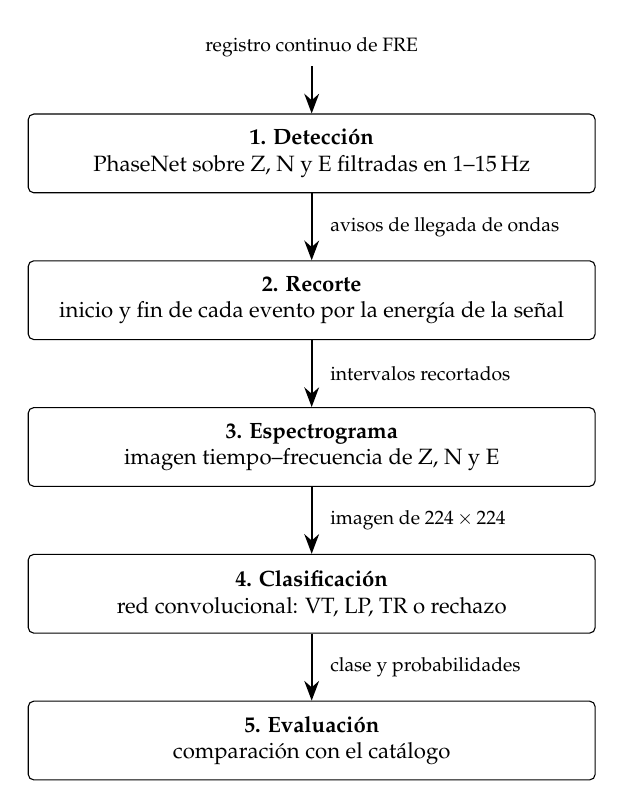
\begin{tikzpicture}[
  font=\footnotesize,
  etapa/.style={draw, rectangle, rounded corners=2pt, align=center,
    minimum height=1.0cm, minimum width=7.2cm, inner sep=4pt},
  flujo/.style={-{Stealth[length=2.5mm]}, thick},
  etiq/.style={font=\scriptsize, align=left}]
\node[etapa] (a) {\textbf{1. Detección}\\PhaseNet sobre Z, N y E filtradas en 1--15\,Hz};
\node[etapa, below=0.85cm of a] (b) {\textbf{2. Recorte}\\inicio y fin de cada evento por la energía de la señal};
\node[etapa, below=0.85cm of b] (c) {\textbf{3. Espectrograma}\\imagen tiempo--frecuencia de Z, N y E};
\node[etapa, below=0.85cm of c] (d) {\textbf{4. Clasificación}\\red convolucional: VT, LP, TR o rechazo};
\node[etapa, below=0.85cm of d] (e) {\textbf{5. Evaluación}\\comparación con el catálogo};
\node[above=0.6cm of a, etiq, align=center] (in) {registro continuo de FRE};
\draw[flujo] (in) -- (a);
\draw[flujo] (a) -- node[etiq, right=3pt] {avisos de llegada de ondas} (b);
\draw[flujo] (b) -- node[etiq, right=3pt] {intervalos recortados} (c);
\draw[flujo] (c) -- node[etiq, right=3pt] {imagen de 224\,$\times$\,224} (d);
\draw[flujo] (d) -- node[etiq, right=3pt] {clase y probabilidades} (e);
\end{tikzpicture}
\caption{Etapas de la cadena de procesamiento.}
\label{fig:arquitectura}
\end{figure}

\subsection{Datos que pasan de una etapa a otra}
\label{sec:contrato-datos}

Cada etapa deja un archivo que la siguiente lee, de modo que cualquier cifra
del informe se puede regenerar desde esos archivos. La detección deja los
avisos, con la fase (P o S), el instante y la probabilidad. El recorte deja
cada intervalo con su inicio y su fin en muestras de la señal. El etiquetado
deja, por recorte, la caja del catálogo que le corresponde, su IoU y su
etiqueta. El espectrograma deja los valores en decibelios de cada ventana. La
clasificación deja, por recorte, la clase elegida y la probabilidad de cada
clase, junto con un registro de la configuración usada, las versiones de las
librerías y las métricas de cada época de entrenamiento.

\section{Detección}
\label{sec:deteccion}

Un detector recorre la señal continua y avisa dónde parece haber un evento.
Se compararon tres (objetivo específico OE1, evaluar detectores): STA/LTA, un
método clásico que compara la energía reciente de la señal con la de un
periodo más largo \parencite{allen1978stalta}, y dos redes neuronales ya
entrenadas, PhaseNet \parencite{zhu2019phasenet} y EQTransformer
\parencite{mousavi2020eqtransformer}, usadas a través de la librería SeisBench
\parencite{woollam2022seisbench} con sus pesos ``original''. Ninguna de las
dos redes se reentrenó. La comparación y la elección se presentan en el
Capítulo~\ref{cap:resultados}; el sistema usa PhaseNet.

PhaseNet recibe Z, N y E y entrega, para cada instante, la probabilidad de que
en ese momento llegue una onda P (la primera onda de un sismo) y la de que
llegue una onda S (la segunda, más lenta). No entrega el fin del evento. Solo
se ajustan los parámetros que expone la propia librería: P\_threshold y
S\_threshold, la probabilidad mínima para considerar que llegó una onda P o S;
overlap, cuántas muestras se traslapan los tramos que la red analiza por
separado (1.500); blinding, cuántas muestras de cada borde de esos tramos se
descartan (250 por lado); y stacking, cómo se combinan los tramos traslapados
(promedio). La señal se filtra antes en 1--15\,Hz, porque PhaseNet no filtra
por su cuenta. La configuración usada es P\_threshold 0,40 y S\_threshold
0,05.

Cada vez que la probabilidad de P o de S supera su umbral se registra un
\emph{aviso} en el punto más alto de esa subida. Los avisos a 5\,s o menos
uno de otro se juntan en uno, porque suelen ser las ondas P y S de un mismo
evento.

La traza continua se entrega a PhaseNet en ventanas de 300\,s que avanzan de a
55\,s. Como el evento más largo del catálogo dura 240,8\,s, todo evento
queda completo dentro de al menos una ventana.

\section{Recorte por energía}
\label{sec:recorte}

PhaseNet dice dónde empieza un evento, pero no dónde termina. Para delimitarlo
se usa un recorte por energía, un método propio pedido por el profesor guía,
que sigue estos pasos:

\begin{enumerate}
\item Se calcula la \emph{envolvente} de la señal: en cada instante, la raíz
  de la energía promedio de Z, N y E durante el segundo que lo rodea.
\item Se mide el nivel del ruido antes del evento: el percentil 20 de la
  envolvente entre 120\,s y 5\,s antes del aviso. El percentil 20 se elige
  porque no lo altera la cola de un evento anterior. En las ventanas
  etiquetadas, ese periodo se toma solo dentro de la ventana.
\item El recorte empieza 2,5\,s antes del aviso, margen que cubre el error de
  inicio medido en la detección (entre 1,7 y 2,4\,s).
\item El recorte termina donde empieza el primer tramo de 5\,s en que la
  envolvente se mantiene bajo el doble del nivel del ruido, buscando entre 2 y
  300\,s después del aviso.
\item Si antes de ese fin llega otro aviso, el recorte se corta 2,5\,s antes
  de ese aviso, para no mezclar dos eventos.
\end{enumerate}

El recorte no usa ninguna información del catálogo: solo la señal y los
avisos de PhaseNet.

\section{Etiquetado de los recortes}
\label{sec:etiquetado}

Para entrenar y evaluar, cada recorte recibe una etiqueta según cuánto se
parece a una caja del catálogo. La medida es el IoU (\emph{intersection over
union}): el tiempo que el recorte y la caja tienen en común, dividido por el
tiempo total que cubren entre los dos. Vale 1 si coinciden exactamente y 0 si
no se tocan. Recortes y cajas se emparejan de a uno, empezando por los pares
de mayor IoU. Con ese emparejamiento:

\begin{itemize}
\item si el IoU es 0,3 o más, el recorte toma la clase de la caja; AV e IC
  pasan a la clase de rechazo;
\item si el recorte toca alguna caja pero con IoU menor, se marca ``fuera'' y
  no se usa, porque su delimitación es demasiado mala para asignarle una
  clase;
\item si no toca ninguna caja, se marca ``sin caja''. Puede ser una falsa
  alarma del detector o un evento que el catálogo no registra. No se usa para
  entrenar ni en las métricas del clasificador; solo se cuenta cuántos de ellos
  el clasificador llama volcánicos.
\end{itemize}

Sobre las 5.651 ventanas etiquetadas que tienen al menos un recorte, el
detector y el recorte producen 37.228 recortes, que se reparten como muestra
el Cuadro~\ref{tab:recortes-folds}.

{\small
\begin{longtable}{lrrrrrrrr}
\caption{Recortes de las ventanas etiquetadas por etiqueta y por parte del
conjunto.}\label{tab:recortes-folds}\\
\toprule
\textbf{Etiqueta} & \textbf{Fold 1} & \textbf{Fold 2} & \textbf{Fold 3} &
\textbf{Fold 4} & \textbf{Fold 5} & \textbf{Test} & \textbf{Total} \\
\midrule
\endfirsthead
\toprule
\textbf{Etiqueta} & \textbf{Fold 1} & \textbf{Fold 2} & \textbf{Fold 3} &
\textbf{Fold 4} & \textbf{Fold 5} & \textbf{Test} & \textbf{Total} \\
\midrule
\endhead
\bottomrule
\endlastfoot
VT & 245 & 235 & 240 & 262 & 256 & 336 & 1.574 \\
LP & 563 & 541 & 512 & 514 & 520 & 676 & 3.326 \\
TR & 210 & 203 & 221 & 200 & 188 & 244 & 1.266 \\
AV & 94 & 103 & 104 & 95 & 102 & 133 & 631 \\
IC & 123 & 151 & 142 & 127 & 145 & 191 & 879 \\
Fuera & 1.063 & 1.141 & 1.116 & 1.033 & 1.042 & 1.355 & 6.750 \\
Sin caja & 3.629 & 3.519 & 3.551 & 3.650 & 3.767 & 4.686 & 22.802 \\
\midrule
Total & 5.927 & 5.893 & 5.886 & 5.881 & 6.020 & 7.621 & 37.228 \\
\end{longtable}
}

\section{Espectrogramas}
\label{sec:recorte-espectrogramas}

El clasificador no recibe la señal, sino una imagen de ella: el
\emph{espectrograma}, que muestra cómo se reparte la energía de la señal entre
las frecuencias a lo largo del tiempo. El eje horizontal es el tiempo, el
vertical la frecuencia y el color la energía, en decibelios (dB), una escala
logarítmica.

Los espectrogramas se calculan sobre la ventana de 300\,s completa, con los
mismos parámetros con que se prepararon las ventanas etiquetadas: la señal se
filtra entre 1 y 15\,Hz con un filtro Butterworth de orden 15 aplicado hacia
adelante y hacia atrás, para no desplazarla en el tiempo; el espectrograma se
calcula en tramos de 256 muestras (2,56\,s) que avanzan de a 64, con ventana
de Hann y 512 puntos de frecuencia, y se conservan las frecuencias de 0 a
15\,Hz. Resultan 77 filas de frecuencia y 465 columnas de tiempo por ventana,
una columna cada 0,64\,s.

Los colores siguen la escala \emph{jet}, que va del azul oscuro al rojo. El
rojo corresponde a la energía máxima de cada componente en la ventana y el
azul más oscuro a 60\,dB bajo ese máximo; lo que queda más abajo se ve del
mismo azul. Z, N y E se apilan una sobre otra, de modo que cada imagen tiene
231 filas.

La imagen de un recorte son las columnas de la ventana que caen dentro de él.
Como los eventos duran distinto, las imágenes tienen anchos distintos, y las
redes necesitan una entrada de 224\,$\times$\,224 píxeles, el tamaño con que
fueron preentrenadas. Cada imagen se redimensiona a ese tamaño con
interpolación bilineal: se estira si tiene menos de 224 columnas y se comprime
si tiene más, sin cortar nada. No se usa el recorte central que traen las
redes por defecto, porque cortaría el inicio y el fin del evento. La
Figura~\ref{fig:estiramiento} muestra el proceso con un recorte corto y uno
largo.

\begin{figure}[!ht]
\centering
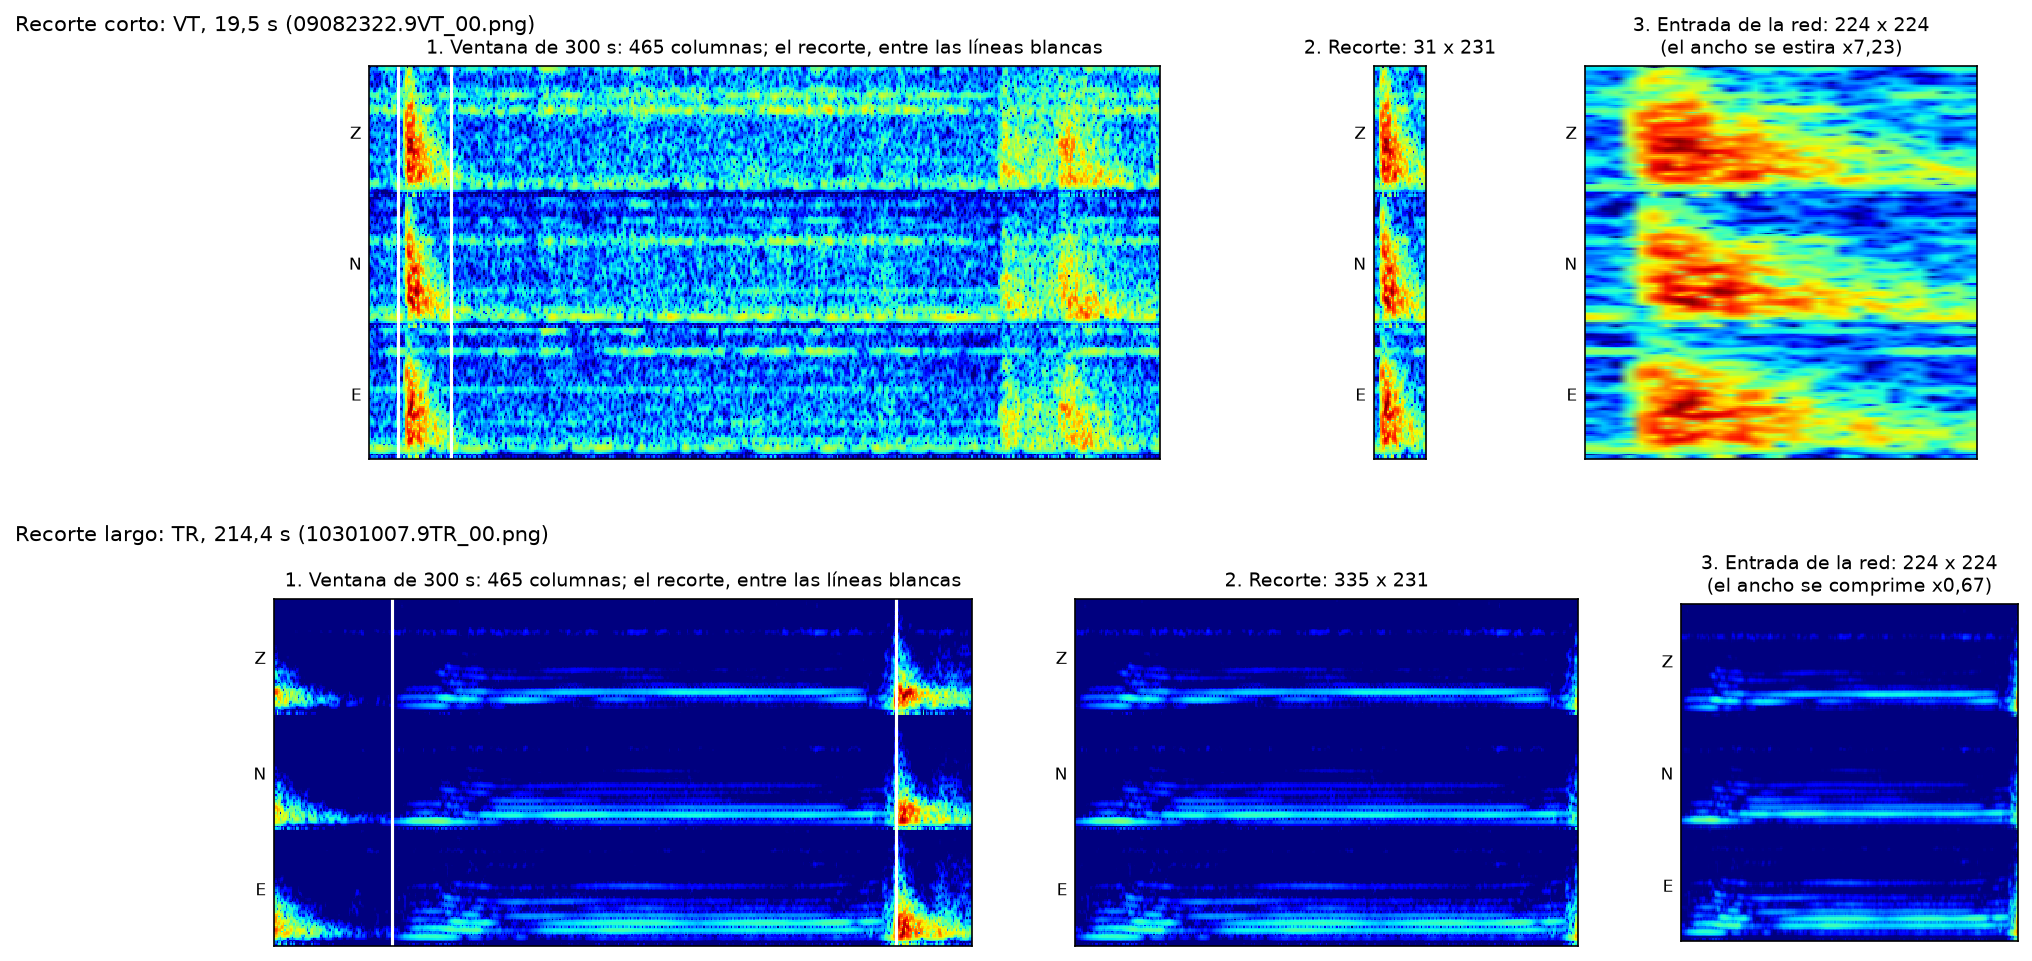
\includegraphics[width=\textwidth]{images/figura_estiramiento.png}
\caption{Del recorte a la entrada de la red. Arriba, un VT de 19,5\,s
(31 columnas), que se estira 7,23 veces; abajo, un TR de 214,4\,s
(335 columnas), que se comprime a 0,67. En cada fila: la ventana de 300\,s con
el recorte entre las líneas blancas, el recorte a su tamaño y la imagen de
224\,$\times$\,224 que recibe la red.}
\label{fig:estiramiento}
\end{figure}

Los recortes de menos de 5\,s se dejan fuera: al estirarlos, unas pocas
columnas se repiten decenas de veces y la imagen queda reducida a franjas
horizontales.

Como alternativa, el profesor guía pidió probar una duración fija: desde el
inicio de cada recorte se toman 60\,s de la ventana, sin importar cuánto dure
el evento. Si no alcanzan dentro de la ventana, se toman sus últimos 60\,s.
Estos resultados se muestran aparte, sin compararlos directamente con los del
recorte.

\section{Clasificador por transferencia de aprendizaje}
\label{sec:clasificador-transferencia}

\subsection{Redes}

Una red neuronal convolucional aprende a reconocer patrones en imágenes. En
vez de entrenarla desde cero, lo que requeriría muchas más imágenes, se parte
de una red ya entrenada con ImageNet, una colección de más de un millón de
fotografías de objetos comunes, y se ajusta a este problema \parencite{deng2009imagenet}. Esto se llama
\emph{transferencia de aprendizaje}: lo que la red aprendió a reconocer en
fotografías, como bordes, texturas y formas, sirve de punto de partida para
los espectrogramas.

Se comparan tres redes, todas de la librería torchvision con sus pesos
preentrenados por defecto: VGG16 \parencite{simonyan2015vgg}, que es la usada
por \textcite{espinosacurilem2025ood} en este mismo volcán; ResNet50
\parencite{he2016resnet}; y EfficientNet-B0 \parencite{tan2019efficientnet},
una red liviana. En las tres se reemplaza la última capa por una nueva con
cuatro salidas, una por clase: VT, LP, TR y rechazo. Se ajusta la red completa,
no solo la capa nueva. Las imágenes se normalizan con la media y la desviación
de ImageNet, igual que al preentrenar.

\subsection{Entrenamiento}

El entrenamiento muestra a la red las imágenes de cuatro folds y ajusta sus
pesos para que acierte la clase; el quinto fold se usa para validar, es decir,
para medir cómo le va con imágenes que no vio. Una pasada completa por las
imágenes de entrenamiento se llama \emph{época}. Los elementos que se ajustan
son los siguientes; todos son parámetros de PyTorch o torchvision
\parencite{paszke2019pytorch} y parten de su valor por defecto:

\begin{itemize}
\item Optimizador, el método que actualiza los pesos: AdamW
  \parencite{loshchilov2019adamw} o descenso de gradiente estocástico (SGD)
  con momentum 0,9.
\item Tasa de aprendizaje, el tamaño de cada ajuste de los pesos.
\item Weight decay, una penalización que evita pesos demasiado
  grandes.
\item Dropout, que durante el entrenamiento apaga al azar una
  fracción de las neuronas de las últimas capas para que la red no dependa de
  unas pocas \parencite{srivastava2014dropout}. VGG16 y EfficientNet-B0 lo
  traen como parámetro; a ResNet50, que no lo tiene, se le agrega una capa de
  dropout antes de la capa nueva.
\item Tamaño de lote, cuántas imágenes se usan en cada ajuste.
\item Función de pérdida, la medida del error que se minimiza. Se
  prueban dos: la entropía cruzada, con cada clase pesada por el inverso de su
  frecuencia para que las clases con menos ejemplos cuenten lo mismo, y la
  pérdida focal \parencite{lin2017focal}, que da más peso a los ejemplos
  difíciles, con sus valores por defecto en torchvision.
\end{itemize}

Las imágenes ``sin caja'' no se usan en el entrenamiento: la clase de rechazo
se forma solo con AV e IC.

Para decidir cuándo parar, después de cada época se mide en el fold de
validación el F1 macro de VT, LP y TR (definido en la
Sección~\ref{sec:protocolo}). Si no mejora durante 5 épocas seguidas, el
entrenamiento se detiene, con un máximo de 50 épocas. Se conservan los pesos de
la mejor época.

\subsection{Aumento de datos}
\label{subsec:aumento}

El aumento de datos modifica al azar las imágenes de entrenamiento en cada
época, para que la red vea variaciones de un mismo evento y no memorice las
imágenes exactas. Se aplica solo en el entrenamiento; la validación y el test
usan siempre las imágenes sin modificar. Se usan dos variaciones:

\begin{itemize}
\item Rango de colores. En vez de cambiar los colores de la imagen
  ya hecha, se cambia el rango en dB con que se colorea el espectrograma: el
  máximo se corre al azar entre $-5$ y $+5$\,dB y el ancho del rango se elige
  al azar entre 50 y 70\,dB, igual para las tres componentes. Así el mismo
  evento aparece con sus componentes más o menos marcadas, como un evento con
  más o menos ruido. La Figura~\ref{fig:rangos} muestra el efecto con límites
  más amplios que los usados.
\item Deformación elástica, que desplaza suavemente los píxeles de
  la imagen \parencite{simard2003elastic}, con la función ElasticTransform de
  torchvision y sus valores por defecto (alpha 50 y sigma 5). Se aplica solo
  en el eje del tiempo, porque deformar la frecuencia cambiaría justamente lo
  que distingue a un LP de un VT. La Figura~\ref{fig:elastica} compara las dos
  opciones.
\end{itemize}

No se usa el recorte aleatorio de la imagen, porque podría quitar el inicio o
el fin del evento. Los límites del rango de colores y la elección del eje de la
deformación son decisiones propias de este trabajo.

\begin{figure}[!ht]
\centering
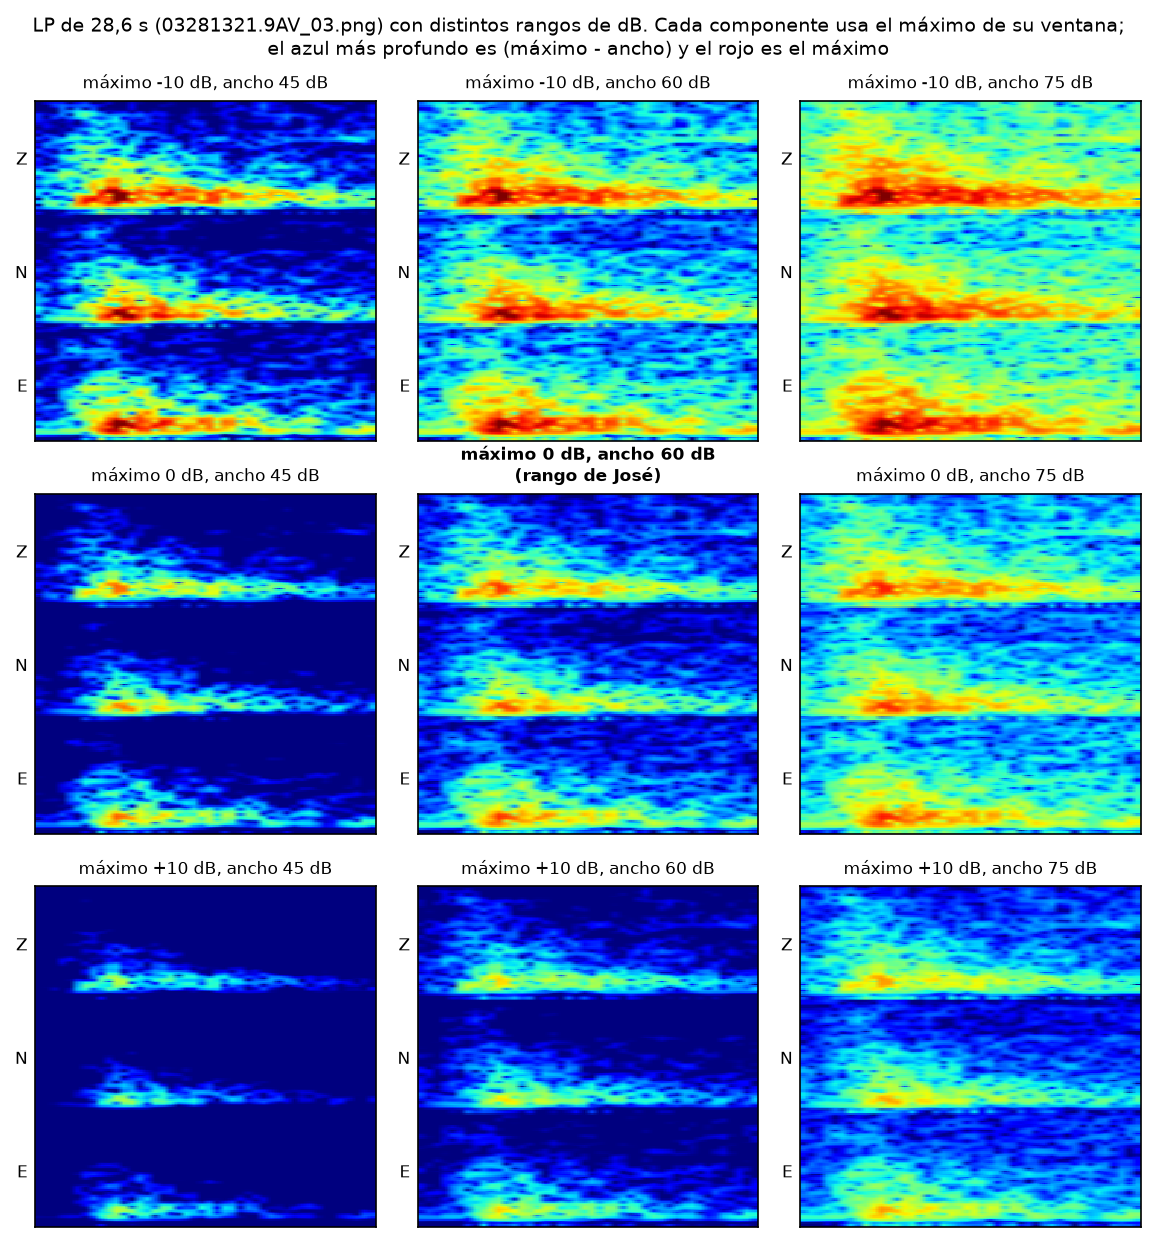
\includegraphics[width=0.85\textwidth]{images/figura_rangos_db.png}
\caption{Un mismo LP coloreado con distintos rangos de dB. Al centro, el rango
de las imágenes sin aumento: el máximo de cada componente y 60\,dB bajo él.
En el entrenamiento se usan corrimientos de hasta 5\,dB y anchos entre 50 y
70\,dB.}
\label{fig:rangos}
\end{figure}

\begin{figure}[!ht]
\centering
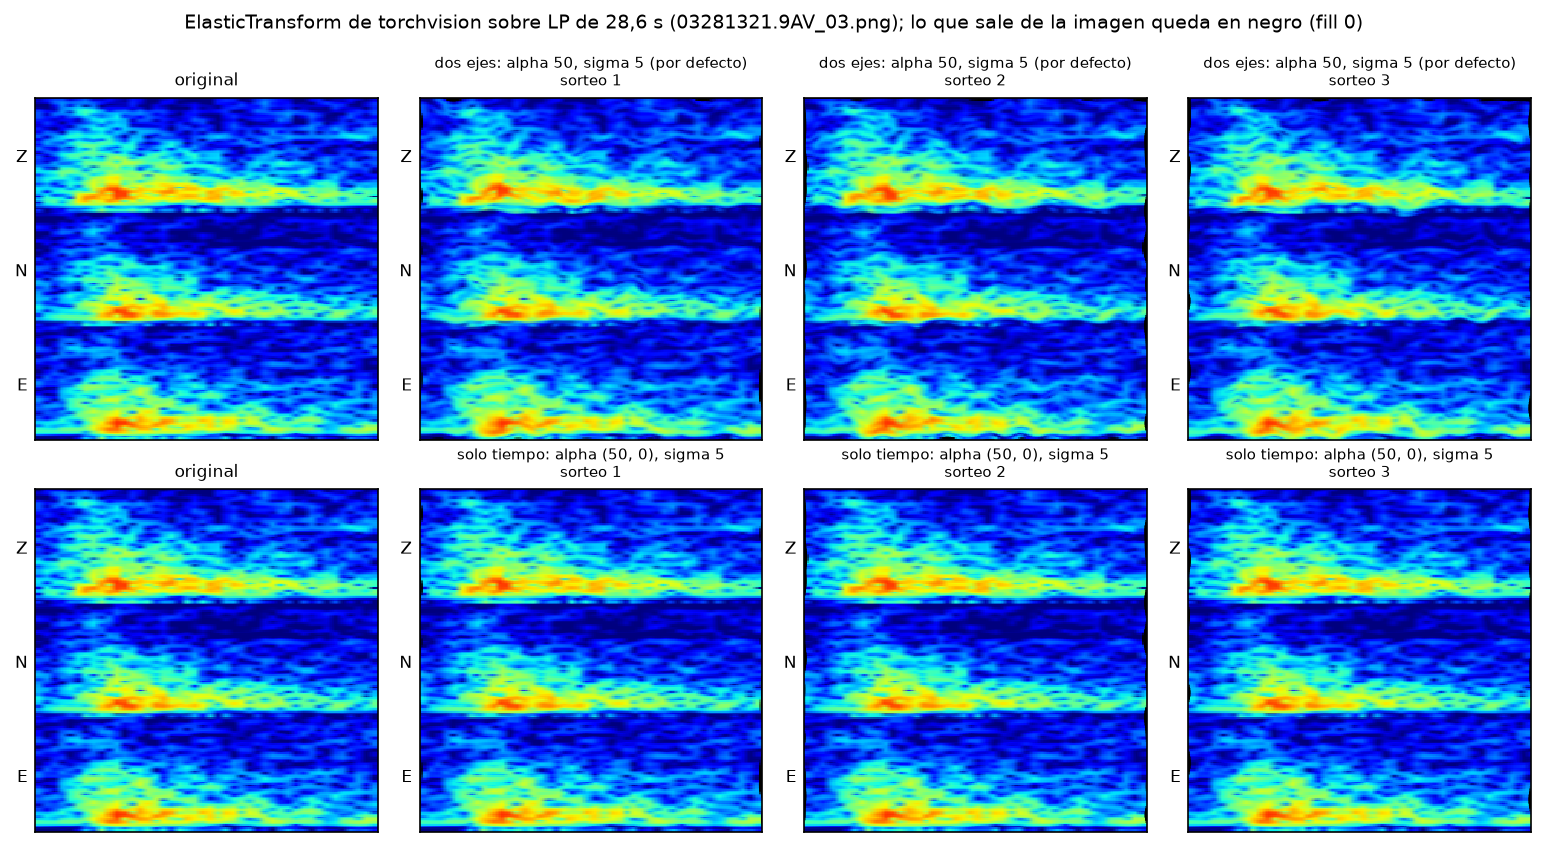
\includegraphics[width=\textwidth]{images/figura_elastica.png}
\caption{Deformación elástica sobre el mismo LP. Arriba, en los dos ejes: las
líneas de frecuencia se ondulan. Abajo, solo en el eje del tiempo, que es la
opción usada: las frecuencias quedan en su lugar.}
\label{fig:elastica}
\end{figure}

\subsection{Búsqueda de la configuración}
\label{subsec:busqueda}

Para elegir la combinación de parámetros de cada red se hace una búsqueda
bayesiana con Optuna \parencite{akiba2019optuna}, con su método por defecto,
TPE \parencite{bergstra2011tpe}. En vez de probar todas las combinaciones, que
serían 128 por red, este método mira cómo resultaron las pruebas anteriores y
propone las siguientes en las zonas que funcionaron mejor. Se hacen 20 pruebas
por red, entrenando con los folds 2 a 5 y validando con el fold 1, y se elige
la combinación con mayor F1 macro de VT, LP y TR en validación. El
Cuadro~\ref{tab:espacio} muestra los valores probados.

{\small
\begin{longtable}{>{\raggedright\arraybackslash}p{4.2cm}>{\raggedright\arraybackslash}p{7.2cm}}
\caption{Valores probados en la búsqueda de la configuración.}\label{tab:espacio}\\
\toprule
\textbf{Parámetro} & \textbf{Valores} \\
\midrule
\endfirsthead
\toprule
\textbf{Parámetro} & \textbf{Valores} \\
\midrule
\endhead
\bottomrule
\endlastfoot
Optimizador & AdamW; SGD con momentum 0,9 \\
Tasa de aprendizaje & 0,01; 0,001; 0,0001; 0,00001 \\
Dropout & 0,2; 0,3 \\
Tamaño de lote & 16; 32 \\
Weight decay & 0; 0,0001 \\
Función de pérdida & entropía cruzada con pesos por clase; pérdida focal \\
\midrule
Fijos & ajuste de la red completa; duración mínima de 5\,s; sin las imágenes
``sin caja''; máximo 50 épocas; parada temprana con paciencia 5; aumento de
datos de la Sección~\ref{subsec:aumento} \\
\end{longtable}
}

\subsection{Validación cruzada y test}

Con la combinación elegida, cada red se entrena cinco veces: en cada una se
valida con un fold distinto y se entrena con los otros cuatro. El mejor modelo
de cada una de esas cinco corridas se evalúa sobre las ventanas de test, que
no participaron en ninguna decisión. Así se obtienen cinco valores de cada
métrica, de los que se informan el promedio, el mínimo, el máximo y la
desviación estándar. Todo se repite con la ventana fija de 60\,s.

El entrenamiento se hizo en un servidor con una GPU NVIDIA RTX 5090 de la
universidad, con PyTorch 2.14 y CUDA 13.0, enviando cada corrida a la cola de
trabajos del servidor (Slurm). La semilla de los generadores de números al azar se fija para que
cada corrida se pueda repetir.

\section{Protocolo de evaluación}
\label{sec:protocolo}

\subsection{Métricas}

Para cada clase se cuentan los aciertos y los errores del sistema contra el
catálogo:

\begin{itemize}
\item Sensibilidad: de los eventos de una clase, la fracción que el
  sistema encuentra o clasifica bien. Es la métrica de la meta del trabajo,
  que es llegar a 0,95.
\item Precisión: de lo que el sistema asigna a una clase, la
  fracción que de verdad es de esa clase.
\item F1: combina las dos anteriores en un solo número (su media
  armónica); es alto solo si ambas lo son.
\item F1 macro de VT, LP y TR: el promedio simple del F1 de las tres
  clases volcánicas, de modo que cada clase pesa lo mismo aunque tenga menos
  ejemplos.
\item Matriz de confusión normalizada por fila: para cada clase real,
  qué fracción de sus eventos se asignó a cada clase. La diagonal es la
  sensibilidad de cada clase y el resto muestra con qué se confunde.
\end{itemize}

No se usa la exactitud global (el porcentaje total de aciertos), porque las
clases tienen tamaños muy distintos: LP reúne cerca de la mitad de los
eventos, y una red podría acertar mucho LP y fallar TR con una exactitud alta.

\subsection{Detección y recorte}

En la comparación de detectores sobre la traza continua, un evento cuenta como
detectado si hay un aviso a 5\,s o menos de su inicio, antes o después, y cada
aviso cuenta para un solo evento; la misma regla se aplica a los tres
detectores. En las ventanas de test, un evento cuenta como detectado si alguno
de los intervalos en que la probabilidad de P o de S de PhaseNet supera su
umbral se cruza con su caja. La calidad del recorte se mide con el IoU contra
la caja, informando qué fracción de los eventos tiene un recorte con IoU de
0,3 o más y de 0,5 o más. Las falsas alarmas se informan como recortes sin
caja por hora de registro, y su proporción entre todos los recortes como FDR
(\emph{false discovery rate}).

\subsection{Sistema completo sobre la traza continua}

El objetivo específico OE4 pide evaluar el sistema integrado sobre registros
continuos. Para eso la cadena completa se aplica a la traza de FRE:

\begin{enumerate}
\item PhaseNet en ventanas de 300\,s que avanzan de a 55\,s, y el recorte por
  energía de la Sección~\ref{sec:recorte}.
\item Para cada recorte, una ventana de 300\,s centrada en él, como las
  ventanas etiquetadas, que tienen su evento principal al centro; sin salir de
  su tramo. Su espectrograma se calcula sobre la señal de FRE sin filtrar,
  para aplicar el mismo filtro y los mismos parámetros que en el entrenamiento,
  y el rango de dB se toma del máximo de esa ventana.
\item Cada recorte se clasifica con los cinco modelos de cada red (uno por
  fold), y se informan el promedio, el mínimo, el máximo y la desviación entre
  los cinco.
\item Los recortes se etiquetan contra el catálogo con la misma regla de la
  Sección~\ref{sec:etiquetado}.
\end{enumerate}

Se informan tres medidas. La primera es la clasificación de los recortes que
calzan con un evento del catálogo (IoU de 0,3 o más). La segunda es la
\emph{sensibilidad completa} de cada clase: la fracción de sus eventos que el
sistema detecta, recorta con IoU de 0,3 o más y clasifica en la clase
correcta, todo a la vez. La tercera son las falsas alarmas por hora que el
clasificador llama volcánicas. Además se mide el tiempo de cada etapa.

Como la traza tiene pocos eventos por clase (entre 24 y 50 recortes que calzan
con un evento), cada sensibilidad se acompaña de su intervalo de confianza de
95\,\% según el método de \textcite{wilson1927}, para distinguir las
diferencias reales de las que se deben al tamaño de la muestra.

\chapter{Resultados}
\label{cap:resultados}

Este capítulo presenta lo que se midió en cada etapa de la cadena descrita en
el Capítulo~\ref{cap:diseno}, en el mismo orden en que la recorre la señal.
Primero se comparan los tres detectores sobre la traza continua y se mide la
calidad de sus recortes (objetivos OE1 y OE2: evaluar los detectores y
delimitar los eventos). Luego se mide la detección en las ventanas de test, se
presentan la búsqueda de la configuración y la validación cruzada del
clasificador (OE3: ajustar la red por transferencia de aprendizaje) y, por
último, el sistema completo aplicado a la traza continua (OE4: evaluar el
sistema integrado). El capítulo termina con las comprobaciones que se hicieron
para entender por qué el clasificador acierta menos en la traza que en test.
Todas las cifras se midieron sobre datos reales; su interpretación se discute
en el Capítulo~\ref{cap:discusion}.

% =====================================================================
\section{Comparación de detectores}
\label{sec:res-detectores}

Los tres detectores se evaluaron sobre la traza continua de FRE con los 125
eventos volcánicos del catálogo que tienen registro de las tres componentes:
36 VT, 52 LP y 37 TR. Los 6 AV y 48 IC que también tienen registro se informan
aparte. Todos se cuentan con la intersección descrita en la
Sección~\ref{subsec:protocolo-deteccion}: un evento está detectado si algún
intervalo del detector comparte al menos un instante con él, y una falsa
alarma es un intervalo que no toca ningún evento del catálogo. Las falsas
alarmas se cuentan por hora de registro (FP/h).

\subsection{Parámetros probados}
\label{subsec:res-parametros}

El Cuadro~\ref{tab:res-parametros} reúne los parámetros de cada detector, su
valor por defecto y los valores que se probaron. Solo se movieron parámetros
que expone la librería de cada detector, con el nombre que esta les da y
partiendo de su valor por defecto. Cada umbral se probó con 21 valores: 0,02,
0,03, 0,05 y de 0,10 a 0,95 cada 0,05. Los pasos son más finos bajo 0,10
porque ahí están los valores con que las redes detectan más.

{\small
\setlength{\tabcolsep}{4pt}
\begin{longtable}{>{\raggedright\arraybackslash}p{2.9cm}>{\raggedright\arraybackslash}p{4.5cm}>{\raggedright\arraybackslash}p{1.8cm}>{\raggedright\arraybackslash}p{3.0cm}}
\caption{Parámetros de cada detector. ``Por defecto'' es el valor que trae la
librería; en SeisBench, el que carga con los pesos ``original''.}\label{tab:res-parametros}\\
\cabecera{\textbf{Parámetro} & \textbf{Qué hace} & \textbf{Por defecto} & \textbf{Valores probados}}{4}
\multicolumn{4}{l}{\textit{PhaseNet (SeisBench)}}\\*
\texttt{P\_threshold} & Probabilidad mínima para aceptar una onda P & 0,3 & 0,02 a 0,95 \\
\texttt{S\_threshold} & Lo mismo para la onda S & 0,3 & 0,02 a 0,95, por separado del de P \\
\texttt{overlap} & Muestras que comparten dos ventanas seguidas de la red & 1500 (15\,s) & 500 a 2500 \\
\texttt{blinding} & Muestras que se descartan en cada borde de la ventana, donde la red ve señal hacia un solo lado & 250 por lado & 0 a 500 \\
\texttt{stacking} & Cómo se juntan las predicciones de ventanas que se solapan: promedio (\texttt{avg}) o máximo (\texttt{max}) & \texttt{avg} & \texttt{avg} y \texttt{max} \\
\midrule
\multicolumn{4}{l}{\textit{EQTransformer (SeisBench)}}\\*
\texttt{detection\_\allowbreak threshold} & Probabilidad mínima de la curva de detección & 0,3 & 0,02 a 0,95 \\
\texttt{P\_threshold}, \texttt{S\_threshold} & Probabilidad mínima de la onda P y de la onda S & 0,1 & 0,02 a 0,95, cada uno por separado \\
\texttt{overlap} & Igual que en PhaseNet & 3000 (30\,s) & 1000 a 5000 \\
\texttt{blinding} & Igual que en PhaseNet & 500 por lado & 0 a 1000 \\
\texttt{stacking} & Igual que en PhaseNet & \texttt{max} & \texttt{avg} y \texttt{max} \\
Filtro interno & Deja pasar 1--45\,Hz antes de entrar a la red & 1--45\,Hz & No se puede cambiar; viene con los pesos \\
\midrule
\multicolumn{4}{l}{\textit{STA/LTA (ObsPy)}}\\*
\texttt{nsta}, \texttt{nlta} & Largo de la ventana corta y de la larga & No tiene & 2 y 60\,s, sin cambio \\
\texttt{thres1}, \texttt{thres2} & Razón STA/LTA que enciende y que apaga el aviso & No tiene & 4,0 y 1,05, sin cambio \\
\texttt{freqmin}, \texttt{freqmax} & Banda del filtro previo & No tiene & 1 y 20\,Hz, sin cambio \\
\end{longtable}
}

Las redes no leen la traza de una vez, sino por ventanas: de 30\,s en PhaseNet
y de 60\,s en EQTransformer. Los parámetros \texttt{overlap},
\texttt{blinding} y \texttt{stacking} deciden cómo se recorren y se juntan esas
ventanas. A diferencia de los umbrales, cambian las curvas de probabilidad, así
que con cada combinación se volvió a correr la red sobre toda la traza. Se
omitieron las combinaciones con \texttt{overlap} menor que el doble de
\texttt{blinding}, porque descartan más de lo que se solapan y dejan tramos sin
predicción. Quedan 38 combinaciones por red; junto con los umbrales suman
16.758 casos en PhaseNet y 17.556 en EQTransformer. STA/LTA mantiene la
configuración que se eligió con un barrido en una evaluación anterior de este
trabajo, y usa solo la componente vertical.

Las dos redes reciben Z, N y E filtradas en 1--15\,Hz, la banda de la traza
publicada. También se probó la banda de 1--45\,Hz, la del filtro interno de
EQTransformer. Con ella PhaseNet necesita 73,9 falsas alarmas por hora para
llegar a 0,95, en vez de 69,0; EQTransformer llega al mismo máximo con su curva
de detección (0,864) y a uno menor con P y S (0,728 en vez de 0,736), y STA/LTA
detecta 105 volcánicos en vez de 106. Como no mejora a ningún detector, todo lo
que sigue usa 1--15\,Hz.

\subsection{Resultado con un umbral común}

Como punto de partida, el Cuadro~\ref{tab:res-umbral010} muestra los
detectores con el mismo umbral, 0,10, y las ventanas por defecto de las redes.
EQTransformer aparece dos veces porque entrega dos salidas: su curva de
detección y sus curvas de P y S. Las dos últimas columnas dan los volcánicos
que se contaban con el criterio anterior, con un aviso a 5 o a 10\,s del
inicio del evento.

{\small
\setlength{\tabcolsep}{3pt}
\begin{longtable}{>{\raggedright\arraybackslash}p{3.4cm}rrrrrrr}
\caption{Detección con umbral 0,10 en las redes. Volcánicos: detectados de 125.
Las dos últimas columnas usan el criterio anterior.}\label{tab:res-umbral010}\\
\cabecera{ & \multicolumn{5}{c}{\textbf{Intersección}} & \multicolumn{2}{c}{\textbf{Aviso a}} \\ \textbf{Detector} & \textbf{VT} & \textbf{LP} & \textbf{TR} & \textbf{Volcánicos} & \textbf{FP/h} & \textbf{5\,s} & \textbf{10\,s}}{8}
PhaseNet, P y S & 34/36 & 49/52 & 34/37 & 117 = 0,936 & 62,7 & 113 & 121 \\
EQTransformer, detección & 27/36 & 43/52 & 22/37 & 92 = 0,736 & 7,9 & 69 & 72 \\
EQTransformer, P y S & 22/36 & 33/52 & 16/37 & 71 = 0,568 & 9,3 & 67 & 70 \\
STA/LTA & 32/36 & 44/52 & 30/37 & 106 = 0,848 & 19,0 & 89 & 99 \\
\end{longtable}
}

Con la intersección, PhaseNet detecta 117 de los 125 volcánicos (0,936). Con el
criterio anterior la cifra dependía de la tolerancia: 113 con 5\,s y 121 con
10\,s. Los 8 eventos de diferencia entre 5 y 10\,s son todos TR: 6 tienen
su aviso entre 5 y 10\,s después del inicio y 2, entre 5 y 10\,s antes. Frente
al criterio de 5\,s, la intersección le suma a PhaseNet 8 TR cuyo intervalo
cae dentro del evento (en 6, entre 4,6 y 8,2\,s después del inicio; en 2, a
los 22 y 42\,s) y le resta 4 eventos (3 LP y 1 VT) cuyo intervalo termina
entre 0,0 y 1,1\,s antes del inicio que marca el catálogo. Con estos datos no
se puede saber si en esos cuatro el catálogo marca el inicio algo tarde o si
PhaseNet avisa antes de tiempo. EQTransformer con su curva de detección sube
de 69 a 92 y STA/LTA de 89 a 106, porque muchos de sus intervalos empiezan
bastante antes del evento y siguen dentro de él, o caen dentro del evento más
de 5\,s después de su inicio. Que un intervalo toque el evento no dice si sirve
para recortarlo; eso se mide con el IoU en la Sección~\ref{sec:res-recorte}.

\subsection{Barrido de umbrales y de ventanas}

El Cuadro~\ref{tab:res-metas} muestra con qué umbrales llega cada detector a
tres metas de sensibilidad volcánica, con las ventanas por defecto. Cuando
varias combinaciones llegan a la meta, se muestra la de menos falsas alarmas.

{\small
\setlength{\tabcolsep}{3pt}
\begin{longtable}{>{\raggedright\arraybackslash}p{2.7cm}>{\raggedright\arraybackslash}p{2.3cm}>{\raggedright\arraybackslash}p{2.3cm}>{\raggedright\arraybackslash}p{2.3cm}>{\raggedright\arraybackslash}p{2.6cm}}
\caption{Umbrales con que cada detector llega a cada meta de sensibilidad
volcánica, con las ventanas por defecto. Entre paréntesis, volcánicos
detectados y FP/h.}\label{tab:res-metas}\\
\cabecera{\textbf{Detector} & \textbf{Meta 0,80} & \textbf{Meta 0,90} & \textbf{Meta 0,95} & \textbf{Máximo}}{5}
PhaseNet, P y S & P 0,40 y S 0,25 (101; 28,6) & P 0,40 y S 0,15 (114; 41,8) & P 0,40 y S 0,05 (119; 69,0) & 0,984 con P 0,03 y S 0,02 (123; 104,4) \\
EQTransformer, detección & umbral 0,05 (100; 10,3) & No llega & No llega & 0,864 con umbral 0,02 (108; 13,1) \\
EQTransformer, P y S & No llega & No llega & No llega & 0,736 con P 0,03 y S 0,02 (92; 14,4) \\
STA/LTA (sin barrido) & Llega (106; 19,0) & No llega & No llega & 0,848 (106; 19,0) \\
\end{longtable}
}

Con las ventanas por defecto, solo PhaseNet llega a 0,95. Lo hace con
\texttt{P\_threshold} en 0,40 en las tres metas; lo que cambia de una a otra es
\texttt{S\_threshold}, que baja de 0,25 a 0,15 y a 0,05. Bajar el umbral de la
onda S suma volcánicos, sobre todo LP y TR, en que la onda P no da aviso.

Al cambiar también las ventanas, EQTransformer mejora mucho. Con
\texttt{overlap} en 4000, \texttt{blinding} en 0 y \texttt{stacking} en
\texttt{max}, su curva de detección sube de 0,864 a 0,936, con 52,7 falsas
alarmas por hora, y con P y S sube de 0,736 a 0,872 (\texttt{overlap} 5000,
\texttt{blinding} 500, \texttt{max}), con 25,0. Aun así, ninguna combinación de
EQTransformer llega a 0,95. En PhaseNet la sensibilidad casi no cambia, porque
ya llega a 0,95 con las ventanas por defecto; lo que cambia son las falsas
alarmas que cuesta llegar, que bajan de 69,0 a 48,1 por hora con
\texttt{overlap} 2500, \texttt{blinding} 0, \texttt{max} y umbrales de 0,95
para P y 0,25 para S.

\subsection{Rotación de tramos}

Todos los valores anteriores se eligieron mirando la misma traza con que se
evalúan. Para medir cuánto pesa eso se hizo la rotación de tramos descrita en
la Sección~\ref{subsec:protocolo-deteccion}: elegir con dos tramos y medir en
el tercero. Los volcánicos no están repartidos parejo entre los tramos
(Cuadro~\ref{tab:res-tramos}). El tramo 1 tiene casi todos los LP y TR, el 2
tiene sobre todo VT y el 3 casi solo IC, así que en la práctica la prueba
compara los tramos 1 y 2, que tienen eventos de distinto tipo.

{\small
\setlength{\tabcolsep}{5pt}
\begin{longtable}{lrrrrrrr}
\caption{Eventos evaluados por tramo y horas con registro.}\label{tab:res-tramos}\\
\cabecera{\textbf{Tramo} & \textbf{Horas} & \textbf{VT} & \textbf{LP} & \textbf{TR} & \textbf{Volcánicos} & \textbf{AV} & \textbf{IC}}{8}
1 & 5,75 & 12 & 48 & 33 & 93 & 2 & 12 \\
2 & 2,82 & 22 & 4 & 4 & 30 & 2 & 9 \\
3 & 1,16 & 2 & 0 & 0 & 2 & 2 & 27 \\
\midrule
Total & 9,73 & 36 & 52 & 37 & 125 & 6 & 48 \\
\end{longtable}
}

El Cuadro~\ref{tab:res-rotacion} compara, para cada red, la elección con la
traza completa y con la rotación. En cada caso se prueban las dos opciones de
la regla de elección: mover solo los umbrales o mover umbrales y ventanas.

{\small
\setlength{\tabcolsep}{4pt}
\begin{longtable}{>{\raggedright\arraybackslash}p{5.4cm}>{\raggedright\arraybackslash}p{3.4cm}>{\raggedright\arraybackslash}p{3.4cm}}
\caption{Elección con la traza completa y con la rotación de tramos.
Volcánicos detectados de 125 y FP/h.}\label{tab:res-rotacion}\\
\cabecera{\textbf{Detector y qué se elige} & \textbf{Traza completa} & \textbf{Rotación de tramos}}{3}
PhaseNet, solo umbrales & 119 = 0,952; 69,0 & 120 = 0,960; 79,7 \\
PhaseNet, umbrales y ventanas & 120 = 0,960; 48,1 & 116 = 0,928; 59,5 \\
\midrule
EQTransformer detección, solo umbral & 108 = 0,864; 13,1 & 108 = 0,864; 13,1 \\
EQTransformer detección, umbral y ventanas & 117 = 0,936; 52,7 & 114 = 0,912; 42,3 \\
\midrule
EQTransformer P y S, solo umbrales & 92 = 0,736; 14,4 & 89 = 0,712; 12,2 \\
EQTransformer P y S, umbrales y ventanas & 109 = 0,872; 25,0 & 103 = 0,824; 18,4 \\
\end{longtable}
}

Con solo los umbrales, PhaseNet mantiene la meta al medir en tramos que no se
usaron para elegir: 120 de 125 (0,960). Con las ventanas, la mejora en falsas
alarmas no se sostiene y la sensibilidad baja a 116 (0,928), bajo la meta: con
más parámetros para elegir, la elección se ajusta más a los tramos con que se
hace. En EQTransformer, en cambio, las ventanas mejoran también en la
rotación: su curva de detección pasa de 0,864 a 0,912.

\subsection{Configuración elegida}
\label{subsec:res-configuracion}

El Cuadro~\ref{tab:res-config} muestra lo que resulta de aplicar la regla de
elección a cada red. En PhaseNet la regla deja las ventanas por defecto,
porque cambiarlas no se sostiene en la rotación; en EQTransformer las cambia,
porque ahí sí se sostiene.

{\small
\setlength{\tabcolsep}{3pt}
\begin{longtable}{>{\raggedright\arraybackslash}p{2.7cm}>{\raggedright\arraybackslash}p{2.6cm}>{\raggedright\arraybackslash}p{3.6cm}rr}
\caption{Configuración de cada detector. Entre paréntesis, la sensibilidad en
la rotación de tramos de la opción elegida y de la otra.}\label{tab:res-config}\\
\cabecera{\textbf{Detector} & \textbf{Opción} & \textbf{Valores} & \textbf{Volcánicos} & \textbf{FP/h}}{5}
PhaseNet, P y S & Solo umbrales (0,960 contra 0,928) & P 0,40 y S 0,05; \texttt{overlap} 1500, \texttt{blinding} 250, \texttt{avg} & 119 = 0,952 & 69,0 \\
EQTransformer, detección & Umbral y ventanas (0,912 contra 0,864) & umbral 0,02; \texttt{overlap} 4000, \texttt{blinding} 0, \texttt{max} & 117 = 0,936 & 52,7 \\
EQTransformer, P y S & Umbrales y ventanas (0,824 contra 0,712) & P 0,03 y S 0,02; \texttt{overlap} 5000, \texttt{blinding} 500, \texttt{max} & 109 = 0,872 & 25,0 \\
STA/LTA & Sin barrido & ventanas de 2 y 60\,s; razones 4,0 y 1,05; 1--20\,Hz & 106 = 0,848 & 19,0 \\
\end{longtable}
}

Solo PhaseNet llega a la meta de 0,95. EQTransformer, con su curva de
detección, queda cerca (0,936) y con menos falsas alarmas, pero no llega. El
Cuadro~\ref{tab:res-clase} separa por clase lo que detecta cada uno. Entre
corchetes va el intervalo de confianza del 95\,\% de \textcite{wilson1927}: el
rango en que probablemente estaría la sensibilidad con otro grupo de eventos
parecido. La FDR (\emph{false discovery rate}) es la parte de las detecciones
que son falsas alarmas: las falsas alarmas divididas por la suma de
volcánicos detectados y falsas alarmas.

{\footnotesize
\setlength{\tabcolsep}{3pt}
\begin{longtable}{>{\raggedright\arraybackslash}p{1.9cm}>{\raggedright\arraybackslash}p{2.6cm}>{\raggedright\arraybackslash}p{2.6cm}>{\raggedright\arraybackslash}p{2.6cm}>{\raggedright\arraybackslash}p{2.6cm}}
\caption{Detección por clase con la configuración de cada detector.}\label{tab:res-clase}\\
\cabecera{\textbf{Clase} & \textbf{PhaseNet, P y S} & \textbf{EQTransformer, detección} & \textbf{EQTransformer, P y S} & \textbf{STA/LTA}}{5}
VT & 34/36 [0,819; 0,985] & 30/36 [0,681; 0,921] & 30/36 [0,681; 0,921] & 32/36 [0,747; 0,956] \\
LP & 50/52 [0,870; 0,989] & 52/52 [0,931; 1,000] & 47/52 [0,794; 0,958] & 44/52 [0,725; 0,920] \\
TR & 35/37 [0,823; 0,985] & 35/37 [0,823; 0,985] & 32/37 [0,720; 0,941] & 30/37 [0,658; 0,905] \\
\midrule
\textbf{Volcánicos} & 119/125 = 0,952 [0,899; 0,978] & 117/125 = 0,936 [0,879; 0,967] & 109/125 = 0,872 [0,802; 0,920] & 106/125 = 0,848 [0,775; 0,900] \\
\midrule
AV (rechazo) & 6/6 & 3/6 & 3/6 & 4/6 \\
IC (rechazo) & 35/48 & 32/48 & 20/48 & 25/48 \\
\midrule
FP/h & 69,0 & 52,7 & 25,0 & 19,0 \\
FDR & 0,85 & 0,81 & 0,69 & 0,64 \\
\end{longtable}
}

PhaseNet pierde 2 VT, 2 LP y 2 TR. EQTransformer con su curva de detección
encuentra todos los LP, pero pierde 6 VT. Con PhaseNet la FDR es 0,85, es
decir, hay unas 5,7 falsas alarmas por cada volcánico detectado. El intervalo
de confianza de su sensibilidad va de 0,899 a 0,978: con 125 eventos, el valor
medido pasa la meta, pero el intervalo incluye valores bajo ella.

La Figura~\ref{fig:res-curvas} muestra cómo cambian la sensibilidad de cada
clase y la FDR al mover un umbral, con las ventanas de la configuración de
cada red. En los paneles de P y S se mueve uno de los dos umbrales y el otro
queda en el valor elegido. La línea punteada vertical marca el valor elegido y
la horizontal, la meta de 0,95.

\begin{figure}[!ht]
\centering
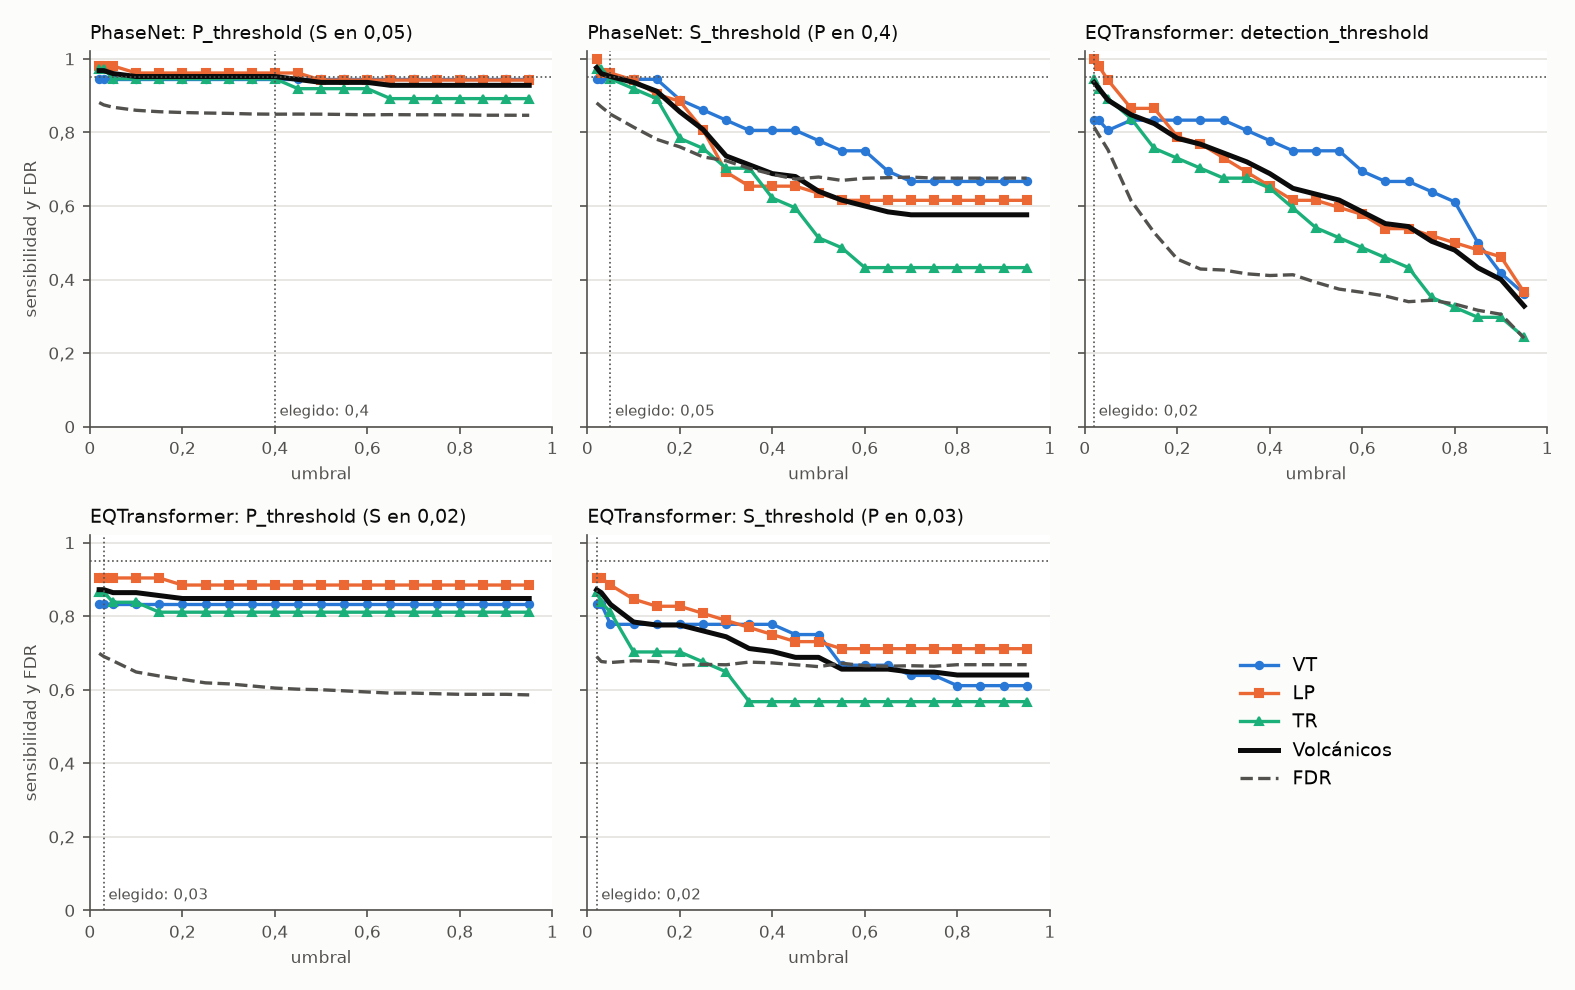
\includegraphics[width=\textwidth]{figuras/fig8_curvas_interseccion.png}
\caption{Sensibilidad por clase, sensibilidad volcánica y FDR según el umbral,
con la intersección y las ventanas de la configuración de cada red.}
\label{fig:res-curvas}
\end{figure}

En PhaseNet, con \texttt{S\_threshold} en 0,05, mover \texttt{P\_threshold}
casi no cambia la sensibilidad, porque la onda S detecta la mayor parte de los
volcánicos. Con \texttt{P\_threshold} en 0,40, en cambio, subir
\texttt{S\_threshold} baja la sensibilidad en todas las clases, y más en TR,
que cae a 0,43 cuando el umbral pasa de 0,60. En EQTransformer ocurre lo mismo
con sus umbrales de P y S. Con su curva de detección, la sensibilidad y la FDR
bajan juntas al subir el umbral.

La Figura~\ref{fig:res-costo} muestra el costo de cada nivel de sensibilidad
en falsas alarmas por hora. Cada punto es una combinación de umbrales con las
ventanas de la configuración de cada red; los puntos grandes son las
configuraciones elegidas, y STA/LTA aparece como un solo punto porque sus
parámetros no se mueven.

\begin{figure}[!ht]
\centering
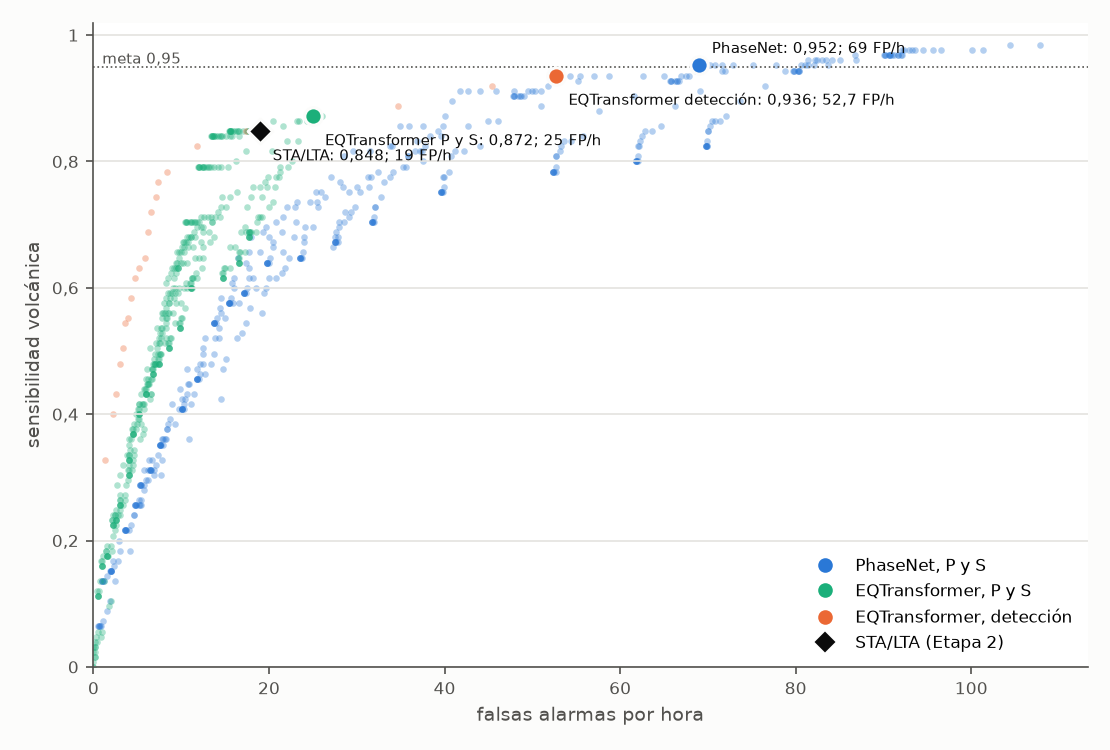
\includegraphics[width=0.85\textwidth]{figuras/fig9_costo_interseccion.png}
\caption{Sensibilidad volcánica contra falsas alarmas por hora. Cada punto es
una combinación de umbrales; los puntos grandes, la configuración elegida de
cada detector.}
\label{fig:res-costo}
\end{figure}

Con menos de 20 falsas alarmas por hora, EQTransformer con P y S y STA/LTA
llegan cerca de 0,85, más que PhaseNet con la misma cantidad de falsas
alarmas. Para pasar de ahí el costo sube rápido: solo PhaseNet supera 0,94, y
para llegar a 0,95 necesita 69,0 falsas alarmas por hora.

\subsection{Qué onda detecta cada evento}

Con \texttt{P\_threshold} en 0,40 y \texttt{S\_threshold} en 0,05, la onda S
sostiene casi toda la detección de PhaseNet: sola detecta 116 volcánicos
(0,928, con 73,3 falsas alarmas por hora), y la P sola, 72 (0,576, con 15,5).
El Cuadro~\ref{tab:res-onda} los separa por clase; ``solo P'' quiere decir que
la P detecta el evento y la S no.

{\small
\setlength{\tabcolsep}{3pt}
\begin{longtable}{lrrrrrrrr}
\caption{Volcánicos según la onda que los detecta, con la configuración de cada
red.}\label{tab:res-onda}\\
\cabecera{ & \multicolumn{4}{c}{\textbf{PhaseNet}} & \multicolumn{4}{c}{\textbf{EQTransformer}} \\ \textbf{Clase} & \textbf{Ambas} & \textbf{Solo P} & \textbf{Solo S} & \textbf{Ninguna} & \textbf{Ambas} & \textbf{Solo P} & \textbf{Solo S} & \textbf{Ninguna}}{9}
VT & 24 & 0 & 10 & 2 & 22 & 0 & 8 & 6 \\
LP & 31 & 1 & 18 & 2 & 36 & 1 & 10 & 5 \\
TR & 14 & 2 & 19 & 2 & 21 & 2 & 9 & 5 \\
\end{longtable}
}

En PhaseNet, la S detecta 47 volcánicos que la P no ve, y la P solo 3 que la S
no ve. Esto tiene un costo en el recorte, que empieza 2,5\,s antes del aviso:
cuando el aviso viene solo de la S, el recorte puede empezar después del
inicio del evento (Sección~\ref{sec:res-recorte}).

\subsection{Las dos redes juntas y las tres componentes}

Se juntaron las dos redes para ver si EQTransformer suma volcánicos que
PhaseNet no detecta. Los intervalos de PhaseNet y los de la curva de detección
de EQTransformer, cada uno con su configuración, se juntaron con la misma
regla que la P y la S: los que empiezan a 5\,s o menos del primero cuentan
como uno. Juntas detectan 122 de 125 volcánicos (0,976): 34 de 36 VT, 52 de 52
LP y 36 de 37 TR, con 101,0 falsas alarmas por hora. Frente a PhaseNet sola,
suman 2 LP y 1 TR, no pierden ninguno y cuestan 32 falsas alarmas por hora
más. El sistema usa solo PhaseNet.

Las dos redes esperan las tres componentes de la estación. Cuando solo se
tiene la vertical, una práctica posible es rellenar N y E con ceros. Con el
criterio anterior de 5\,s y umbral 0,10, esa opción baja a PhaseNet a 0,656 de
los volcánicos, contra 0,904 con Z, N y E reales; copiar la vertical en N y E
da 0,912. En EQTransformer, los ceros dan 0,624 y las tres componentes reales,
0,552. Las dos redes se usan con las tres componentes reales: aunque
EQTransformer rinde algo menos con ellas, así las dos reciben la misma señal.

% =====================================================================
\section{Calidad del recorte}
\label{sec:res-recorte}

El recorte por energía de PhaseNet (Sección~\ref{sec:recorte}) se comparó con
otras formas de delimitar los eventos, todas con la configuración elegida de
cada detector. La primera es el mismo recorte sin el último paso, el corte en
el aviso siguiente. La segunda es una ventana fija de 81,92\,s que empieza
2,5\,s antes del aviso de PhaseNet, el largo con que vienen cortados los
eventos del conjunto publicado por \textcite{espinosacurilem2025dataset}. Las
otras usan como recorte los intervalos que entregan STA/LTA y EQTransformer,
tal como salen de sus librerías y, como referencia, unidos cuando están a
menos de 5\,s uno de otro. Un evento queda bien recortado si su recorte tiene
un IoU de 0,3 o más con él.

{\footnotesize
\setlength{\tabcolsep}{3pt}
\begin{longtable}{>{\raggedright\arraybackslash}p{3.3cm}rrrrrrr}
\caption{Volcánicos bien recortados (IoU de 0,3 o más), IoU medio de esos
eventos, duración mediana de los recortes que tocan un volcánico (s) y
FP/h de la detección.}\label{tab:res-recortes}\\
\cabecera{\textbf{Recorte} & \textbf{VT} & \textbf{LP} & \textbf{TR} & \textbf{Volcánicos} & \textbf{IoU medio} & \textbf{Duración} & \textbf{FP/h}}{8}
PhaseNet + energía con corte & 35/36 & 49/52 & 24/37 & \textbf{108 = 0,864} & 0,68 & 22,0 & 69,0 \\
PhaseNet + energía & 34/36 & 37/52 & 27/37 & 98 = 0,784 & 0,69 & 31,8 & 69,0 \\
PhaseNet + ventana fija de 81,92\,s & 3/36 & 43/52 & 37/37 & 83 = 0,664 & 0,54 & 81,9 & 69,0 \\
STA/LTA, recorte propio & 28/36 & 34/52 & 4/37 & 66 = 0,528 & 0,46 & 11,2 & 19,0 \\
EQTransformer, recorte propio & 8/36 & 9/52 & 14/37 & 31 = 0,248 & 0,47 & 18,4 & 52,7 \\
\midrule
STA/LTA, unido a 5\,s & 28/36 & 34/52 & 6/37 & 68 = 0,544 & 0,46 & 11,5 & 19,0 \\
EQTransformer, unido a 5\,s & 11/36 & 10/52 & 15/37 & 36 = 0,288 & 0,48 & 20,4 & 52,7 \\
\end{longtable}
}

El mejor es el recorte por energía con corte: 108 de 125 volcánicos bien
recortados (0,864). La ventana fija solo gana en TR, porque con 81,92\,s cubre
casi cualquier evento largo; en VT, que duran unos 12\,s, acierta 3 de 36.
STA/LTA pierde casi todos los TR (4 de 37). Los recortes de EQTransformer duran
18,4\,s en mediana, y los eventos, 32,6\,s, así que se quedan cortos: recorta
bien solo 31 volcánicos. Unir los intervalos a 5\,s cambia poco: 2 eventos más
en STA/LTA y 5 en EQTransformer.

El corte en el aviso siguiente se agregó porque, sin él, muchos recortes
salían demasiado largos: con eventos seguidos, el recorte se tragaba al
siguiente (Figura~\ref{fig:res-fallas}, arriba). El corte sube LP de 37 a 49,
pero baja TR de 27 a 24, probablemente porque PhaseNet da varios avisos dentro
de un mismo tremor. Además, con umbral 0,10 se vio que 6 TR quedan cortos
porque en FRE casi no sobresalen del ruido: su energía llega solo a entre 0,8 y
1,6 veces el nivel del ruido (Figura~\ref{fig:res-fallas}, abajo). La
Figura~\ref{fig:res-ejemplos} muestra un caso típico de cada clase.

\begin{figure}[!ht]
\centering
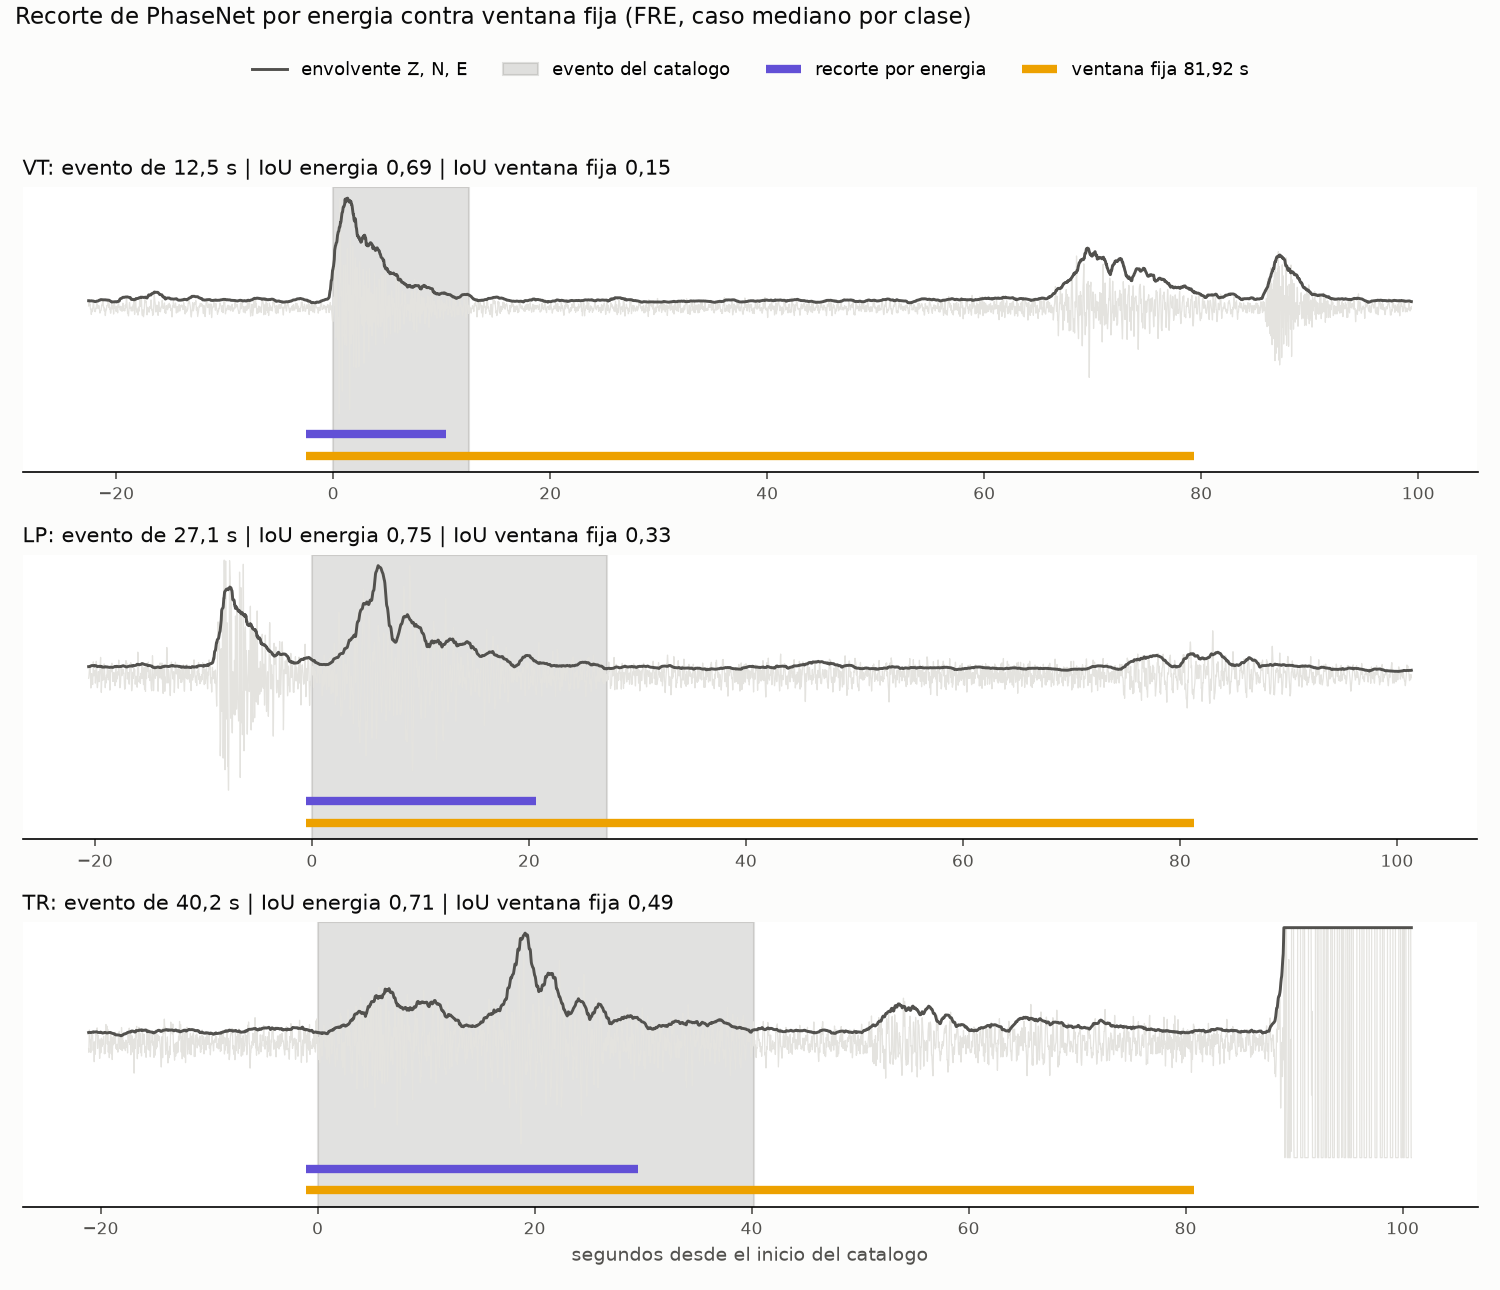
\includegraphics[width=0.78\textwidth]{figuras/fig5_recortes.png}
\caption{Recorte por energía, sin el corte en el aviso siguiente, y ventana
fija en un caso típico de cada clase volcánica, con los avisos de PhaseNet en
umbral 0,10. En el panel de TR, desde los 89\,s aparece una señal mucho mayor
que sale de la escala.}
\label{fig:res-ejemplos}
\end{figure}

\begin{figure}[!ht]
\centering
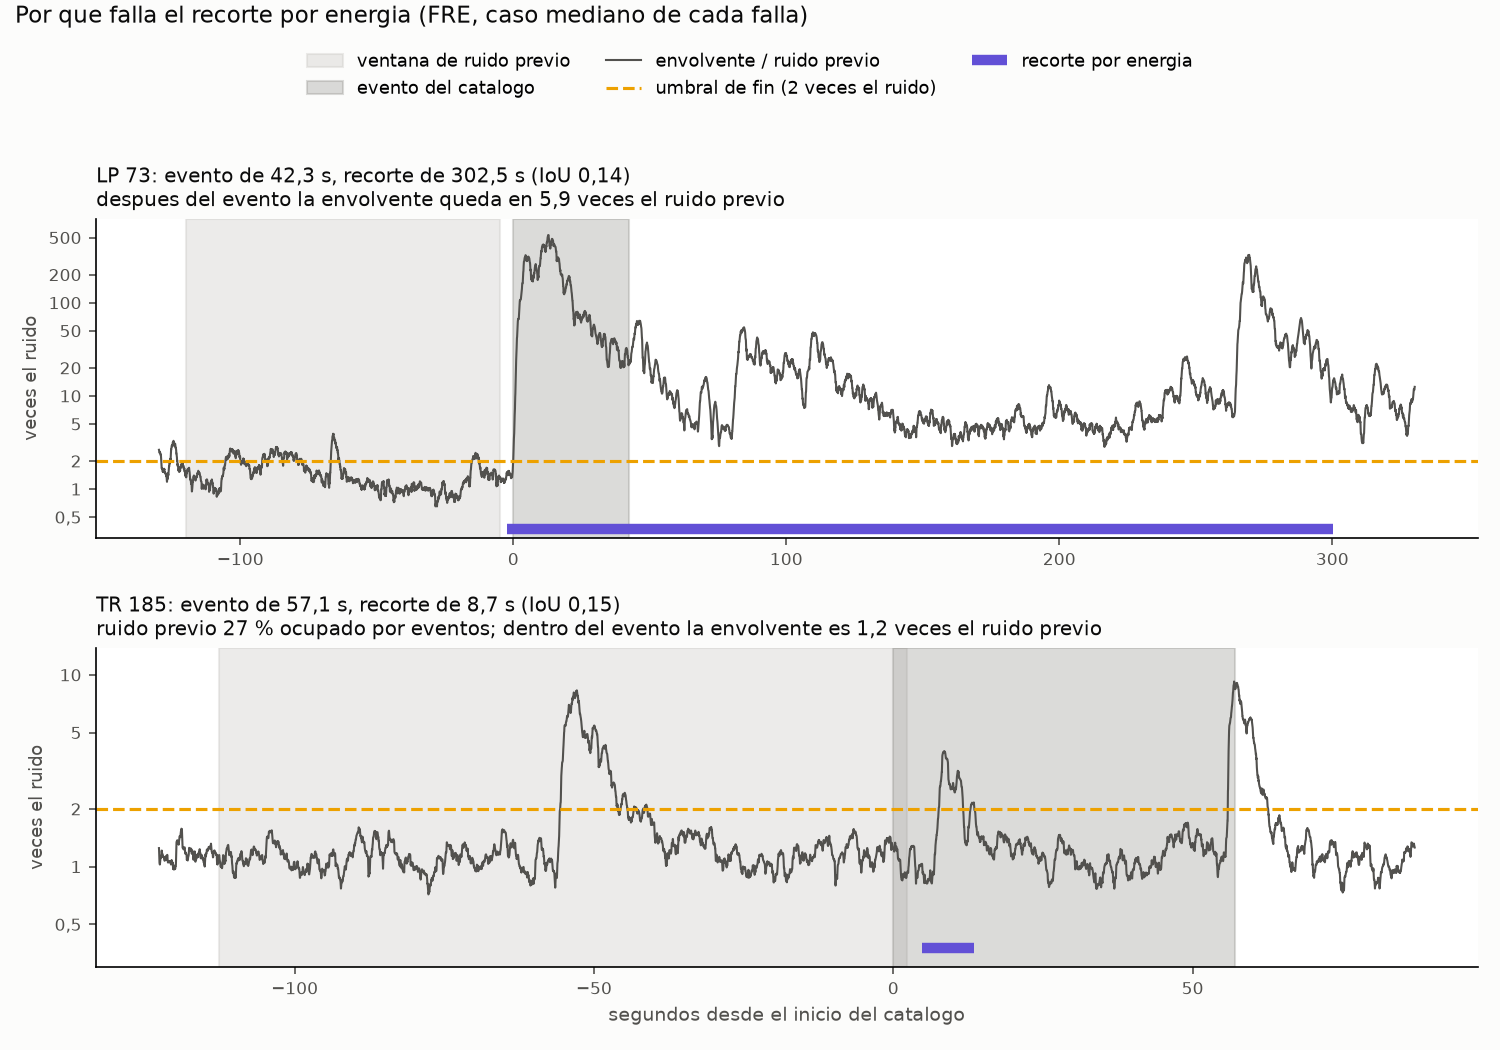
\includegraphics[width=0.80\textwidth]{figuras/fig6_fallas.png}
\caption{Dos fallas del recorte por energía, con los avisos de PhaseNet en
umbral 0,10: un LP con recorte demasiado largo y un TR con recorte demasiado
corto. La energía está medida en veces el ruido previo; el recorte termina
cuando baja de la línea punteada durante 5\,s.}
\label{fig:res-fallas}
\end{figure}

\subsection{Calidad con varios umbrales de IoU}

El umbral de 0,3 es una decisión propia de este trabajo, así que se contó
también cuántos volcánicos tienen un recorte que los toca y cuántos superan
cada umbral de IoU, de 0,1 a 0,9 (Cuadro~\ref{tab:res-iou} y
Figura~\ref{fig:res-iou}).

{\small
\setlength{\tabcolsep}{3pt}
\begin{longtable}{>{\raggedright\arraybackslash}p{5.0cm}rrrrrrrrrr}
\caption{Volcánicos, de 125, con un recorte que los toca y con IoU igual o
mayor que cada umbral.}\label{tab:res-iou}\\
\cabecera{\textbf{Recorte} & \textbf{Toca} & \textbf{0,1} & \textbf{0,2} & \textbf{0,3} & \textbf{0,4} & \textbf{0,5} & \textbf{0,6} & \textbf{0,7} & \textbf{0,8} & \textbf{0,9}}{11}
PhaseNet + energía con corte & 122 & 120 & 112 & 108 & 102 & 87 & 69 & 49 & 32 & 14 \\
PhaseNet + energía & 120 & 120 & 105 & 98 & 94 & 83 & 69 & 49 & 29 & 13 \\
PhaseNet + ventana fija de 81,92\,s & 125 & 124 & 101 & 83 & 60 & 39 & 22 & 17 & 10 & 5 \\
EQTransformer, recorte propio & 117 & 105 & 68 & 31 & 18 & 10 & 5 & 4 & 1 & 0 \\
STA/LTA, recorte propio & 106 & 100 & 90 & 66 & 39 & 20 & 14 & 5 & 2 & 0 \\
\end{longtable}
}

\begin{figure}[!ht]
\centering
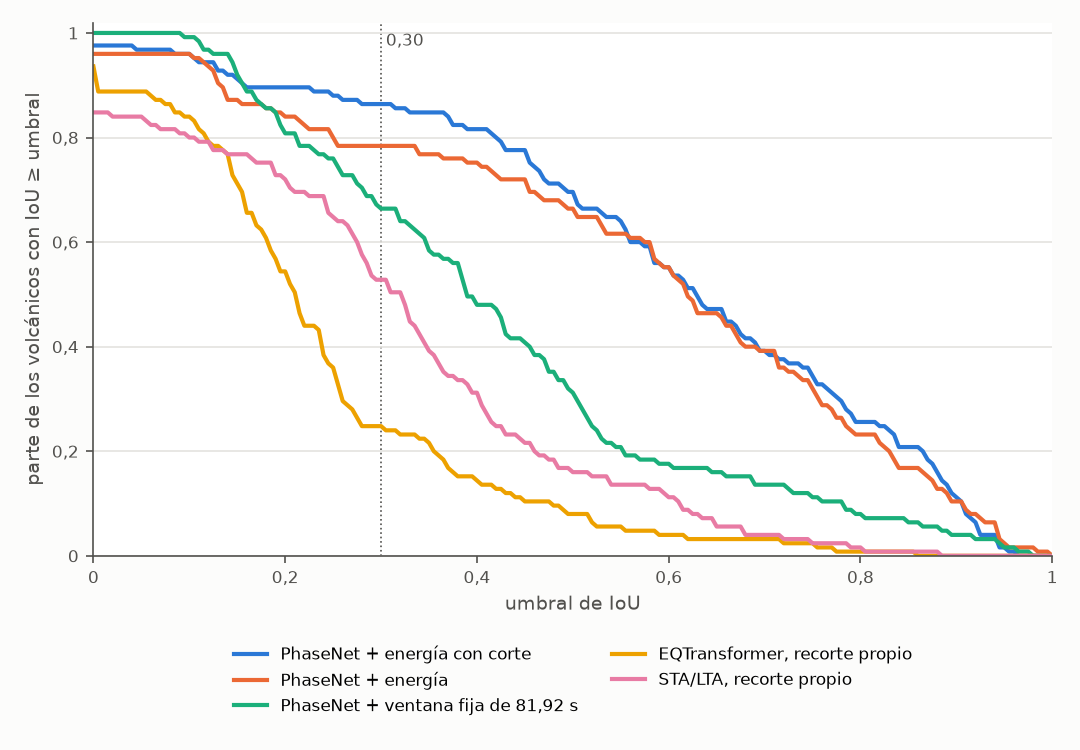
\includegraphics[width=0.80\textwidth]{figuras/fig7_iou.png}
\caption{Parte de los 125 volcánicos con IoU igual o mayor que cada umbral,
para cada recorte. La línea punteada marca el umbral de 0,3.}
\label{fig:res-iou}
\end{figure}

Tocar el evento no basta. Si se cuenta todo recorte que lo toca, el recorte
por energía con corte llega a 122 de 125 (0,976) y la ventana fija toca los
125, pero los toca porque es larga: en VT su IoU mediano es 0,19. Con IoU de
0,5 o más, el recorte por energía con corte delimita bien 87 volcánicos
(0,696); sin corte, 83; la ventana fija, 39; STA/LTA, 20, y EQTransformer, 10.
El Cuadro~\ref{tab:res-iou-clase} separa por clase.

{\small
\setlength{\tabcolsep}{4pt}
\begin{longtable}{>{\raggedright\arraybackslash}p{5.0cm}lrrrrr}
\caption{Por clase: eventos con un recorte que los toca y con IoU de 0,3, 0,5
y 0,7 o más, e IoU mediano de los que se tocan.}\label{tab:res-iou-clase}\\
\cabecera{\textbf{Recorte} & \textbf{Clase} & \textbf{Toca} & \textbf{0,3} & \textbf{0,5} & \textbf{0,7} & \textbf{Mediana}}{7}
PhaseNet + energía con corte & VT (36) & 35 & 35 & 33 & 18 & 0,71 \\
 & LP (52) & 51 & 49 & 40 & 24 & 0,67 \\
 & TR (37) & 36 & 24 & 14 & 7 & 0,44 \\
\midrule
PhaseNet + energía & VT (36) & 35 & 34 & 32 & 17 & 0,69 \\
 & LP (52) & 50 & 37 & 28 & 18 & 0,56 \\
 & TR (37) & 35 & 27 & 23 & 14 & 0,62 \\
\midrule
PhaseNet + ventana fija de 81,92\,s & VT (36) & 36 & 3 & 0 & 0 & 0,19 \\
 & LP (52) & 52 & 43 & 13 & 0 & 0,41 \\
 & TR (37) & 37 & 37 & 26 & 17 & 0,69 \\
\midrule
EQTransformer, recorte propio & VT (36) & 30 & 8 & 0 & 0 & 0,24 \\
 & LP (52) & 52 & 9 & 2 & 0 & 0,20 \\
 & TR (37) & 35 & 14 & 8 & 4 & 0,26 \\
\midrule
STA/LTA, recorte propio & VT (36) & 32 & 28 & 13 & 4 & 0,46 \\
 & LP (52) & 45 & 34 & 5 & 1 & 0,36 \\
 & TR (37) & 29 & 4 & 2 & 0 & 0,19 \\
\end{longtable}
}

Con el recorte por energía con corte, VT y LP quedan bien delimitados (IoU
mediano de 0,71 y 0,67) y TR es lo más débil (0,44). En TR rinden mejor el
mismo recorte sin corte (0,62) y la ventana fija (0,69), porque el tremor es
largo.

\subsection{Cómo falla el recorte}

Cuando un recorte toca su evento, puede hacerlo de cuatro formas: cubrirlo
entero, empezando antes y terminando después; empezar antes y terminar dentro
del evento, de modo que le falta el final; quedar dentro del evento, de modo
que le faltan el inicio y el fin; o empezar dentro del evento y terminar
después, de modo que le falta el inicio. El Cuadro~\ref{tab:res-casos} cuenta
cuántos volcánicos caen en cada caso; cada fila suma 125.

{\footnotesize
\setlength{\tabcolsep}{3pt}
\begin{longtable}{>{\raggedright\arraybackslash}p{3.0cm}>{\raggedleft\arraybackslash}p{1.8cm}>{\raggedleft\arraybackslash}p{1.8cm}>{\raggedleft\arraybackslash}p{1.8cm}>{\raggedleft\arraybackslash}p{1.8cm}>{\raggedleft\arraybackslash}p{1.8cm}}
\caption{Volcánicos según cómo los toca su recorte; entre paréntesis, IoU
mediano.}\label{tab:res-casos}\\
\cabecera{\textbf{Recorte} & \textbf{Cubre todo} & \textbf{Falta el final} & \textbf{Faltan inicio y fin} & \textbf{Falta el inicio} & \textbf{No lo toca}}{6}
PhaseNet + energía con corte & 26 (0,72) & 46 (0,71) & 36 (0,53) & 14 (0,68) & 3 \\
PhaseNet + energía & 37 (0,53) & 40 (0,74) & 20 (0,60) & 23 (0,62) & 5 \\
PhaseNet + ventana fija de 81,92\,s & 91 (0,34) & 5 (0,64) & 17 (0,66) & 12 (0,53) & 0 \\
EQTransformer, recorte propio & 5 (0,49) & 65 (0,24) & 40 (0,17) & 7 (0,43) & 8 \\
STA/LTA, recorte propio & 0 & 13 (0,40) & 92 (0,33) & 1 (0,52) & 19 \\
\end{longtable}
}

El recorte por energía con corte falla sobre todo por el final: en 82
volcánicos termina antes que el evento (46 más 36), y en 50 empieza después
del inicio que marca el catálogo (36 más 14). STA/LTA corta corto: en 92 casos
su recorte queda dentro del evento. EQTransformer suele empezar antes del
evento y terminar antes de su fin.

Que el recorte empiece tarde depende de qué onda dio el aviso. Como la onda S
llega después de la P, cuando PhaseNet solo ve la S el margen de 2,5\,s puede
no alcanzar. El Cuadro~\ref{tab:res-inicio} lo mide para cada volcánico que su
recorte toca.

{\small
\setlength{\tabcolsep}{4pt}
\begin{longtable}{llr>{\raggedleft\arraybackslash}p{1.7cm}>{\raggedleft\arraybackslash}p{1.9cm}>{\raggedleft\arraybackslash}p{2.8cm}>{\raggedleft\arraybackslash}p{1.7cm}}
\caption{Inicio del recorte por energía con corte según la onda que dio el
aviso.}\label{tab:res-inicio}\\
\cabecera{\textbf{Onda} & \textbf{Clase} & \textbf{Eventos} & \textbf{Empieza antes} & \textbf{Empieza después} & \textbf{Aviso tras el inicio, mediana (s)} & \textbf{IoU mediano}}{7}
P & VT & 28 & 23 & 5 & 1,5 & 0,73 \\
P & LP & 35 & 26 & 9 & 1,6 & 0,69 \\
P & TR & 7 & 6 & 1 & 0,8 & 0,50 \\
P & Todas & 70 & 55 & 15 & 1,6 & 0,72 \\
\midrule
S & VT & 7 & 6 & 1 & 0,0 & 0,61 \\
S & LP & 16 & 7 & 9 & 2,8 & 0,64 \\
S & TR & 29 & 4 & 25 & 12,9 & 0,42 \\
S & Todas & 52 & 17 & 35 & 4,4 & 0,55 \\
\end{longtable}
}

Cuando avisa la P, el recorte empieza antes del inicio en 55 de 70 casos: el
aviso llega en mediana 1,6\,s después del inicio, dentro del margen de 2,5\,s.
Cuando el aviso viene de la S, el recorte empieza después del inicio en 35 de 52
casos, porque la S llega en mediana 4,4\,s después; en esos casos el recorte
pierde la onda P. Casi todos son TR: en 25 de los 29 TR avisados por la S, el
recorte empieza tarde, con el aviso 12,9\,s después del inicio en
mediana. Bajar \texttt{P\_threshold} casi no lo corrige: con 0,02, en 4 de los
21 recortes que empezaban tarde con 0,10 para las dos ondas el aviso pasa a
venir de la P, pero solo 1 empieza antes del inicio. En estos eventos, casi
todos TR, PhaseNet no marca una onda P temprana ni con umbrales muy bajos.

% =====================================================================
\section{Detección y recorte en las ventanas de test}
\label{sec:res-deteccion-test}

La misma detección y el mismo recorte, con la configuración elegida, se
aplicaron a las 1.161 ventanas de test, que no se usaron para elegir ningún
parámetro. Cada ventana tiene su evento principal al centro, así que se cuenta
cuántos de esos eventos se detectan y cuántos quedan con un recorte de IoU de
0,3 o más (Cuadro~\ref{tab:res-test-deteccion}).

\needspace{9\baselineskip}
{\footnotesize
\setlength{\tabcolsep}{3pt}
\begin{longtable}{lrrlrl}
\caption{Detección y recorte del evento principal de las ventanas de test.
Entre corchetes, el intervalo de confianza del 95\,\%.}\label{tab:res-test-deteccion}\\
\cabecera{\textbf{Clase} & \textbf{Eventos} & \textbf{Detectados} & \textbf{Sensibilidad} & \textbf{IoU $\geq$ 0,3} & \textbf{Parte}}{6}
VT & 300 & 300 & 1,000 [0,987; 1,000] & 293 & 0,977 [0,953; 0,989] \\
LP & 288 & 278 & 0,965 [0,937; 0,981] & 281 & 0,976 [0,951; 0,988] \\
TR & 281 & 267 & 0,950 [0,918; 0,970] & 183 & 0,651 [0,594; 0,705] \\
\midrule
\textbf{Volcánicos} & \textbf{869} & \textbf{845} & \textbf{0,972 [0,959; 0,981]} & \textbf{757} & \textbf{0,871 [0,847; 0,892]} \\
\end{longtable}
}

La sensibilidad de detección y la parte bien recortada son parecidas a las de
la traza continua (0,972 contra 0,952 y 0,871 contra 0,864), y en las dos TR es
la clase peor recortada: 0,651 en test y 24 de 37 (0,649) en la traza. En LP
hay más eventos bien recortados (281) que detectados (278), porque la
detección se cuenta con los intervalos de los avisos, que son cortos, y el
recorte, que es más largo, puede tocar un evento cuyo aviso no lo tocó.

En las 1.161 ventanas, que suman 96,75 horas, la detección y el recorte
producen 7.621 recortes, 6,6 por ventana. Los que no quedan emparejados con
ninguna caja del catálogo son 59,5 por hora, el 75,6\,\% de todos los recortes.
Detectar y recortar una ventana de 300\,s toma 0,02\,s en el procesador del
computador, sin tarjeta gráfica.

% =====================================================================
\section{Clasificador}
\label{sec:res-clasificador}

\subsection{Búsqueda de la configuración}
\label{subsec:res-busqueda}

La búsqueda hizo 20 pruebas por red, entrenando con los folds 2 a 5 y
validando con el fold 1 (Sección~\ref{subsec:busqueda}). El
Cuadro~\ref{tab:res-busqueda} muestra la combinación con mayor F1 macro de VT,
LP y TR en validación para cada red.

{\small
\setlength{\tabcolsep}{4pt}
\begin{longtable}{>{\raggedright\arraybackslash}p{3.2cm}>{\raggedright\arraybackslash}p{3.0cm}>{\raggedright\arraybackslash}p{3.0cm}>{\raggedright\arraybackslash}p{3.0cm}}
\caption{Mejor combinación de cada red en la búsqueda (fold 1 de
validación).}\label{tab:res-busqueda}\\
\cabecera{\textbf{Parámetro} & \textbf{EfficientNet-B0} & \textbf{ResNet50} & \textbf{VGG16}}{4}
Optimizador & AdamW & SGD con momentum 0,9 & AdamW \\
Tasa de aprendizaje & 0,001 & 0,01 & 0,00001 \\
Dropout & 0,3 & 0,3 & 0,3 \\
Tamaño de lote & 16 & 32 & 16 \\
Weight decay & 0 & 0 & 0,0001 \\
Función de pérdida & Focal & Entropía cruzada con pesos & Entropía cruzada con pesos \\
\midrule
F1 macro de VT, LP y TR en validación & 0,866 & 0,859 & 0,856 \\
\end{longtable}
}

Las tres redes quedan con dropout 0,3, el mayor de los dos probados, y cada una
con una tasa de aprendizaje distinta. Entre la mejor y la peor hay 0,010 de F1
macro, menos que la variación entre folds de una misma red que se ve más
adelante.

Para ver cuánto aportan la búsqueda, el aumento de datos y la parada temprana,
el Cuadro~\ref{tab:res-antes} compara cada red, en el mismo fold de
validación, con una configuración inicial sin ellos: AdamW con tasa de
aprendizaje 0,0001, 10 épocas y sin aumento de datos.

\needspace{9\baselineskip}
{\small
\begin{longtable}{lrrr}
\caption{F1 macro de VT, LP y TR en el fold 1 de validación, con la
configuración inicial y con la elegida.}\label{tab:res-antes}\\
\cabecera{\textbf{Red} & \textbf{Inicial} & \textbf{Elegida} & \textbf{Diferencia}}{4}
EfficientNet-B0 & 0,834 & 0,866 & +0,032 \\
ResNet50 & 0,835 & 0,859 & +0,024 \\
VGG16 & 0,835 & 0,856 & +0,021 \\
\end{longtable}
}

La mejora es de 0,02 a 0,03 en las tres redes. Por clase, la sensibilidad de
VT sube de entre 0,89 y 0,92 a entre 0,92 y 0,95, y la de TR queda parecida
(de entre 0,78 y 0,81 a entre 0,75 y 0,82). Como se mide en una sola partición,
la mejora es del mismo orden que la variación entre folds.

\subsection{Validación cruzada y test}
\label{subsec:res-folds}

Con la combinación elegida, cada red se entrenó cinco veces, una por fold de
validación, y el mejor modelo de cada vez se evaluó en las 1.161 ventanas de
test. En test hay 336 recortes VT, 676 LP, 244 TR y 320 de rechazo con IoU de
0,3 o más y 5\,s o más de duración. El Cuadro~\ref{tab:res-f1} resume el F1 macro de VT, LP y TR de los
cinco modelos, con el recorte y con la ventana fija de 60\,s.

\needspace{9\baselineskip}
{\small
\setlength{\tabcolsep}{4pt}
\begin{longtable}{>{\raggedright\arraybackslash}p{2.6cm}>{\raggedright\arraybackslash}p{2.0cm}>{\raggedright\arraybackslash}p{3.2cm}>{\raggedright\arraybackslash}p{3.2cm}}
\caption{F1 macro de VT, LP y TR de los cinco modelos de cada red: promedio
y desviación estándar y, debajo, mínimo y máximo entre corchetes.}\label{tab:res-f1}\\
\cabecera{\textbf{Red} & \textbf{Entrada} & \textbf{Validación} & \textbf{Test}}{4}
EfficientNet-B0 & Recorte & 0,871 $\pm$ 0,007 \newline [0,864; 0,880] & 0,840 $\pm$ 0,009 \newline [0,828; 0,848] \\
 & Fija de 60\,s & 0,862 $\pm$ 0,013 \newline [0,846; 0,877] & 0,835 $\pm$ 0,006 \newline [0,828; 0,844] \\
\midrule
ResNet50 & Recorte & 0,865 $\pm$ 0,007 \newline [0,859; 0,876] & 0,834 $\pm$ 0,012 \newline [0,823; 0,853] \\
 & Fija de 60\,s & 0,860 $\pm$ 0,014 \newline [0,842; 0,879] & 0,831 $\pm$ 0,003 \newline [0,826; 0,835] \\
\midrule
VGG16 & Recorte & 0,866 $\pm$ 0,014 \newline [0,856; 0,891] & 0,843 $\pm$ 0,008 \newline [0,833; 0,853] \\
 & Fija de 60\,s & 0,855 $\pm$ 0,008 \newline [0,843; 0,861] & 0,834 $\pm$ 0,009 \newline [0,825; 0,847] \\
\end{longtable}
}

En test, el F1 macro con el recorte va de 0,834 a 0,843 según la red, entre
0,02 y 0,03 menos que en validación. Esa diferencia es esperable, porque la
validación se usa para elegir la época y, en el fold 1, la configuración. Las
diferencias entre redes, de hasta 0,009, son menores que la distancia entre
el mejor y el peor de los cinco modelos de una misma red, que llega a 0,030;
con estos datos ninguna de las tres redes supera claramente a las otras. La
ventana fija de 60\,s queda entre 0,831 y 0,835.

Los Cuadros~\ref{tab:res-clases-recorte} y~\ref{tab:res-clases-fija} separan
por clase la sensibilidad y el F1 en test.

{\small
\setlength{\tabcolsep}{4pt}
\begin{longtable}{>{\raggedright\arraybackslash}p{2.0cm}>{\raggedright\arraybackslash}p{3.4cm}>{\raggedright\arraybackslash}p{3.4cm}>{\raggedright\arraybackslash}p{3.4cm}}
\caption{Test con el recorte: sensibilidad por clase, con mínimo y máximo de
los cinco modelos entre corchetes, y F1 promedio.}\label{tab:res-clases-recorte}\\
\cabecera{\textbf{Clase} & \textbf{EfficientNet-B0} & \textbf{ResNet50} & \textbf{VGG16}}{4}
\multicolumn{4}{l}{\textit{Sensibilidad}}\\*
VT & 0,893 [0,875; 0,908] & 0,910 [0,881; 0,949] & 0,889 [0,854; 0,920] \\
LP & 0,869 [0,837; 0,895] & 0,812 [0,780; 0,870] & 0,834 [0,812; 0,852] \\
TR & 0,764 [0,734; 0,840] & 0,831 [0,787; 0,877] & 0,811 [0,803; 0,824] \\
Rechazo & 0,853 [0,791; 0,916] & 0,857 [0,769; 0,909] & 0,904 [0,875; 0,928] \\
\midrule
\multicolumn{4}{l}{\textit{F1}}\\*
VT & 0,854 & 0,841 & 0,848 \\
LP & 0,872 & 0,855 & 0,867 \\
TR & 0,794 & 0,805 & 0,815 \\
Rechazo & 0,861 & 0,861 & 0,875 \\
\end{longtable}
}

{\small
\setlength{\tabcolsep}{4pt}
\begin{longtable}{>{\raggedright\arraybackslash}p{2.0cm}>{\raggedright\arraybackslash}p{3.4cm}>{\raggedright\arraybackslash}p{3.4cm}>{\raggedright\arraybackslash}p{3.4cm}}
\caption{Test con la ventana fija de 60\,s: sensibilidad por clase, con mínimo
y máximo de los cinco modelos entre corchetes, y F1 promedio.}\label{tab:res-clases-fija}\\
\cabecera{\textbf{Clase} & \textbf{EfficientNet-B0} & \textbf{ResNet50} & \textbf{VGG16}}{4}
\multicolumn{4}{l}{\textit{Sensibilidad}}\\*
VT & 0,907 [0,860; 0,940] & 0,901 [0,866; 0,932] & 0,900 [0,884; 0,926] \\
LP & 0,856 [0,818; 0,889] & 0,824 [0,808; 0,836] & 0,843 [0,780; 0,892] \\
TR & 0,761 [0,721; 0,803] & 0,777 [0,738; 0,807] & 0,782 [0,742; 0,844] \\
Rechazo & 0,831 [0,766; 0,884] & 0,880 [0,816; 0,916] & 0,855 [0,828; 0,888] \\
\midrule
\multicolumn{4}{l}{\textit{F1}}\\*
VT & 0,849 & 0,846 & 0,854 \\
LP & 0,860 & 0,854 & 0,860 \\
TR & 0,795 & 0,792 & 0,787 \\
Rechazo & 0,856 & 0,862 & 0,862 \\
\end{longtable}
}

VT es la clase que mejor se reconoce en las tres redes, con sensibilidades
entre 0,889 y 0,910 con el recorte. TR es la más difícil: entre 0,764 y 0,831.
La Figura~\ref{fig:res-matrices-test} muestra con qué se confunde cada clase.
TR va a LP entre el 13 y el 21\,\% de las veces con el recorte, y del rechazo
entre el 6 y el 10\,\% va a VT. VT y TR casi nunca se confunden entre sí: menos
del 1\,\% en cualquier sentido.

\begin{figure}[!ht]
\centering
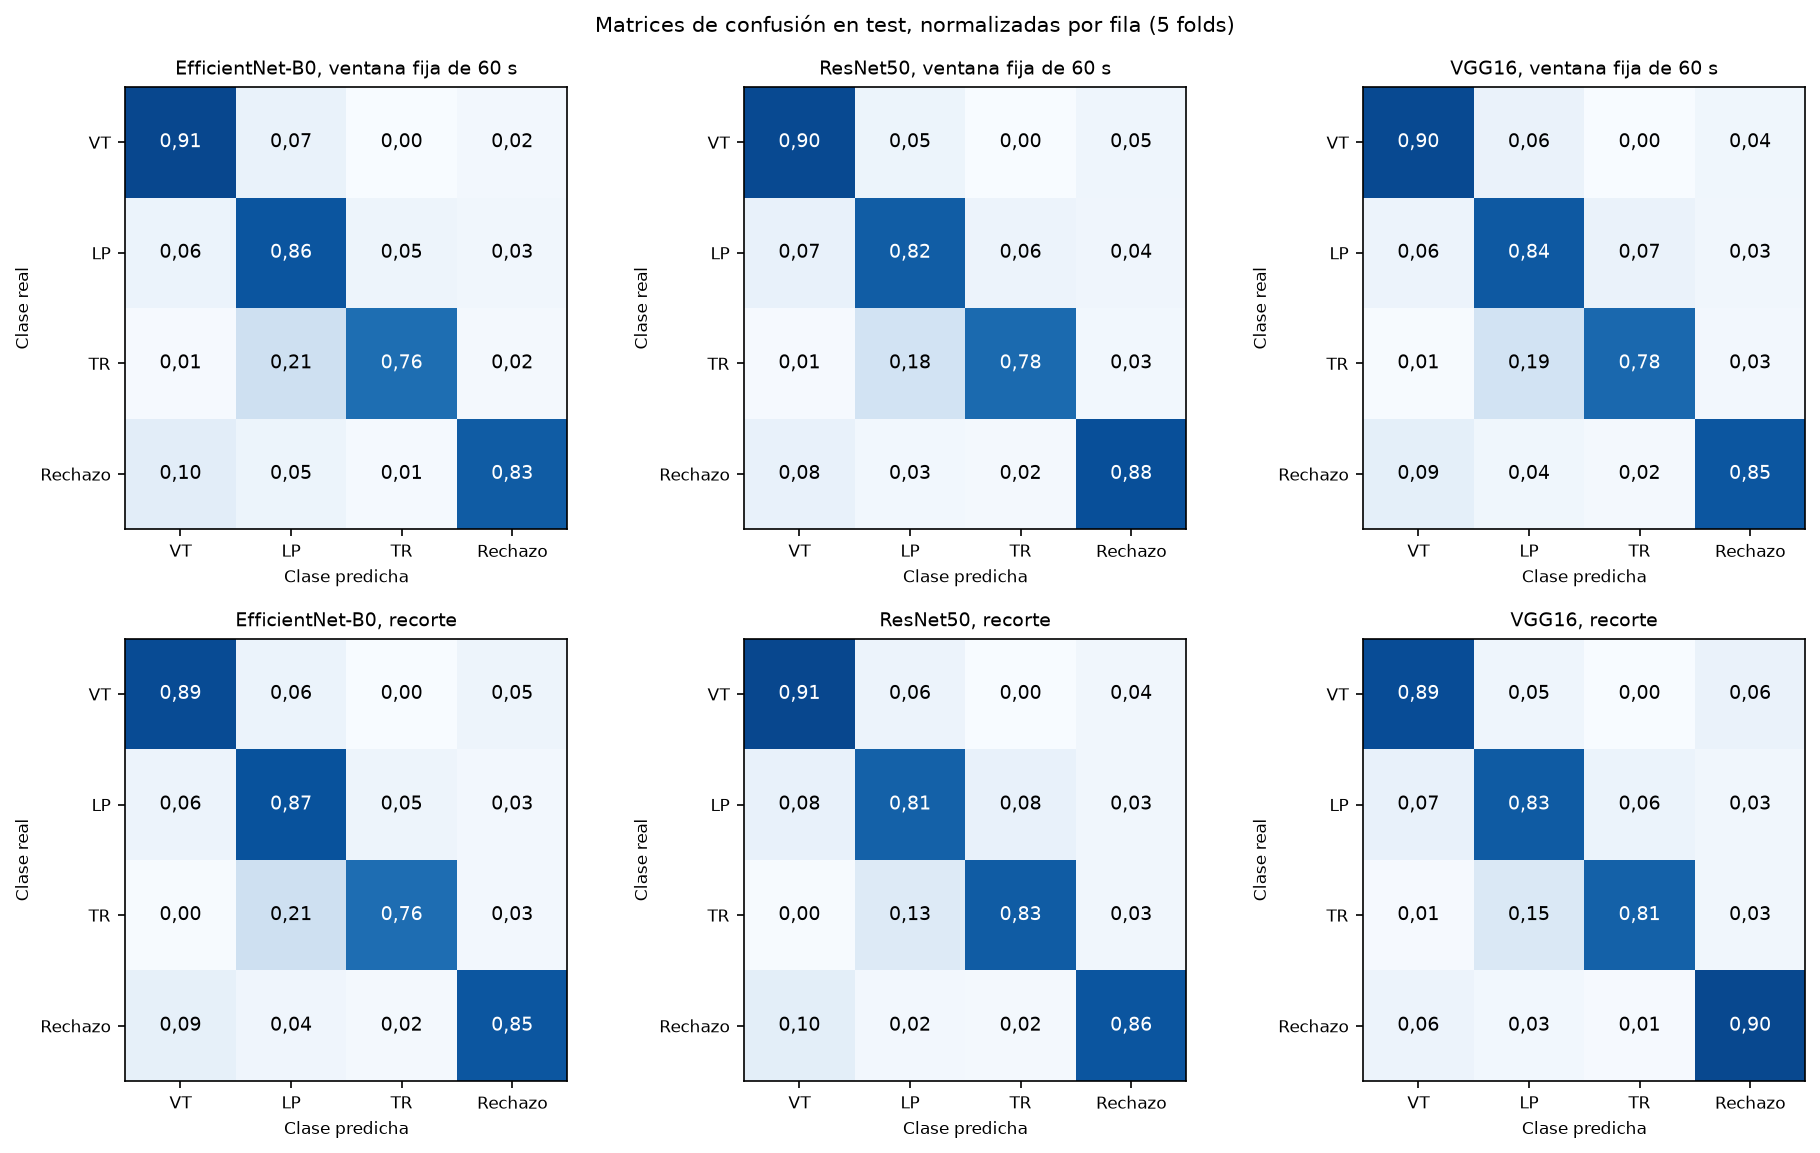
\includegraphics[width=\textwidth]{images/matrices_test.png}
\caption{Matrices de confusión en test, normalizadas por fila (suma de los
cinco modelos de cada red). Arriba, con la ventana fija de 60\,s; abajo, con el
recorte.}
\label{fig:res-matrices-test}
\end{figure}

Los recortes sin caja no se usan para entrenar ni en las métricas anteriores,
pero se clasifican igual, porque en operación el sistema los recibe. En test
hay 2.420 recortes sin caja de 5\,s o más. Con el recorte, EfficientNet-B0
clasifica como volcánicos al 75,0\,\%, ResNet50 al 76,1\,\% y VGG16 al
74,7\,\%; con la ventana fija, al 78,3, 65,8 y 74,7\,\%. El clasificador, que
solo aprendió a separar VT, LP y TR de AV e IC, manda a la clase de rechazo
entre una cuarta y una tercera parte de estos recortes.

% =====================================================================
\section{Sistema completo sobre la traza continua}
\label{sec:res-sistema}

La cadena completa se aplicó a las 9,74 horas válidas de la traza continua de
FRE, con los cinco modelos de cada red. La detección y el recorte dan 1.155
recortes, que se etiquetan contra el catálogo con la misma regla que los de las
ventanas etiquetadas (Cuadro~\ref{tab:res-traza-etiquetas}).

{\small
\begin{longtable}{lr}
\caption{Recortes de la traza continua por etiqueta.}\label{tab:res-traza-etiquetas}\\
\cabecera{\textbf{Etiqueta} & \textbf{Recortes}}{2}
VT & 35 \\
LP & 50 \\
TR & 24 \\
AV & 6 \\
IC & 34 \\
Fuera (tocan un evento con IoU menor que 0,3) & 151 \\
Sin caja (no tocan ningún evento) & 855 \\
\midrule
Total & 1.155 \\
\end{longtable}
}

\subsection{Clasificación y sensibilidad completa}
\label{subsec:res-sistema-clases}

Los 109 recortes volcánicos con IoU de 0,3 o más corresponden a 35 de los 36
VT, 50 de los 52 LP y 24 de los 37 TR. Eso pone un techo a la sensibilidad
completa, la parte de los eventos que el sistema detecta, recorta y clasifica
bien a la vez: aunque el clasificador acertara todos los recortes, el sistema
llegaría a 0,972 en VT, 0,962 en LP, 0,649 en TR y 0,872 en los volcánicos.
El Cuadro~\ref{tab:res-sistema} da los resultados con el recorte y el
Cuadro~\ref{tab:res-sistema-fija}, con la ventana fija de 60\,s. Cada cifra
es el promedio de los cinco modelos de cada red; junto al F1 macro y a la
sensibilidad completa volcánica va la desviación estándar.

{\small
\setlength{\tabcolsep}{4pt}
\begin{longtable}{>{\raggedright\arraybackslash}p{4.0cm}>{\raggedright\arraybackslash}p{2.7cm}>{\raggedright\arraybackslash}p{2.7cm}>{\raggedright\arraybackslash}p{2.7cm}}
\caption{Sistema completo en la traza continua, con el recorte. Entre
paréntesis, cuántos recortes o eventos entran en cada cifra.}\label{tab:res-sistema}\\
\cabecera{\textbf{Medida} & \textbf{EfficientNet-B0} & \textbf{ResNet50} & \textbf{VGG16}}{4}
\multicolumn{4}{l}{\textit{Clasificación de los recortes con IoU de 0,3 o más}}\\*
F1 macro de VT, LP y TR & 0,717 $\pm$ 0,023 & 0,770 $\pm$ 0,029 & 0,719 $\pm$ 0,037 \\
Sensibilidad VT (35) & 0,594 & 0,691 & 0,583 \\
Sensibilidad LP (50) & 0,932 & 0,892 & 0,872 \\
Sensibilidad TR (24) & 0,667 & 0,800 & 0,700 \\
Sensibilidad rechazo (40) & 0,465 & 0,540 & 0,595 \\
\midrule
\multicolumn{4}{l}{\textit{Sensibilidad completa}}\\*
VT (36) & 0,578 & 0,672 & 0,567 \\
LP (52) & 0,896 & 0,858 & 0,838 \\
TR (37) & 0,432 & 0,519 & 0,454 \\
Volcánicos (125) & 0,667 $\pm$ 0,012 & 0,704 $\pm$ 0,020 & 0,646 $\pm$ 0,031 \\
AV (6) & 0,533 & 0,467 & 0,400 \\
IC (48) & 0,321 & 0,392 & 0,446 \\
\midrule
Recortes sin caja clasificados como volcánicos, por hora & 67,9 & 64,5 & 60,0 \\
\end{longtable}
}

{\small
\setlength{\tabcolsep}{4pt}
\begin{longtable}{>{\raggedright\arraybackslash}p{4.0cm}>{\raggedright\arraybackslash}p{2.7cm}>{\raggedright\arraybackslash}p{2.7cm}>{\raggedright\arraybackslash}p{2.7cm}}
\caption{Sistema completo en la traza continua, con la ventana fija de
60\,s.}\label{tab:res-sistema-fija}\\
\cabecera{\textbf{Medida} & \textbf{EfficientNet-B0} & \textbf{ResNet50} & \textbf{VGG16}}{4}
\multicolumn{4}{l}{\textit{Clasificación de los recortes con IoU de 0,3 o más}}\\*
F1 macro de VT, LP y TR & 0,710 $\pm$ 0,028 & 0,708 $\pm$ 0,038 & 0,720 $\pm$ 0,013 \\
Sensibilidad VT (35) & 0,680 & 0,680 & 0,743 \\
Sensibilidad LP (50) & 0,904 & 0,836 & 0,860 \\
Sensibilidad TR (24) & 0,625 & 0,642 & 0,642 \\
Sensibilidad rechazo (40) & 0,470 & 0,600 & 0,510 \\
\midrule
\multicolumn{4}{l}{\textit{Sensibilidad completa}}\\*
VT (36) & 0,661 & 0,661 & 0,722 \\
LP (52) & 0,869 & 0,804 & 0,827 \\
TR (37) & 0,405 & 0,416 & 0,416 \\
Volcánicos (125) & 0,672 $\pm$ 0,020 & 0,648 $\pm$ 0,032 & 0,675 $\pm$ 0,009 \\
AV (6) & 0,467 & 0,767 & 0,567 \\
IC (48) & 0,333 & 0,404 & 0,354 \\
\midrule
Recortes sin caja clasificados como volcánicos, por hora & 65,5 & 52,0 & 64,2 \\
\end{longtable}
}

Con el recorte, la sensibilidad completa volcánica queda entre 0,646 y 0,704
según la red, y el F1 macro de clasificación entre 0,717 y 0,770, contra 0,834
a 0,843 en test. LP es la clase que mejor se sostiene (0,838 a 0,896 de
sensibilidad completa). En TR, la mayor parte de la pérdida viene del recorte:
el techo es 0,649 y la clasificación de los 24 recortes que calzan acierta
entre 0,667 y 0,800. En VT ocurre lo contrario: casi todos quedan bien
recortados, pero la clasificación acierta entre 0,583 y 0,691. La
Figura~\ref{fig:res-matrices-traza} muestra a dónde van: con el recorte, entre
el 14 y el 24\,\% de los VT se clasifica como LP y entre el 16 y el 27\,\%
como rechazo. Del rechazo, el 26\,\% va a VT y entre el 14 y el 27\,\%, a LP.

\begin{figure}[!ht]
\centering
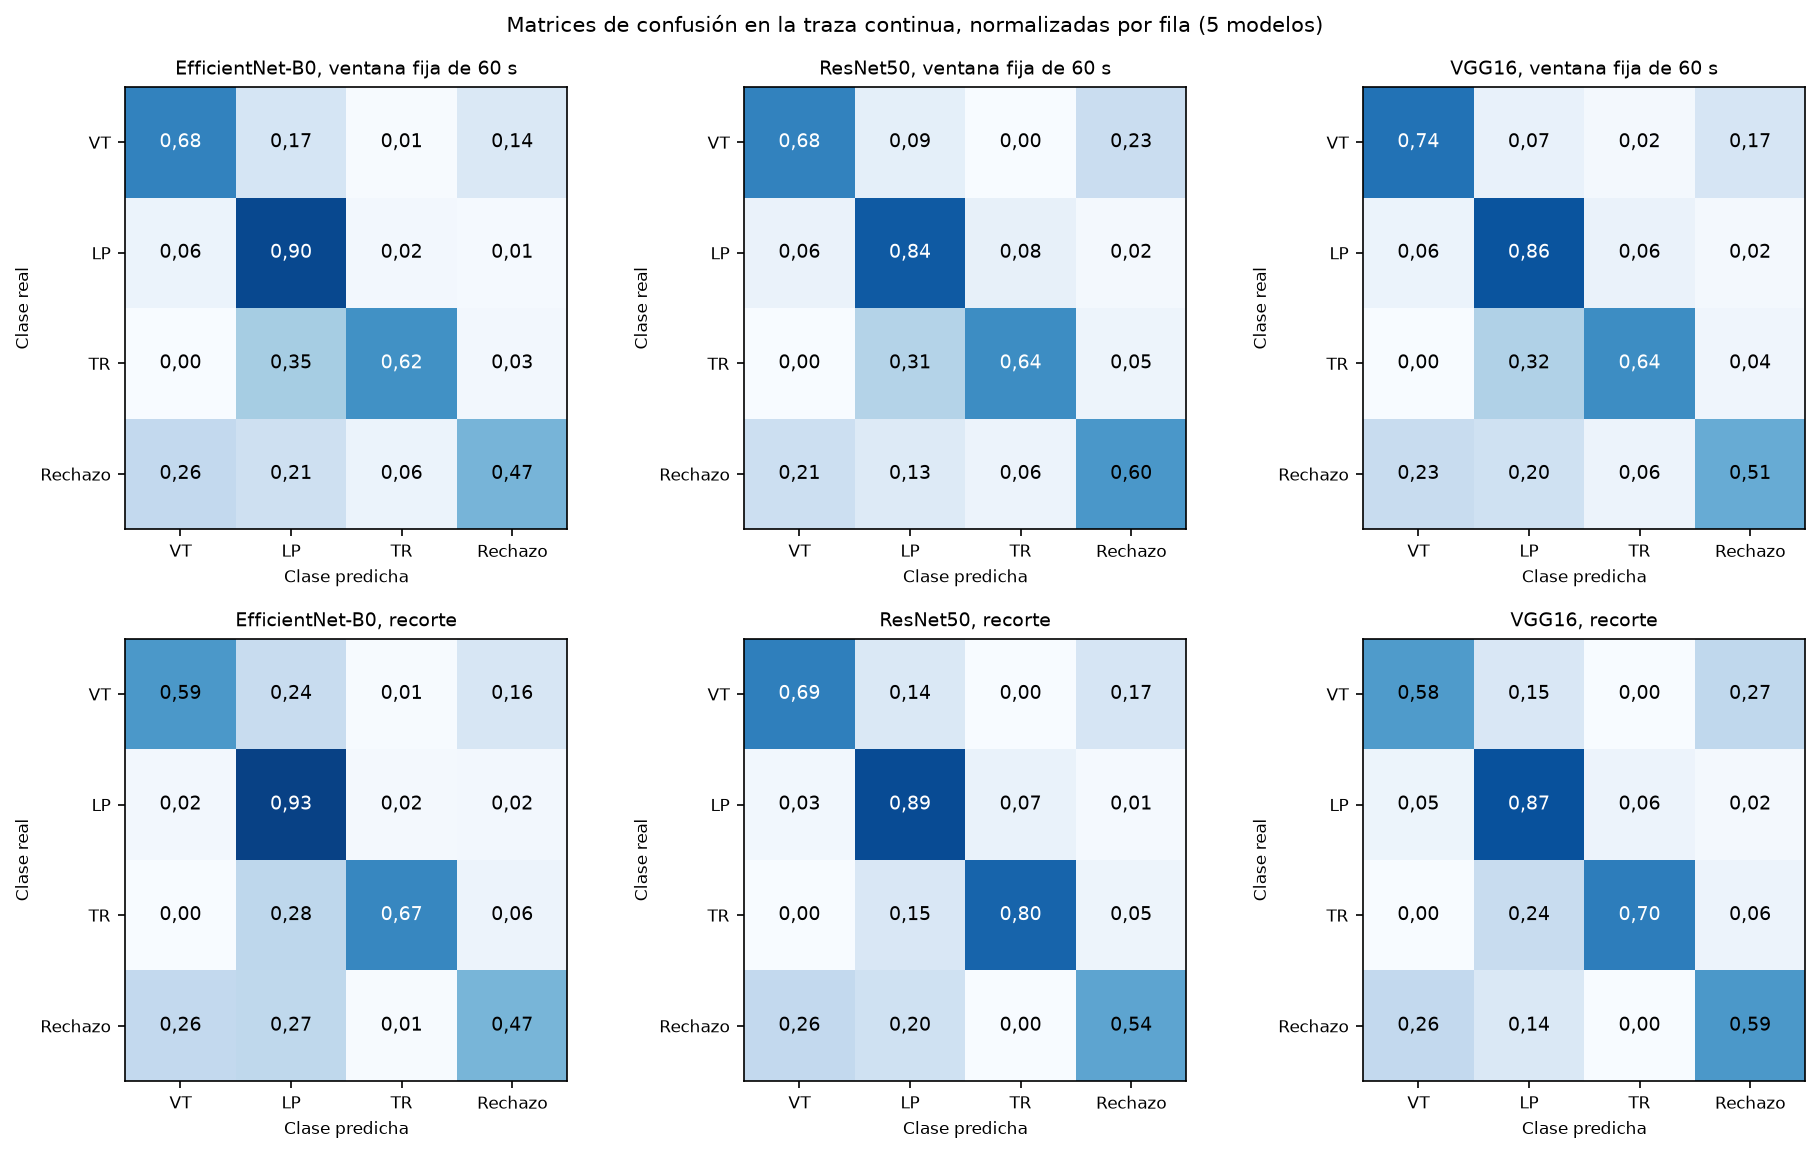
\includegraphics[width=\textwidth]{images/matrices_traza.png}
\caption{Matrices de confusión en la traza continua, normalizadas por fila
(suma de los cinco modelos de cada red). Arriba, con la ventana fija de
60\,s; abajo, con el recorte.}
\label{fig:res-matrices-traza}
\end{figure}

Los 855 recortes sin caja son 87,8 por hora de registro. El clasificador manda
a la clase de rechazo solo una parte de ellos: los que llama volcánicos son
entre 60,0 y 67,9 por hora con el recorte, según la red. Entre los cinco
modelos de una misma red esta cifra varía mucho; en ResNet50 va de 31,3 a 74,6
por hora.

\subsection{Tiempo de procesamiento}
\label{subsec:res-tiempo}

El Cuadro~\ref{tab:res-tiempo} da el tiempo de cada etapa sobre las 9,74 horas
de la traza, medido en el procesador del computador de trabajo, sin tarjeta
gráfica. La clasificación se da por modelo; en la evaluación se corrieron los
cinco modelos de cada red.

\needspace{9\baselineskip}
{\small
\begin{longtable}{lrr}
\caption{Tiempo de cada etapa sobre las 9,74 horas de la traza continua
(1.155 recortes).}\label{tab:res-tiempo}\\
\cabecera{\textbf{Etapa} & \textbf{Tiempo total (s)} & \textbf{Por recorte (ms)}}{3}
Detección con PhaseNet & 10,3 & --- \\
Recorte por energía & 0,3 & --- \\
Espectrogramas e imágenes & 13,1 & 11 \\
Clasificación con EfficientNet-B0 & 23,5 & 20,4 \\
Clasificación con ResNet50 & 52,1 & 45,1 \\
Clasificación con VGG16 & 78,1 & 67,6 \\
\end{longtable}
}

Con un modelo de EfficientNet-B0, la cadena completa procesa las 9,74 horas
en 47,2\,s, unas 740 veces más rápido que el tiempo real. Con ResNet50 toma
75,8\,s (unas 460 veces) y con VGG16, 101,8\,s (unas 340 veces). La red es la
etapa más lenta en las tres, y EfficientNet-B0, la red liviana, clasifica más
de tres veces más rápido que VGG16.

% =====================================================================
\section{Comprobaciones de la diferencia entre test y la traza}
\label{sec:res-comprobaciones}

El clasificador acierta menos en la traza continua que en test. Para acotar
por qué, se hicieron cuatro comprobaciones.

La primera es que la traza no se haya usado para entrenar. Ninguna de las
6.285 ventanas etiquetadas de origen, de las que salen las 5.669 con las tres
componentes completas, comparte tiempo con los tres tramos de la traza. La
traza no participó en el entrenamiento ni en la elección de la configuración
del clasificador.

La segunda es si la diferencia puede deberse al azar, porque en la traza hay
pocos recortes por clase. El Cuadro~\ref{tab:res-wilson} da, para cada red, la
sensibilidad de clasificación en la traza con su intervalo de confianza del
95\,\% (el promedio de los intervalos de los cinco modelos) y, al lado, el
promedio de test.

\needspace{9\baselineskip}
{\small
\setlength{\tabcolsep}{3pt}
\begin{longtable}{llrrlrl}
\caption{Sensibilidad de clasificación con el recorte en la traza, con su
intervalo de confianza del 95\,\%, y en test.}\label{tab:res-wilson}\\
\cabecera{\textbf{Red} & \textbf{Clase} & \textbf{Recortes} & \textbf{Traza} & \textbf{Intervalo} & \textbf{Test} & \textbf{¿Test dentro?}}{7}
EfficientNet-B0 & VT & 35 & 0,594 & [0,431; 0,739] & 0,893 & No \\
 & LP & 50 & 0,932 & [0,830; 0,972] & 0,869 & Sí \\
 & TR & 24 & 0,667 & [0,469; 0,818] & 0,764 & Sí \\
 & Rechazo & 40 & 0,465 & [0,322; 0,614] & 0,853 & No \\
\midrule
ResNet50 & VT & 35 & 0,691 & [0,528; 0,817] & 0,910 & No \\
 & LP & 50 & 0,892 & [0,778; 0,950] & 0,812 & Sí \\
 & TR & 24 & 0,800 & [0,606; 0,911] & 0,831 & Sí \\
 & Rechazo & 40 & 0,540 & [0,395; 0,678] & 0,857 & No \\
\midrule
VGG16 & VT & 35 & 0,583 & [0,421; 0,728] & 0,889 & No \\
 & LP & 50 & 0,872 & [0,753; 0,938] & 0,834 & Sí \\
 & TR & 24 & 0,700 & [0,501; 0,844] & 0,811 & Sí \\
 & Rechazo & 40 & 0,595 & [0,443; 0,731] & 0,904 & No \\
\end{longtable}
}

En VT y en el rechazo, el valor de test queda fuera del intervalo de la traza
en las tres redes: esa caída no se explica por el tamaño de la muestra. En LP y
TR el valor de test queda dentro del intervalo, así que con estos datos no se
puede decir que esas clases rindan distinto. Con la ventana fija de 60\,s pasa
lo mismo.

La tercera es si los recortes de la traza están peor delimitados que los de
test. No lo están: la mediana del IoU de los recortes con etiqueta de clase es
0,64 en test y 0,63 en la traza, y la parte con IoU de 0,5 o más es 0,75 y
0,71.

La cuarta mira, dentro de test, cómo cambia la sensibilidad según la posición
y la calidad del recorte. Las ventanas etiquetadas traen, además de la caja
principal al centro, cajas extra descentradas. El
Cuadro~\ref{tab:res-principal} compara las dos, y el
Cuadro~\ref{tab:res-iou-test} separa por IoU del recorte.

\needspace{9\baselineskip}
{\small
\setlength{\tabcolsep}{4pt}
\begin{longtable}{llrrrr}
\caption{Test con el recorte: sensibilidad por clase (promedio de los cinco
modelos) según el tipo de caja.}\label{tab:res-principal}\\
\cabecera{\textbf{Red} & \textbf{Caja} & \textbf{VT} & \textbf{LP} & \textbf{TR} & \textbf{Rechazo}}{6}
EfficientNet-B0 & Principal & 0,899 & 0,885 & 0,852 & 0,869 \\
 & Extra & 0,856 & 0,857 & 0,498 & 0,737 \\
ResNet50 & Principal & 0,919 & 0,853 & 0,914 & 0,869 \\
 & Extra & 0,847 & 0,783 & 0,584 & 0,774 \\
VGG16 & Principal & 0,896 & 0,867 & 0,887 & 0,913 \\
 & Extra & 0,842 & 0,811 & 0,584 & 0,837 \\
\midrule
Recortes & Principal & 293 & 281 & 183 & 282 \\
 & Extra & 43 & 395 & 61 & 38 \\
\end{longtable}
}

\needspace{9\baselineskip}
{\small
\setlength{\tabcolsep}{4pt}
\begin{longtable}{llrrrr}
\caption{Test con el recorte: sensibilidad por clase (promedio de los cinco
modelos) según el IoU del recorte con su caja.}\label{tab:res-iou-test}\\
\cabecera{\textbf{Red} & \textbf{IoU} & \textbf{VT} & \textbf{LP} & \textbf{TR} & \textbf{Rechazo}}{6}
EfficientNet-B0 & 0,3 a 0,5 & 0,919 & 0,886 & 0,590 & 0,791 \\
 & 0,5 a 0,7 & 0,936 & 0,880 & 0,833 & 0,876 \\
 & 0,7 o más & 0,831 & 0,852 & 0,918 & 0,881 \\
ResNet50 & 0,3 a 0,5 & 0,947 & 0,830 & 0,709 & 0,804 \\
 & 0,5 a 0,7 & 0,944 & 0,819 & 0,890 & 0,879 \\
 & 0,7 o más & 0,848 & 0,799 & 0,930 & 0,879 \\
VGG16 & 0,3 a 0,5 & 0,933 & 0,830 & 0,664 & 0,857 \\
 & 0,5 a 0,7 & 0,920 & 0,849 & 0,887 & 0,920 \\
 & 0,7 o más & 0,829 & 0,823 & 0,928 & 0,926 \\
\midrule
Recortes & 0,3 a 0,5 & 72 & 126 & 97 & 91 \\
 & 0,5 a 0,7 & 140 & 250 & 67 & 140 \\
 & 0,7 o más & 124 & 300 & 80 & 89 \\
\end{longtable}
}

Las cajas extra se clasifican peor que las principales, sobre todo en TR
(entre 0,50 y 0,58 contra entre 0,85 y 0,91). Las cajas extra difieren
también en otras cosas, como ser eventos secundarios de su ventana, así que
esta comparación no aísla el efecto de que el evento esté descentrado. En la
traza, cada recorte se clasifica en una ventana centrada en él, como las cajas
principales. Por IoU, TR depende mucho del recorte: con IoU entre 0,3 y 0,5 se
acierta entre 0,59 y 0,71, y con 0,7 o más, entre 0,92 y 0,93. En LP la
sensibilidad casi no cambia con el IoU, y en VT baja algo con IoU de 0,7 o
más.

Quedan sin medir dos posibles causas de la caída en VT y en el rechazo: que el
catálogo de la traza y el de las ventanas etiquetadas asignen las clases con
criterios distintos, y que los tramos de la traza correspondan a épocas o
condiciones del volcán distintas de las del entrenamiento. Se discuten en el
Capítulo~\ref{cap:discusion}.

\chapter{Discusión y análisis de resultados}
\label{cap:discusion}

Este capítulo interpreta los resultados del Capítulo~\ref{cap:resultados},
los compara con trabajos anteriores sobre el mismo problema y declara sus
limitaciones. Se separa lo que se midió de lo que se interpreta: cuando una
explicación no se comprobó con datos, se dice.

% =====================================================================
\section{Detección}
\label{sec:disc-deteccion}

En un sistema de vigilancia, perder un evento es más grave que dar una falsa
alarma. El evento perdido ya no llega al clasificador, mientras que la falsa
alarma todavía puede terminar en la clase de rechazo. Por eso la meta se puso
en la sensibilidad. Con esa meta, la comparación favorece a PhaseNet: es el
único detector que llega a 0,95 de los volcánicos (119 de 125) y mantiene la
meta cuando se mide en tramos que no se usaron para elegir sus umbrales (0,960
en la rotación de tramos). EQTransformer, con su curva de detección, queda
cerca (0,936) y con menos falsas alarmas (52,7 por hora contra 69,0), pero no
llega, y los intervalos que entrega son demasiado cortos para delimitar los
eventos: solo 31 de 125 quedan bien recortados. STA/LTA es el que da menos
falsas alarmas, pero detecta 0,848 de los volcánicos y su recorte pierde casi
todos los TR.

La ventaja de PhaseNet viene casi entera de la onda S. Con el umbral de la
onda P en 0,40 y el de la S en 0,05, la S detecta 47 volcánicos que la P no
ve, y la P solo 3 que la S no ve. Una explicación posible es que en los LP y
los TR la energía llega de forma gradual, sin el golpe nítido de una onda P de
sismo tectónico, que es con lo que se entrenó la red; no se comprobó. El costo
de depender de la S es doble: PhaseNet necesita un umbral muy bajo, con 69
falsas alarmas por hora, y cuando solo avisa la S el recorte empieza tarde.

La sensibilidad de 0,952 pasa la meta, pero su intervalo de confianza va de
0,899 a 0,978: con 125 eventos no se puede asegurar que el detector supere
0,95 con otro grupo de eventos parecido. Las ventanas de test, que no se
usaron para elegir ningún parámetro, dan una medición independiente: ahí
PhaseNet detecta 845 de 869 eventos principales (0,972), con un intervalo, de
0,959 a 0,981, que queda entero sobre la meta. Las dos mediciones son
coherentes entre sí.

La forma de contar pesa tanto como el detector. Con un aviso a 5\,s del
inicio, PhaseNet detectaba 0,904 de los volcánicos con umbral 0,10, y con
10\,s, 0,968; la diferencia eran solo TR, cuyo aviso cae dentro del evento y
lejos de su inicio. Contar por intersección evita elegir esa tolerancia, que
no viene de ninguna librería, y trata igual a los tres detectores. Su
contrapartida es que cuenta como detectado un evento que el intervalo apenas
toca; por eso la detección se informa siempre junto con el IoU del recorte.

La rotación de tramos mostró que, con más parámetros para elegir, la elección
se ajusta a los eventos con que se hace. En PhaseNet, cambiar también las
ventanas bajaba las falsas alarmas de 69,0 a 48,1 por hora con la traza
completa, pero en tramos nuevos la sensibilidad caía a 0,928. Con 125 eventos
repartidos de forma desigual entre tres tramos la prueba es limitada, pero es
la única forma disponible con estos datos de separar la elección de la
evaluación.

Las falsas alarmas son muchas: unas 69 por hora, casi seis por cada volcánico
detectado. Es un nivel parecido al que informa \textcite{soto2016llaima} para
el detector del volcán Llaima con una estación, cuya FDR era de 0,77 antes de
agregar una etapa que descartaba falsas detecciones y la bajaba a 0,42. En
este trabajo esa tarea queda en manos de la clase de rechazo, que no se
entrenó con falsas alarmas (Sección~\ref{sec:disc-clasificador}).

% =====================================================================
\section{Recorte y espectrogramas}
\label{sec:disc-recorte}

El recorte por energía cumple su papel con VT y LP: en la traza quedan bien
recortados 35 de 36 VT y 49 de 52 LP, y en test, 293 de 300 VT y 281 de 288
LP. Su punto débil es el tremor, que queda bien recortado en 0,65 de los casos
tanto en la traza (24 de 37) como en test (183 de 281). Las mediciones
señalan tres causas. La primera es que el aviso de los TR viene casi siempre
de la onda S y llega en mediana 12,9\,s después del inicio, así que el recorte
empieza tarde. La segunda es que PhaseNet da varios avisos dentro de un mismo
tremor, y el corte en el aviso siguiente lo parte. La tercera es que algunos
TR casi no sobresalen del ruido en FRE y el criterio de energía los termina
antes de tiempo. El corte en el aviso siguiente es un compromiso: suma 12 LP
bien recortados y resta 3 TR.

La duración variable de los eventos se resolvió estirando las columnas del
recorte hasta el ancho de entrada de la red. La ventana fija de 60\,s rinde
casi lo mismo en test (F1 macro de 0,831 a 0,835, contra 0,834 a 0,843 con el
recorte) y en la traza (0,708 a 0,720, contra 0,717 a 0,770). En el promedio,
entonces, el recorte variable no da una ventaja medible. La diferencia
aparece en el tremor cuando el recorte es bueno: con el inicio y el fin del
catálogo, TR se reconoce entre 0,784 y 0,859 con el recorte y entre 0,535 y
0,643 con la ventana fija. Cuando el evento está bien delimitado, conocer su
duración ayuda a reconocer el tremor; el problema de esa clase no está en la
imagen de duración variable, sino en el recorte automático.

Los errores de delimitación se trataron en dos lugares: al etiquetar, aceptando
recortes con IoU de 0,3 o más con su evento, y al entrenar, con la deformación
elástica en el eje del tiempo. Las mediciones por IoU en test muestran que VT
y LP toleran bien esos errores: la sensibilidad de LP casi no cambia con el IoU
y la de VT es incluso algo mayor con IoU bajo que con IoU de 0,7 o más. TR no
los tolera: con IoU entre 0,3 y 0,5 se acierta entre 0,59 y 0,71, y con 0,7 o
más, sobre 0,92.

% =====================================================================
\section{Clasificador}
\label{sec:disc-clasificador}

Las tres redes rinden lo mismo dentro de la variación entre folds: en test, el
F1 macro de VT, LP y TR va de 0,834 a 0,843, con desviaciones de 0,008 a 0,012
y diferencias entre redes menores que la distancia entre el mejor y el peor
modelo de una misma red. Esto le da sentido a la red liviana. EfficientNet-B0,
con unos 5 millones de parámetros en su versión para ImageNet, contra unos 138
millones de VGG16, clasifica más de tres veces más rápido sin perder
desempeño. Con estos resultados no hay razón de desempeño para preferir una
red más grande.

La búsqueda de la configuración, el aumento de datos y la parada temprana
subieron el F1 macro de validación en 0,02 a 0,03. Es una mejora del mismo
orden que la variación entre folds, así que su efecto es modesto. La búsqueda
se hizo con un solo fold y 20 pruebas por red; una búsqueda más amplia podría
encontrar algo mejor, pero no se repitió después de ver test ni la traza,
porque eso sería elegir con los datos de evaluación.

La confusión principal es TR con LP: entre el 13 y el 21\,\% de los TR de test
se clasifican como LP. Las dos clases concentran su energía en frecuencias
bajas, y el tremor se distingue sobre todo por durar más. Las mediciones por
IoU son coherentes con eso: un TR mal recortado, con IoU entre 0,3 y 0,5, se
acierta mucho menos que uno bien recortado.

El punto más débil del clasificador para operar sobre registro continuo son
los recortes sin caja, es decir, los que no tocan ningún evento del catálogo.
Por decisión de método no se usaron para entrenar, porque no se sabe qué son,
y el clasificador manda a la clase de rechazo solo entre un cuarto y un tercio
de ellos. En la traza eso deja entre 60 y 68 recortes por hora llamados
volcánicos sin un evento del catálogo detrás. Una parte podría ser eventos
reales que el catálogo no registró; no se revisó.

% =====================================================================
\section{Sistema completo: dónde se pierde el desempeño}
\label{sec:disc-sistema}

Las mediciones permiten repartir la pérdida del sistema completo. En la traza,
la detección y el recorte dejan bien delimitados 109 de los 125 volcánicos,
lo que pone un techo de 0,872 a la sensibilidad completa; la clasificación la
baja a entre 0,646 y 0,704. La comparación con el recorte de referencia
muestra que lo que cuesta el recorte se concentra en TR: con el inicio y el
fin del catálogo, TR se acierta entre 0,784 y 0,859, y con el sistema, entre
0,432 y 0,519. En VT y LP el recorte automático no cuesta nada medible, y
cuando calza con su evento, clasificar con él rinde igual que con el de
referencia: las diferencias volcánicas van de $-$0,007 a +0,044, con
intervalos que incluyen el cero. Esto responde la pregunta que dio origen al
OE4. Para un clasificador entrenado con recortes automáticos, pasar del recorte
de referencia al automático no degrada la clasificación cuando el recorte
calza; la pérdida viene de los eventos, casi todos TR, que el detector y el
recorte no alcanzan a delimitar.

La otra pérdida, la de VT y la de la clase de rechazo, no viene del recorte.
Con el recorte del catálogo, VT se acierta entre 0,567 y 0,589, igual que con
el automático y muy por debajo de test (0,889 a 0,910). Las comprobaciones
descartaron también que la traza se haya usado para entrenar y que sus
recortes estén peor delimitados que los de test. En la traza, los VT se
confunden con LP y con rechazo, y una cuarta parte del rechazo va a VT. Quedan
dos explicaciones posibles, ninguna medida. Una es que el catálogo de la traza
y el de las ventanas etiquetadas asignen VT, AV e IC con criterios distintos.
La otra es que los tres tramos de la traza correspondan a condiciones del
volcán o del ruido que el entrenamiento no cubre bien, aunque las ventanas de
entrenamiento abarcan de 2014 a 2020 y los tramos son de 2017, 2018 y 2020.
Con 35 VT y 40 eventos de rechazo no se puede separar una de otra; una
revisión de esos eventos por un analista sería la forma directa de hacerlo.

En tiempo, la cadena completa procesa las 9,74 horas de la traza entre 47 y
102\,s según la red, en el procesador de un computador personal y sin tarjeta
gráfica: entre 340 y 740 veces más rápido que el tiempo real. El tiempo no es
una restricción para operar en línea, y la red puede elegirse por desempeño y
no por costo.

% =====================================================================
\section{Comparación con trabajos anteriores}
\label{sec:disc-comparacion}

Los trabajos más cercanos usan el mismo volcán y el mismo conjunto publicado.
\textcite{espinosacurilem2026segmentacion} segmentan con una UNet ventanas de
81,92\,s armadas con la componente vertical de hasta ocho estaciones, y
obtienen en su conjunto de prueba un F1 macro de 0,91 sobre cinco clases (VT
0,92, LP 0,88, TR 0,93, AV 0,90 e IC 0,93) y un IoU medio de 0,88.
\textcite{espinosacurilem2025ood} combinan un VGG16 con un detector de señales
desconocidas y reportan un 84,3\,\% de acierto en las clases volcánicas y un
93,5\,\% en reconocer las no volcánicas. En este trabajo, el F1 macro de VT,
LP y TR en test va de 0,834 a 0,843, con F1 por clase de 0,84 a 0,85 en VT, de
0,86 a 0,87 en LP y de 0,79 a 0,82 en TR.

Las cifras no se pueden comparar directamente, y la diferencia no debe leerse
como una diferencia entre métodos, porque cambian tres condiciones. Aquí se
usa una sola estación y allá hasta ocho, y combinar estaciones mejora el
acierto: \textcite{curilem2016estaciones} midieron una mejora media de 9\,\% en
el volcán Llaima. Aquí cada evento llega recortado por el detector, con su
error de inicio y fin, y allá viene aislado en su ventana. Y los conjuntos de
prueba difieren en composición y en balance de clases. Aun así, la diferencia
mayor está en TR (0,93 contra 0,79 a 0,82), que es justamente la clase que el
recorte automático delimita peor.

El trabajo de \textcite{soto2016llaima}, sobre el volcán Llaima y con una
estación, enfrentó la misma pregunta con un clasificador de máquinas de
vectores de soporte. Entrenado con recortes del detector, rindió 85,05\,\% de
sensibilidad media con esos recortes y 83,69\,\% con los de analistas, y
concluyó que conviene entrenar con los recortes del detector. Aquí el
clasificador también se entrenó con recortes automáticos, y la comparación
pareada en la traza lleva a la misma conclusión con otra técnica y otro
volcán. En operación continua, ese trabajo midió 77,30\,\% de sensibilidad
media de clasificación y 66,04\,\% para el sistema completo, y reporta que,
con una sola estación, ni los analistas superaban el 70\,\% de acierto. Aquí la
sensibilidad completa volcánica va de 0,646 a 0,704. Las medidas no son
iguales, porque allá se multiplica la sensibilidad media de detección por la
de clasificación y aquí se exige que cada evento se detecte, se recorte y se
clasifique bien a la vez; pero en los dos casos el sistema completo queda
claramente por debajo de lo que cada etapa logra por separado.

% =====================================================================
\section{Cumplimiento de los objetivos}
\label{sec:disc-objetivos}

El Cuadro~\ref{tab:disc-objetivos} resume, para cada objetivo específico, lo
que se pidió y lo que se obtuvo. El cumplimiento de cada requerimiento, el
resultado de los criterios de aceptación y el estado final de cada tarea del
backlog están en los Anexos~\ref{sec:anexo-cumplimiento},
\ref{sec:anexo-aceptacion} y~\ref{sec:anexo-estado-backlog}.

{\small
\setlength{\tabcolsep}{4pt}
\begin{longtable}{>{\raggedright\arraybackslash}p{1.0cm}>{\raggedright\arraybackslash}p{4.2cm}>{\raggedright\arraybackslash}p{7.0cm}}
\caption{Cumplimiento de los objetivos específicos.}\label{tab:disc-objetivos}\\
\cabecera{\textbf{Obj.} & \textbf{Qué pide} & \textbf{Qué se obtuvo}}{3}
OE1 & Evaluar STA/LTA, EQTransformer y PhaseNet sobre registro continuo
etiquetado: sensibilidad, falsas alarmas y calidad del recorte (IoU) &
Cumplido. Los tres se evaluaron con la misma forma de contar, con barrido de
sus parámetros y rotación de tramos. PhaseNet es el único que llega a la meta:
0,952 [0,899; 0,978] con 69,0 falsas alarmas por hora; su recorte por energía
deja bien delimitados 0,864 de los volcánicos
(Sección~\ref{sec:res-detectores} y Sección~\ref{sec:res-recorte}). \\
\addlinespace
OE2 & Generar espectrogramas desde los eventos detectados, considerando su
duración variable, los errores de delimitación y el solapamiento &
Cumplido. El recorte se estira a la entrada de la red (duración variable), se
etiqueta con IoU de 0,3 o más y se entrena con deformación elástica (errores
de delimitación), y se corta en el aviso siguiente (solapamiento). TR es la
clase peor recortada: 0,65 en la traza y en test
(Sección~\ref{sec:recorte-espectrogramas} y
Sección~\ref{sec:res-deteccion-test}). \\
\addlinespace
OE3 & Ajustar por transferencia una CNN que clasifique en VT, LP, TR y
rechazo, con protocolo reproducible &
Cumplido con tres redes (VGG16, ResNet50 y EfficientNet-B0), búsqueda de la
configuración y validación cruzada de cinco folds. F1 macro de VT, LP y TR en
test de 0,834 a 0,843. Los datos, las particiones y la semilla quedan fijos;
no se comprobó repitiendo una corrida que dé exactamente lo mismo
(Sección~\ref{sec:res-clasificador}). \\
\addlinespace
OE4 & Evaluar el sistema integrado sobre registro continuo: recorte de
referencia contra automático, por clase y con tiempo de procesamiento &
Cumplido. Sensibilidad completa volcánica de 0,646 a 0,704; frente al recorte
de referencia, el sistema pierde entre 0,056 y 0,098, casi todo en TR, y sin
pérdida cuando el recorte calza. La cadena procesa 9,74 horas en 47 a 102\,s
en CPU (Sección~\ref{sec:res-sistema}). \\
\end{longtable}
}

% =====================================================================
\section{Limitaciones}
\label{sec:disc-limitaciones}

Todo el sistema usa una sola estación, FRE. Los trabajos con varias
estaciones rinden más, y la asociación entre estaciones es la forma habitual de
descartar falsas alarmas, pero queda fuera del alcance de este trabajo.

La traza continua tiene 125 eventos volcánicos, y algunas clases quedan con
pocos recortes (24 TR bien recortados, 35 VT). Los intervalos de confianza
son anchos y varias diferencias no se pueden distinguir del azar. Además, los
umbrales del detector se eligieron con la misma traza con que se evalúa; la
rotación de tramos y las ventanas de test atenúan ese problema, pero no lo
eliminan.

Los detectores se usaron con los pesos publicados, entrenados con sismos
tectónicos, sin ajustarlos con datos volcánicos. El recorte por energía, el
umbral de IoU de 0,3 y los límites del aumento de datos (desplazamiento del
rango de colores de hasta 5\,dB, ancho de 50 a 70\,dB y deformación solo en el
tiempo) son decisiones propias de este trabajo, explicadas en el
Capítulo~\ref{cap:diseno}, y otras elecciones podrían cambiar los resultados.

Los recortes sin caja no se usaron para entrenar, y el clasificador llama
volcánicos a la mayoría de ellos. El catálogo se tomó como la verdad, sin
medir cuánto concuerdan distintos analistas al etiquetar, y esa es una de las
posibles explicaciones de la caída de VT en la traza que quedó sin comprobar.
La búsqueda de la configuración usó un solo fold y 20 pruebas por red.
Finalmente, la evaluación es fuera de línea, sobre registro guardado; no se
probó el sistema recibiendo señal en tiempo real.

\chapter{Conclusiones}
\label{cap:conclusiones}

Este trabajo desarrolló un sistema que identifica eventos sismo-volcánicos del
Complejo Volcánico Nevados de Chillán en registro continuo: detecta los
eventos con PhaseNet en la estación FRE, recorta cada uno según su energía,
genera su espectrograma y lo clasifica en VT, LP, TR o rechazo con una red
convolucional ajustada por transferencia de aprendizaje. El problema planteado
en el Capítulo~\ref{cap:introduccion} señalaba que faltaban tres cosas: evidencia
local de qué detector conviene usar, un recorte que se ajuste a la duración
real de los eventos y una medición de cuánto desempeño pierde el clasificador
al pasar de recortes de referencia a recortes automáticos. Las tres quedaron
medidas.

\section{Conclusiones por objetivo}

Sobre la detección (OE1), PhaseNet es el único de los tres detectores que
llega a la meta de 0,95 de sensibilidad volcánica sobre la traza continua
(0,952), la mantiene en tramos que no se usaron para elegir sus umbrales y la
supera en las ventanas de test (0,972). Lo logra gracias a la onda S y a un
umbral bajo, con un costo de unas 69 falsas alarmas por hora. EQTransformer
queda cerca con menos falsas alarmas, pero sus intervalos son demasiado cortos
para delimitar los eventos, y STA/LTA pierde casi todos los tremores al
recortar. También se mostró que la forma de contar una detección cambia el
resultado tanto como el detector; contar por intersección evita depender de
una tolerancia elegida a mano.

Sobre el recorte y los espectrogramas (OE2), el recorte por energía con corte
en el aviso siguiente delimita bien 0,864 de los volcánicos de la traza y casi
todos los VT y LP de test. El tremor es su límite: solo 0,65 de los TR quedan
bien recortados, porque el aviso llega tarde, porque PhaseNet avisa varias
veces dentro de un mismo tremor y porque algunos casi no sobresalen del ruido.
Con un buen recorte, la duración variable ayuda a reconocer el tremor; en
promedio, el recorte y la ventana fija de 60\,s rinden lo mismo.

Sobre el clasificador (OE3), VGG16, ResNet50 y EfficientNet-B0 alcanzan en
test un F1 macro de VT, LP y TR de 0,834 a 0,843, sin diferencias entre ellas
mayores que la variación entre folds. La búsqueda de la configuración y el
aumento de datos aportaron entre 0,02 y 0,03. La red liviana, EfficientNet-B0,
rinde igual que las grandes y clasifica más de tres veces más rápido que
VGG16. La confusión principal es entre TR y LP, y el clasificador manda a la
clase de rechazo solo una parte de las falsas alarmas del detector.

Sobre el sistema completo (OE4), en la traza continua el sistema detecta,
recorta y clasifica bien entre 0,646 y 0,704 de los volcánicos, y procesa las
9,74 horas en menos de dos minutos en un computador personal. Frente al
recorte de referencia, el sistema pierde entre 0,056 y 0,098 de sensibilidad
volcánica, casi todo en TR; cuando el recorte automático calza con su evento,
clasificar con él rinde lo mismo que con el de referencia. La pérdida en VT y
en la clase de rechazo frente a test no viene del recorte, y queda sin
explicar con los datos disponibles.

En conjunto, el sistema cumple el objetivo general. Su desempeño en registro
continuo queda por debajo del que logra cada etapa por separado, como ocurrió
en trabajos anteriores con una sola estación, y las mediciones dicen dónde se
pierde: en el recorte de los tremores, en la clasificación de VT y en las
falsas alarmas que el clasificador no rechaza.

\section{Recomendaciones y trabajo futuro}

Las recomendaciones salen de lo que los resultados mostraron como más débil.

Entrenar la clase de rechazo también con recortes que no corresponden a ningún
evento, o agregar una etapa que descarte falsas detecciones antes del
clasificador, como la que usó \textcite{soto2016llaima}. Es la vía más directa
para bajar las falsas alarmas que hoy llegan como volcánicas, y debe medirse
cuánto cuesta en sensibilidad.

Mejorar el recorte de los tremores sin usar información del catálogo, por
ejemplo juntando los avisos que caen dentro de un mismo tremor o usando la
curva de detección de EQTransformer para fijar el fin del evento. Cualquier
cambio debe compararse con el recorte actual usando el mismo IoU y la misma
traza.

Incorporar más estaciones. La asociación de avisos entre estaciones es la
forma habitual de descartar falsas alarmas, y combinar estaciones mejora la
clasificación en otros volcanes \parencite{curilem2016estaciones}.

Revisar con un analista los VT y los eventos de rechazo de la traza que el
clasificador confunde, para saber si la caída frente a test se debe a cómo se
etiquetaron o a la señal misma.

Ajustar PhaseNet y EQTransformer con datos volcánicos, para que reconozcan la
llegada gradual de los LP y los TR sin depender de umbrales tan bajos.

Evaluar el sistema con más horas de registro continuo y más eventos, para
estrechar los intervalos de confianza, y probarlo recibiendo señal en tiempo
real.


\printbibliography
\appendix
\chapter{Anexos}

\section{Glosario de términos y siglas}
\label{sec:anexo-glosario}

Este glosario explica, en palabras simples, los términos y las siglas que
aparecen en el documento, para que pueda leerlo alguien sin formación en
volcanes, en sismología ni en programación. Cada término se explica también la
primera vez que aparece en el texto.

{\small
\setlength{\tabcolsep}{4pt}
\begin{longtable}{>{\raggedright\arraybackslash}p{3.4cm}>{\raggedright\arraybackslash}p{9.4cm}}
\caption{Glosario de términos y siglas.}\label{tab:glosario}\\
\cabecera{\textbf{Término} & \textbf{Significado}}{2}
AdamW & Optimizador que ajusta los pesos de la red según el promedio de sus
cambios recientes y que, además, los achica un poco en cada paso. Ver
\emph{optimizador}. \\
Aprendizaje profundo & Forma de aprendizaje automático que usa redes
neuronales con muchas capas. \\
Aumento de datos & Cambios al azar que se hacen a las imágenes de
entrenamiento en cada época, para que la red no memorice los ejemplos. Aquí se
cambia el rango de colores del espectrograma y se deforma levemente la imagen
en el eje del tiempo. \\
AV (avalancha) & Señal producida por el deslizamiento de rocas, nieve o hielo
por las laderas del volcán. No informa sobre el interior del volcán, así que va
a la clase de rechazo. \\
Aviso & Instante en que un detector indica que podría haber un evento. En
PhaseNet, cada aviso es también un intervalo: desde que la probabilidad de la
onda supera su umbral hasta que baja de la mitad de ese umbral. \\
\emph{Blinding} & Parámetro de SeisBench: cuántas muestras se descartan en cada
borde de la ventana que lee la red, porque cerca del borde la red ve la señal
hacia un solo lado. \\
\emph{Bootstrap} & Forma de estimar la incertidumbre de un resultado: se
sortean con reemplazo, muchas veces, grupos de datos del mismo tamaño que el
original, se repite el cálculo en cada uno y se mira cuánto cambia. \\
Caja & Inicio y fin de un evento marcados en el catálogo dentro de una ventana
etiquetada. La caja principal es la del evento que está al centro de la
ventana; las cajas extra son las de otros eventos que caen en ella. \\
Catálogo & Lista de eventos con su inicio, su fin y su clase, marcados por
analistas. Se usa como la verdad para evaluar. \\
Clase & Tipo de evento. Aquí, VT, LP y TR (volcánicos), y AV e IC (no
volcánicos). \\
Clase de rechazo & Salida del clasificador para lo que no es volcánico. Se
entrena con AV e IC. \\
Clasificador & Programa que, dada la imagen de un evento, decide a qué clase
pertenece. \\
CNN (red neuronal convolucional) & Red neuronal hecha para imágenes: aprende a
reconocer patrones simples, como bordes y texturas, y los combina en patrones
más complejos. \\
Componente & Dirección del movimiento del suelo que registra un sensor: Z
(vertical), N (norte-sur) y E (este-oeste). \\
CPU y GPU & La CPU es el procesador principal de un computador. La GPU es la
tarjeta gráfica, que hace muchas operaciones a la vez y acelera el
entrenamiento de redes neuronales. CUDA es el sistema de NVIDIA para usarla. \\
Decibel (dB) & Escala para expresar energía en la que cada 10\,dB equivalen a
multiplicar la energía por diez. Aquí, la energía de cada frecuencia en el
espectrograma. \\
Desviación estándar & Medida de cuánto se alejan los valores de su promedio. \\
Detector & Programa que recorre la señal continua y marca dónde parece haber
un evento. \\
\emph{Dropout} & Técnica que, durante el entrenamiento, apaga al azar una parte
de las neuronas, para que la red no dependa de unas pocas. \\
EfficientNet-B0 & Red convolucional liviana, diseñada para rendir bien con
pocos parámetros. \\
Entropía cruzada & Función de pérdida habitual en clasificación: mide qué tan
lejos está la probabilidad que da la red de la clase correcta. \emph{Con
pesos}, los errores en las clases con menos ejemplos cuentan más. \\
Envolvente & Curva que sigue la amplitud de la señal sin sus oscilaciones. El
recorte por energía la usa para decidir dónde termina un evento. \\
Época & Una pasada completa por todas las imágenes de entrenamiento. \\
EQTransformer & Red neuronal publicada para detectar sismos y marcar sus ondas
P y S. Además de las ondas, entrega una curva de detección con el inicio y el
fin del evento. \\
Espectrograma & Imagen que muestra cómo se reparte la energía de una señal
entre las frecuencias a lo largo del tiempo: el eje horizontal es el tiempo,
el vertical la frecuencia y el color la energía. \\
Estación sismológica & Lugar donde un sensor registra el movimiento del suelo.
FRE es la estación usada en este trabajo. \\
Evento & Señal sísmica que se distingue del ruido de fondo, con un inicio y un
fin. \\
F1 y F1 macro & El F1 combina en un número entre 0 y 1 la sensibilidad y la
precisión de una clase. El F1 macro es el promedio simple del F1 de varias
clases; aquí, de VT, LP y TR. \\
Falsa alarma & Detección que no corresponde a ningún evento del catálogo.
FP/h son las falsas alarmas por hora de registro. \\
FDR & Del inglés \emph{false discovery rate}: la parte de las detecciones que
son falsas alarmas. \\
Filtro pasa banda & Operación que deja pasar solo las frecuencias de un rango,
por ejemplo de 1 a 15\,Hz, y atenúa el resto. \\
Focal (pérdida) & Función de pérdida que da más peso a los ejemplos que la red
todavía clasifica mal. \\
Fold y validación cruzada & El conjunto de desarrollo se divide en cinco partes
o \emph{folds}. Se entrena cinco veces, cada vez validando con una parte
distinta y entrenando con las otras cuatro. \\
Frecuencia y Hz & Cuántas veces por segundo oscila una señal; se mide en
hercios (Hz). La frecuencia de muestreo es cuántos valores por segundo se
registran: aquí, 100\,Hz. \\
Fuera (etiqueta) & Recorte que toca un evento del catálogo pero con un IoU
menor que 0,3. No se usa para entrenar ni para medir la clasificación. \\
Función de pérdida & Número que mide cuánto se equivoca la red durante el
entrenamiento; entrenar consiste en reducirlo. \\
IC (\emph{ice-quake}) & Sismo producido por la fractura del hielo de los
glaciares del volcán. No es volcánico, así que va a la clase de rechazo. \\
ImageNet & Colección de más de un millón de fotografías etiquetadas, usada para
preentrenar redes de imágenes. \\
Intersección (detección por) & Criterio con que se cuenta una detección: un
evento está detectado si algún intervalo del detector comparte al menos un
instante con él. \\
Intervalo de confianza & Rango en que probablemente estaría un resultado si se
midiera con otro grupo de datos parecido. Aquí se usa el del 95\,\%. \\
IoU & Del inglés \emph{intersection over union}: el tiempo en común entre un
recorte y su evento, dividido por el tiempo total que cubren los dos. Vale 1
si coinciden y 0 si no se tocan. \\
Lote & Grupo de imágenes que la red procesa juntas antes de ajustar sus
pesos. \\
LP (largo período) & Evento volcánico de baja frecuencia, asociado al
movimiento de fluidos dentro del volcán; suele durar menos de un minuto. \\
Matriz de confusión & Tabla que cruza la clase real, en las filas, con la
clase que asignó el clasificador, en las columnas. Normalizada por fila, cada
fila muestra a dónde va cada clase. \\
Mediana & Valor que queda al medio cuando se ordenan los datos: la mitad queda
bajo él y la otra mitad sobre él. \\
Muestra & Cada valor registrado de la señal. A 100\,Hz hay 100 muestras por
segundo. \\
NVChVC & Complejo Volcánico Nevados de Chillán, en la Región de Ñuble,
Chile. \\
ObsPy & Librería de Python para procesar señales sísmicas. Aquí se usa para
STA/LTA y para los filtros. \\
OOD & Del inglés \emph{out of distribution}: una señal distinta de todo lo que
el clasificador vio al entrenar. \\
Onda P y onda S & Las dos primeras ondas que llegan de un sismo. La P llega
primero y empuja el suelo en la dirección en que viaja; la S llega después y
lo sacude de lado. \\
Optimizador & Método que ajusta los pesos de la red para reducir la función de
pérdida. AdamW y SGD son dos optimizadores. \\
Optuna y TPE & Optuna es una librería para buscar configuraciones; TPE es su
método por defecto, que propone nuevas pruebas cerca de las combinaciones que
mejor han rendido. \\
OVDAS & Observatorio Volcanológico de los Andes del Sur, del SERNAGEOMIN,
encargado de vigilar los volcanes de Chile. \\
\emph{Overlap} & Parámetro de SeisBench: cuántas muestras comparten dos
ventanas seguidas de la red. \\
Parada temprana & Detener el entrenamiento cuando la validación deja de mejorar
y quedarse con la mejor época. Aquí se detiene tras cinco épocas sin
mejora. \\
Parámetro & Valor que ajusta el comportamiento de un método, como un
umbral. \\
Percentil & El percentil 20 es el valor bajo el cual queda el 20\,\% de los
datos. \\
Pesos & Números internos de una red neuronal que se ajustan durante el
entrenamiento. \\
PhaseNet & Red neuronal publicada para marcar las ondas P y S de un sismo:
entrega, para cada instante, la probabilidad de que llegue cada onda. \\
Precisión & De lo que el sistema asigna a una clase, la parte que de verdad es
de esa clase. \\
Preentrenada (red) & Red que ya fue entrenada con otros datos y se usa como
punto de partida. \\
PyTorch y torchvision & PyTorch es una librería para construir y entrenar
redes neuronales; torchvision es su colección de redes de imágenes con pesos
preentrenados. \\
Recorte & Tramo de señal que el sistema asigna a un evento, con su inicio y su
fin. El recorte automático es el que fija el sistema; el recorte de referencia,
el que marca el catálogo. \\
Red neuronal & Modelo formado por capas de unidades simples conectadas, cuyos
pesos se ajustan a partir de ejemplos. \\
ResNet50 & Red convolucional de 50 capas con conexiones que saltan capas, lo
que facilita entrenar redes profundas. \\
Rotación de tramos & Elegir los parámetros de un detector con dos de los tres
tramos de la traza y medirlos en el tercero, repitiendo con las tres
combinaciones. \\
Ruido & Señal de fondo que no corresponde a un evento: viento, oleaje,
actividad humana o el propio sensor. \\
SeisBench & Librería de Python que reúne redes sísmicas preentrenadas, como
PhaseNet y EQTransformer, con una forma común de usarlas. \\
Semilla & Número que fija la secuencia de valores al azar de un programa, para
que una corrida se pueda repetir. \\
Sensibilidad & De los eventos de una clase, la parte que el sistema encuentra o
clasifica bien. La sensibilidad completa es la parte que el sistema detecta,
recorta y clasifica bien a la vez. \\
SERNAGEOMIN & Servicio Nacional de Geología y Minería de Chile. \\
SGD & Optimizador de descenso de gradiente estocástico: ajusta los pesos con
pasos en la dirección que más reduce la pérdida. Con \emph{momentum}, cada paso
conserva parte de la dirección del anterior. \\
Sin caja (etiqueta) & Recorte que no toca ningún evento del catálogo. No se usa
para entrenar, pero en operación el sistema lo recibe igual. \\
Sismo tectónico & Sismo producido por el movimiento de las placas de la corteza
terrestre, no por un volcán. PhaseNet y EQTransformer se entrenaron con
sismos de este tipo. \\
Slurm & Sistema que ordena en una cola los trabajos que se envían a un servidor
compartido. \\
\emph{Stacking} & Parámetro de SeisBench: cómo se juntan las predicciones de
ventanas que se solapan, por promedio o por máximo. \\
STA/LTA & Detector clásico que compara la energía media de una ventana corta
(STA) con la de una ventana larga (LTA) y avisa cuando la razón entre ambas
supera un umbral. \\
Tasa de aprendizaje & Tamaño de cada ajuste de los pesos durante el
entrenamiento. \\
Test & Conjunto de datos que se aparta al inicio y solo se usa para la
evaluación final. \\
TR (tremor) & Señal volcánica continua, de minutos a horas, asociada al
movimiento sostenido de fluidos dentro del volcán. \\
Transferencia de aprendizaje & Partir de una red ya entrenada para otra tarea
y ajustarla a la nueva. \\
Traza continua & Registro sísmico sin cortes de un periodo. Aquí, 10,18\,h en
tres tramos de fechas distintas. \\
Umbral & Valor que una medida debe superar para tomar una decisión, por
ejemplo para dar un aviso. \\
Validación & Datos que no se usan para entrenar y sirven para decidir cuándo
parar y qué configuración elegir. \\
Ventana & Tramo de señal de largo fijo. Una ventana etiquetada es un tramo de
300\,s con un evento al centro y las cajas de los eventos que contiene. \\
VGG16 & Red convolucional de 16 capas, de diseño simple y con muchos
parámetros. \\
VT (volcano-tectónico) & Evento volcánico producido por la ruptura de roca
debido a procesos volcánicos. Se parece a un sismo pequeño: es corto y tiene
frecuencias más altas que el LP. \\
\emph{Weight decay} & Penalización que achica los pesos de la red, para que no
se ajuste de más a los ejemplos de entrenamiento. \\
Wilson (intervalo de) & Método para calcular el intervalo de confianza de una
proporción que funciona bien con pocos datos. \\
Zenodo & Repositorio público de datos científicos donde está publicado el
conjunto de datos usado en este trabajo. \\
\end{longtable}
}

\section{Criterios SMART de los objetivos específicos}
\label{sec:anexo-smart}

Se desarrollan aquí los cinco criterios SMART de cada objetivo específico, en
su versión final. El criterio medible y la etapa de cierre están resumidos en
el Cuadro~\ref{tab:smart} de la Sección~\ref{subsec:smart}.

OE1. \emph{Específico}: compara tres detectores concretos, STA/LTA,
EQTransformer y PhaseNet, sobre un conjunto de datos delimitado.
\emph{Medible}: sensibilidad y falsas alarmas por hora, globales y por clase,
con intervalos de confianza del 95\,\% de Wilson; calidad del recorte por IoU
con varios umbrales; barrido de los parámetros de cada detector y costo de cada
nivel de sensibilidad en falsas alarmas. \emph{Alcanzable}: se ejecuta con
inferencia en CPU sobre modelos preentrenados, sin entrenar.
\emph{Relevante}: aborda los aspectos P1 y P2 del problema
(Cuadro~\ref{tab:trazabilidad}). \emph{Con plazo}: cerrado en la Etapa 2 y
repetido con las tres componentes de FRE en la Etapa 3.

OE2. \emph{Específico}: define un procedimiento de generación de
espectrogramas cuyo recorte sigue la duración de cada evento, y que tolera los
errores de delimitación y el solapamiento entre eventos. \emph{Medible}: IoU
del recorte por energía contra la ventana fija y contra los recortes propios de
los otros detectores, por clase; forma en que falla el recorte, al inicio o al
fin; sensibilidad del clasificador según el IoU del recorte.
\emph{Alcanzable}: opera sobre las salidas de OE1, sin hardware
especializado. \emph{Relevante}: aborda P3 y P1. \emph{Con plazo}: diseñado en
la Etapa 2 e implementado y medido en la Etapa 3.

OE3. \emph{Específico}: ajusta por transferencia de aprendizaje redes
convolucionales preentrenadas en ImageNet, con una salida de cuatro clases,
sobre los espectrogramas producidos por OE2. Se comparan VGG16, ResNet50 y
EfficientNet-B0. \emph{Medible}: F1 macro y sensibilidad por clase, con
promedio, mínimo, máximo y desviación de cinco folds; matrices de confusión de
cuatro clases; protocolo con particiones, semillas y configuración registradas.
\emph{Alcanzable}: el entrenamiento se hace en un servidor con GPU y la
inferencia en CPU; las 5.669 ventanas etiquetadas con las tres componentes de
FRE están disponibles. \emph{Relevante}: aborda P5. \emph{Con plazo}:
resultados preliminares en la Etapa 3 y completos en la Etapa 4.

OE4. \emph{Específico}: evalúa la cadena completa sobre el registro continuo,
comparando el desempeño del clasificador con recorte de referencia y con
recorte automático para los mismos eventos. \emph{Medible}: diferencia pareada
entre ambas condiciones con su intervalo de confianza por \emph{bootstrap};
resultados por clase; tiempo de procesamiento de la cadena completa en CPU.
\emph{Alcanzable}: reutiliza lo producido en OE1 a OE3 y solo requiere
inferencia en el equipo local. \emph{Relevante}: aborda P4. \emph{Con plazo}:
cerrado en la Etapa 4.


\section{Evidencia empírica de la evaluación inicial de detectores}
\label{sec:anexo-evidencia}

La evaluación inicial de detectores entregó nueve hallazgos que condicionaron
el diseño de los bloques posteriores. Todos corresponden a mediciones sobre la
traza continua de 10,18~horas con cinco estaciones y solo su componente
vertical, con un catálogo de 203 eventos utilizables, y son los que la
Sección~\ref{sec:evidencia} invoca como origen de los requerimientos
funcionales. Se conservan como registro de lo que motivó el diseño. La
evaluación final, con la estación FRE y sus tres componentes, está en el
Capítulo~\ref{cap:resultados}; con ella cambian E1 y E2, porque PhaseNet supera
a los otros dos detectores.

{\small
\begin{longtable}{>{\raggedright\arraybackslash}p{0.9cm}>{\raggedright\arraybackslash}p{5.3cm}>{\raggedright\arraybackslash}p{5.3cm}}
\caption{Hallazgos de la evaluación inicial de detectores y su implicación de diseño.}\label{tab:evidencia}\\
\toprule
\textbf{ID} & \textbf{Hallazgo medido} & \textbf{Implicación de diseño} \\
\midrule
\endfirsthead
\multicolumn{3}{l}{\itshape Cuadro \thetable{} (continuación)}\\
\toprule
\textbf{ID} & \textbf{Hallazgo medido} & \textbf{Implicación de diseño} \\
\midrule
\endhead
\midrule
\multicolumn{3}{r}{\itshape Continúa en la página siguiente}\\
\endfoot
\bottomrule
\endlastfoot
E1 & El recall global de los tres detectores es estadísticamente indistinguible:
0,542; 0,527 y 0,581, con intervalos de confianza del 95\,\% solapados &
El detector no puede seleccionarse por su recall global \\
\addlinespace
E2 & Por clase existen diferencias significativas de signo opuesto que se cancelan
al promediar: un detector aventaja en LP y TR, el otro en VT, AV e IC &
Toda métrica debe reportarse desagregada por clase \\
\addlinespace
E3 & En calidad de delimitación, STA/LTA supera a EQTransformer de forma robusta
frente al umbral de solapamiento: IoU de 0,563 contra 0,479 &
La variabilidad del recorte entre detectores es un hecho medido; el clasificador
debe absorberla \\
\addlinespace
E4 & PhaseNet no delimita eventos: entrega arribos, no intervalos &
Se requiere una regla explícita de expansión de arribo a intervalo \\
\addlinespace
E5 & La mediana de duración de TR es de 87,8~s y excede la ventana fija de
81,92~s; el rango observado va de 3,4~s a 240,8~s &
El recorte debe ser adaptativo: la ventana fija trunca la clase más extensa \\
\addlinespace
E6 & 73 de los 203 eventos del catálogo continuo, un 36\,\%, son de clases no
volcánicas, y los detectores las encuentran con buen desempeño &
El rechazo no puede ocurrir en la detección; debe resolverse en la clasificación \\
\addlinespace
E7 & De 106 falsas alarmas analizadas, un 20,8\,\% son fragmentos de eventos
catalogados, un 35,8\,\% son adyacentes y un 43,4\,\% aisladas &
Las falsas alarmas son material de entrenamiento aprovechable como negativos
duros \\
\addlinespace
E8 & La estrategia de relleno de componentes altera el techo de recall y su efecto
depende del modelo: uno pasa de 0,527 a 0,946, el otro se comporta de forma
inversa &
El preprocesamiento es un parámetro del sistema, no una constante \\
\addlinespace
E9 & El error de onset se sitúa entre 1,7~s y 2,0~s en los modelos profundos y en
2,4~s en STA/LTA &
El recorte debe incorporar margen de contexto previo \\
\bottomrule
\end{longtable}
}


\section{Desarrollo de la evaluación de alternativas}
\label{sec:anexo-alternativas}

Se detallan aquí las siete decisiones de diseño resumidas en la
Sección~\ref{sec:alternativas}. El Cuadro~\ref{tab:alternativas} las presenta en
forma comparativa y los párrafos siguientes desarrollan el criterio decisivo en
cada caso.

{\small
\begin{longtable}{>{\raggedright\arraybackslash}p{0.8cm}>{\raggedright\arraybackslash}p{3.0cm}>{\raggedright\arraybackslash}p{3.6cm}>{\raggedright\arraybackslash}p{3.7cm}}
\caption{Alternativas consideradas y criterio de selección.}\label{tab:alternativas}\\
\toprule
\textbf{ID} & \textbf{Decisión} & \textbf{Alternativas} & \textbf{Selección y criterio} \\
\midrule
\endfirsthead
\multicolumn{4}{l}{\itshape Cuadro \thetable{} (continuación)}\\
\toprule
\textbf{ID} & \textbf{Decisión} & \textbf{Alternativas} & \textbf{Selección y criterio} \\
\midrule
\endhead
\midrule
\multicolumn{4}{r}{\itshape Continúa en la página siguiente}\\
\endfoot
\bottomrule
\endlastfoot
D1 & Elección del detector &
Detector único elegido por desempeño; conservar varios &
Evaluar los tres y usar PhaseNet en el sistema: es el único que llega a la meta
de sensibilidad \\
\addlinespace
D2 & Manejo de clases no volcánicas &
Umbral en detección; detección OOD posterior; clase de rechazo supervisada &
Rechazo supervisado con AV e IC: hay ejemplos etiquetados y los detectores sí
encuentran esas clases \\
\addlinespace
D3 & Estrategia de recorte &
Ventana fija de 81,92~s; ventana fija mayor; recorte adaptativo &
Recorte por energía que sigue la duración de cada evento; la ventana fija de
60\,s se evalúa como alternativa \\
\addlinespace
D4 & Representación de entrada &
Forma de onda cruda; espectrograma; escalograma &
Representación espectral: mantiene comparabilidad con la línea base publicada \\
\addlinespace
D5 & Estrategia de entrenamiento del clasificador &
Entrenar desde cero; transferencia desde ImageNet; transferencia desde los
pesos de la línea base &
Transferencia desde ImageNet, comparando VGG16, ResNet50 y EfficientNet-B0 \\
\addlinespace
D6 & Uso de detectores profundos &
Preentrenados; ajuste fino con datos locales &
Preentrenados: el ajuste fino consumiría el único conjunto con delimitación de
referencia \\
\addlinespace
D7 & Número de estaciones &
Una estación; coincidencia entre estaciones &
Una estación con sus tres componentes: la asociación entre estaciones excede
el alcance \\
\bottomrule
\end{longtable}
}

D1. Elección del detector. La alternativa natural era seleccionar el mejor
detector y descartar los demás. En la evaluación inicial no se pudo, porque
sus sensibilidades globales eran indistinguibles (E1) y las diferencias por
clase tenían signo opuesto (E2). Por eso se conservaron los tres y se
repitió la evaluación con la estación FRE y sus tres componentes. Con ella,
PhaseNet es el único que llega a la meta de 0,95 de sensibilidad volcánica, y
es el que usa el sistema; los otros dos quedan medidos como alternativas
(Sección~\ref{sec:res-detectores}).

D2. Manejo de las clases no volcánicas. Se consideraron tres caminos.
Elevar el umbral de detección para que las avalanchas y los sismos de hielo no
se detecten sacrificaría sensibilidad, porque E6 muestra que los detectores
las encuentran bien y que son cerca de un tercio del catálogo continuo. Emplear
un detector de datos fuera de distribución posterior al clasificador, como hace
el trabajo de referencia \parencite{espinosacurilem2025ood}, exige calibración
adicional y desaprovecha los ejemplos etiquetados de esas clases. Entrenar una
clase de rechazo supervisada los aprovecha. Se opta por la tercera, entrenada
con AV e IC. Los recortes que no corresponden a ningún evento del catálogo no
se usan para entrenar, por decisión de método: no se sabe qué son. La
limitación de esta elección debe declararse: un rechazo supervisado no
generaliza a clases nunca observadas, cosa que un detector de datos fuera de
distribución sí aspira a hacer.

D3. Estrategia de recorte. La ventana fija de 8.192 muestras trunca la
clase TR, cuya mediana de duración excede la ventana según E5. Ampliar la ventana
fija hasta cubrir el evento más largo del catálogo exigiría unas 24.080 muestras,
con lo que un evento de 3,4~s ocuparía cerca del 1,4\,\% de la ventana y el resto
sería contexto sin información de clase, además de multiplicar el costo de
cómputo. El recorte por energía preserva la proporción entre evento y contexto,
pero pierde la escala absoluta de duración al estirar la imagen a la entrada de
la red. En lugar de agregar la duración como dato aparte, se evaluó también una
ventana fija de 60\,s desde el inicio del recorte, que la conserva; las dos
rinden lo mismo en promedio (Sección~\ref{sec:res-clasificador}).

D4. Representación de entrada. Las alternativas eran alimentar la red
con la forma de onda cruda o con una representación tiempo-frecuencia. Se opta
por la representación espectral porque el trabajo de referencia sobre este mismo
complejo volcánico la emplea \parencite{espinosacurilem2026segmentacion} y mantener esa elección permite atribuir las diferencias de desempeño al recorte
y no a la representación. La comparación empírica entre representaciones queda
fuera del alcance por presupuesto de tiempo: es una decisión de
comparabilidad, no un resultado medido.

D5. Estrategia de entrenamiento del clasificador. Se consideraron tres
caminos: entrenar la red desde cero, ajustarla por transferencia de aprendizaje
desde pesos preentrenados en ImageNet, o ajustarla desde los pesos de la línea
base publicada sobre este mismo complejo volcánico
\parencite{espinosacurilem2025ood}. Entrenar desde cero exigiría más datos y
más cómputo que los disponibles. Se adopta la transferencia desde ImageNet, que
da a todas las redes el mismo punto de partida, y, a pedido del profesor guía,
se comparan tres redes: VGG16, la de la línea base; ResNet50; y
EfficientNet-B0, una red liviana. Las tres infieren en CPU sin dificultad, lo
que atiende la restricción del entorno de ejecución.

D6. Uso de los detectores profundos. Ajustar finamente PhaseNet \parencite{zhu2019phasenet} o EQTransformer \parencite{mousavi2020eqtransformer} con datos locales podría mejorar su desempeño, pero exigiría particionar el
catálogo continuo, que es el único conjunto con delimitación de referencia y está
reservado para evaluación. Se emplean preentrenados y se declara el ajuste fino
como trabajo futuro.

D7. Número de estaciones. La coincidencia entre estaciones reduce falsas
alarmas, pero requiere una regla de asociación robusta cuya validación excede
el alcance de este trabajo. El sistema usa una sola estación, FRE, con sus tres
componentes, y la asociación entre estaciones queda como trabajo futuro.

\section{Detalle de los requerimientos}
\label{sec:anexo-rf}

Se listan los veinte requerimientos funcionales y los ocho no funcionales
sintetizados en la Sección~\ref{sec:sintesis-req}. La columna \emph{Origen}
remite a los hallazgos del Cuadro~\ref{tab:evidencia}, a los aspectos del
problema o a una restricción del entorno. La columna \emph{Verificación} indica
el procedimiento con el que se comprobará el cumplimiento.

{\small
\begin{longtable}{>{\raggedright\arraybackslash}p{1.2cm}>{\raggedright\arraybackslash}p{4.5cm}>{\raggedright\arraybackslash}p{2.1cm}>{\raggedright\arraybackslash}p{3.7cm}}
\caption{Requerimientos funcionales del bloque A, ingesta y preprocesamiento.}\label{tab:rf-a}\\
\toprule
\textbf{ID} & \textbf{Requerimiento} & \textbf{Origen} & \textbf{Verificación} \\
\midrule
\endfirsthead
\multicolumn{4}{l}{\itshape Cuadro \thetable{} (continuación)}\\
\toprule
\textbf{ID} & \textbf{Requerimiento} & \textbf{Origen} & \textbf{Verificación} \\
\midrule
\endhead
\midrule
\multicolumn{4}{r}{\itshape Continúa en la página siguiente}\\
\endfoot
\bottomrule
\endlastfoot
RF-01 & Leer la traza continua multicanal a 100~Hz, interpretando la primera fila
como marca de tiempo, las ocho siguientes como estaciones y las seis finales como
máscaras de clase & Datos &
Prueba de lectura que confirme dimensiones y rango temporal de los tres bloques \\
\addlinespace
RF-02 & Operar únicamente sobre los canales con señal utilizable y documentar la
exclusión de los restantes & Diagnóstico propio &
Informe de estadísticos por canal que sustente cada exclusión \\
\addlinespace
RF-03 & Construir la entrada de tres componentes que exigen los detectores
profundos mediante una estrategia de relleno declarada y configurable por modelo &
E8 & Reproducir los techos de recall medidos bajo cada estrategia \\
\addlinespace
RF-04 & Excluir las guardas de unión entre bloques temporales al construir el
conjunto de evaluación & Estructura del archivo &
Conteo por clase igual a 38 VT, 55 LP, 37 TR, 23 AV y 50 IC \\
\addlinespace
RF-05 & Garantizar una partición que impida que material de entrenamiento aparezca
en el conjunto de evaluación & RG-01 &
Prueba de correlación de forma de onda entre ambos conjuntos, documentada \\
\bottomrule
\end{longtable}
}

{\small
\begin{longtable}{>{\raggedright\arraybackslash}p{1.2cm}>{\raggedright\arraybackslash}p{4.5cm}>{\raggedright\arraybackslash}p{2.1cm}>{\raggedright\arraybackslash}p{3.7cm}}
\caption{Requerimientos funcionales del bloque B, detección.}\label{tab:rf-b}\\
\toprule
\textbf{ID} & \textbf{Requerimiento} & \textbf{Origen} & \textbf{Verificación} \\
\midrule
\endfirsthead
\multicolumn{4}{l}{\itshape Cuadro \thetable{} (continuación)}\\
\toprule
\textbf{ID} & \textbf{Requerimiento} & \textbf{Origen} & \textbf{Verificación} \\
\midrule
\endhead
\midrule
\multicolumn{4}{r}{\itshape Continúa en la página siguiente}\\
\endfoot
\bottomrule
\endlastfoot
RF-06 & Exponer una interfaz común de detección, de modo que cualquier detector
entregue una lista de intervalos con inicio, término y puntaje & E3, diseño &
Los tres detectores implementan la misma interfaz; prueba con un detector
sintético de salida conocida \\
\addlinespace
RF-07 & Aplicar una regla explícita de expansión de arribo a intervalo para los
detectores que no delimitan eventos & E4 &
Medición del IoU resultante tras aplicar la regla \\
\addlinespace
RF-08 & Reportar las métricas de detección desagregadas por clase, además de la
métrica global & E1, E2 &
Cada tabla de resultados incluye las cinco clases del catálogo \\
\bottomrule
\end{longtable}
}

{\small
\begin{longtable}{>{\raggedright\arraybackslash}p{1.2cm}>{\raggedright\arraybackslash}p{4.5cm}>{\raggedright\arraybackslash}p{2.1cm}>{\raggedright\arraybackslash}p{3.7cm}}
\caption{Requerimientos funcionales del bloque C, recorte y representación.}\label{tab:rf-c}\\
\toprule
\textbf{ID} & \textbf{Requerimiento} & \textbf{Origen} & \textbf{Verificación} \\
\midrule
\endfirsthead
\multicolumn{4}{l}{\itshape Cuadro \thetable{} (continuación)}\\
\toprule
\textbf{ID} & \textbf{Requerimiento} & \textbf{Origen} & \textbf{Verificación} \\
\midrule
\endhead
\midrule
\multicolumn{4}{r}{\itshape Continúa en la página siguiente}\\
\endfoot
\bottomrule
\endlastfoot
RF-09 & Recortar cada evento con una duración adaptada al intervalo entregado por
el detector, cubriendo el rango de duraciones observado & E5, P3 &
Distribución de duraciones de los recortes contrastada con la del catálogo \\
\addlinespace
RF-10 & Aplicar una política explícita para los eventos cuya duración excede la
ventana nominal, sin truncamiento arbitrario & E5, P3 &
Prueba sobre los eventos de mayor duración, con inspección visual \\
\addlinespace
RF-11 & Incorporar margen de contexto previo al inicio estimado para tolerar el
error de onset del detector & E9 &
Ensayo de sensibilidad frente a desplazamientos controlados del inicio \\
\addlinespace
RF-12 & Resolver el solapamiento entre detecciones consecutivas mediante una regla
documentada & OE2 &
Casos sintéticos con solapamiento conocido y resultado esperado \\
\addlinespace
RF-13 & Transformar recortes de duración variable en una representación espectral
de dimensiones fijas, preservando información de duración & E5, OE2 &
Comparación del desempeño con y sin preservación explícita de la duración \\
\bottomrule
\end{longtable}
}

{\small
\begin{longtable}{>{\raggedright\arraybackslash}p{1.2cm}>{\raggedright\arraybackslash}p{4.5cm}>{\raggedright\arraybackslash}p{2.1cm}>{\raggedright\arraybackslash}p{3.7cm}}
\caption{Requerimientos funcionales del bloque D, clasificación.}\label{tab:rf-d}\\
\toprule
\textbf{ID} & \textbf{Requerimiento} & \textbf{Origen} & \textbf{Verificación} \\
\midrule
\endfirsthead
\multicolumn{4}{l}{\itshape Cuadro \thetable{} (continuación)}\\
\toprule
\textbf{ID} & \textbf{Requerimiento} & \textbf{Origen} & \textbf{Verificación} \\
\midrule
\endhead
\midrule
\multicolumn{4}{r}{\itshape Continúa en la página siguiente}\\
\endfoot
\bottomrule
\endlastfoot
RF-14 & Entregar cuatro salidas: las tres clases volcánicas y una clase de
rechazo & E6, P5 &
Matriz de confusión de cuatro clases sobre el conjunto de evaluación \\
\addlinespace
RF-15 & Entrenar la clase de rechazo con eventos no volcánicos, ventanas de fondo
y negativos duros extraídos de las falsas alarmas & E7 &
Registro del origen y volumen de cada componente del conjunto de rechazo \\
\addlinespace
RF-16 & Aplicar y documentar un tratamiento explícito del desbalance entre clases &
Conteos del conjunto &
Reporte de métricas macro y por clase antes y después del tratamiento \\
\addlinespace
RF-17 & Ajustar por transferencia de aprendizaje una CNN preentrenada, bajo un
protocolo de entrenamiento y evaluación reproducible & OE3 &
La re-ejecución con la misma semilla reproduce las métricas dentro de la
tolerancia declarada \\
\bottomrule
\end{longtable}
}

{\small
\begin{longtable}{>{\raggedright\arraybackslash}p{1.2cm}>{\raggedright\arraybackslash}p{4.5cm}>{\raggedright\arraybackslash}p{2.1cm}>{\raggedright\arraybackslash}p{3.7cm}}
\caption{Requerimientos funcionales del bloque de evaluación integrada.}\label{tab:rf-e}\\
\toprule
\textbf{ID} & \textbf{Requerimiento} & \textbf{Origen} & \textbf{Verificación} \\
\midrule
\endfirsthead
\multicolumn{4}{l}{\itshape Cuadro \thetable{} (continuación)}\\
\toprule
\textbf{ID} & \textbf{Requerimiento} & \textbf{Origen} & \textbf{Verificación} \\
\midrule
\endhead
\midrule
\multicolumn{4}{r}{\itshape Continúa en la página siguiente}\\
\endfoot
\bottomrule
\endlastfoot
RF-18 & Permitir la evaluación pareada del clasificador sobre recorte de
referencia y sobre recorte automático, para los mismos eventos & P4, OE4 &
Ambas condiciones se ejecutan sobre el mismo conjunto de eventos \\
\addlinespace
RF-19 & Acompañar toda métrica comparativa de su intervalo de confianza estimado
por remuestreo & OE4 &
Cada comparación reporta su intervalo del 95\,\% \\
\addlinespace
RF-20 & Persistir resultados y configuración de cada ejecución de forma que
cualquier cifra reportada pueda regenerarse & OE4, RNF-03 &
Regeneración de al menos una tabla de resultados desde el registro almacenado \\
\bottomrule
\end{longtable}
}

{\small
\begin{longtable}{>{\raggedright\arraybackslash}p{1.4cm}>{\raggedright\arraybackslash}p{2.6cm}>{\raggedright\arraybackslash}p{7.4cm}}
\caption{Requerimientos no funcionales.}\label{tab:rnf}\\
\toprule
\textbf{ID} & \textbf{Característica} & \textbf{Requerimiento y verificación} \\
\midrule
\endfirsthead
\multicolumn{3}{l}{\itshape Cuadro \thetable{} (continuación)}\\
\toprule
\textbf{ID} & \textbf{Característica} & \textbf{Requerimiento y verificación} \\
\midrule
\endhead
\midrule
\multicolumn{3}{r}{\itshape Continúa en la página siguiente}\\
\endfoot
\bottomrule
\endlastfoot
RNF-01 & Portabilidad &
La inferencia debe ejecutarse íntegramente en CPU, sin dependencia de CUDA. Se
verifica ejecutando la cadena completa en el equipo local \\
\addlinespace
RNF-02 & Portabilidad &
El entrenamiento debe poder realizarse en un entorno de cuaderno remoto con sesión
limitada, con persistencia periódica de estado. Se verifica reanudando un
entrenamiento tras una interrupción \\
\addlinespace
RNF-03 & Fiabilidad &
Toda ejecución debe fijar semillas y registrar versiones de las bibliotecas. Se
verifica repitiendo una ejecución y comparando resultados \\
\addlinespace
RNF-04 & Mantenibilidad &
El detector debe ser intercambiable sin modificar el clasificador. Se verifica
sustituyéndolo y ejecutando la cadena sin cambios en el bloque D \\
\addlinespace
RNF-05 & Eficiencia &
El tiempo de procesamiento de la traza completa en CPU debe medirse y reportarse.
La meta de diseño es procesarla en menos tiempo que su duración real; el valor
alcanzado se reporta con independencia de si se cumple \\
\addlinespace
RNF-06 & Adecuación funcional &
Ninguna comparación entre configuraciones puede sustentarse en una diferencia
puntual sin medida de incertidumbre asociada \\
\addlinespace
RNF-07 & Mantenibilidad &
El código debe estar versionado en el repositorio, organizado por etapa,
excluyendo datos y pesos de modelos del control de versiones \\
\addlinespace
RNF-08 & Usabilidad &
Las salidas deben incluir un archivo tabular de detecciones clasificadas y figuras
de inspección visual, para permitir la revisión manual de casos \\
\bottomrule
\end{longtable}
}

\section{Cumplimiento de los requerimientos}
\label{sec:anexo-cumplimiento}

El Cuadro~\ref{tab:cumplimiento} revisa cada requerimiento al cierre del
trabajo. \emph{Cumple} indica que se hizo y verificó como estaba planteado;
\emph{cumple con cambios}, que se cumplió de otra forma, explicada en la
columna de evidencia; \emph{parcial}, que se hizo solo una parte; y \emph{no
cumple}, que no se hizo.

{\small
\setlength{\tabcolsep}{4pt}
\begin{longtable}{>{\raggedright\arraybackslash}p{1.4cm}>{\raggedright\arraybackslash}p{2.2cm}>{\raggedright\arraybackslash}p{8.8cm}}
\caption{Cumplimiento de los requerimientos funcionales y no funcionales.}\label{tab:cumplimiento}\\
\cabecera{\textbf{ID} & \textbf{Estado} & \textbf{Evidencia}}{3}
RF-01 & Cumple & La traza se lee con sus tres tramos y sus marcas de tiempo
(Sección~\ref{subsec:traza}). \\
RF-02 & Cumple con cambios & En vez de elegir canales de la traza, se usa la
estación FRE con sus tres componentes registradas (Sección~\ref{sec:datos}). \\
RF-03 & Cumple con cambios & Se usan las tres componentes reales; rellenar con
ceros o con copias de la vertical se midió como comparación
(Sección~\ref{sec:res-detectores}). \\
RF-04 & Cumple con cambios & Se excluyen las guardas de unión. Con FRE quedan
36 VT, 52 LP, 37 TR, 6 AV y 48 IC, porque el registro de FRE tiene huecos. \\
RF-05 & Cumple con cambios & La superposición se descartó por tiempo, no por
correlación de forma de onda: ninguna de las 6.285 ventanas etiquetadas
comparte tiempo con la traza (Sección~\ref{sec:res-comprobaciones}). \\
RF-06 & Cumple & Los tres detectores entregan intervalos que se evalúan con el
mismo código y la misma intersección (Sección~\ref{subsec:protocolo-deteccion}). \\
RF-07 & Cumple & El aviso de PhaseNet se convierte en recorte con la regla de
energía, y su IoU se mide (Sección~\ref{sec:res-recorte}). \\
RF-08 & Cumple & Todas las tablas de detección se desglosan por clase. \\
RF-09 & Cumple & El recorte sigue la energía de cada evento; su duración y su
IoU se comparan con el catálogo (Sección~\ref{sec:res-recorte}). \\
RF-10 & Cumple & Los eventos de más de 300\,s quedan fuera del entrenamiento;
si un recorte excede la ventana, la ventana parte en su inicio. En la traza
ningún recorte la excedió. \\
RF-11 & Cumple con cambios & El recorte empieza 2,5\,s antes del aviso. En vez
de desplazamientos controlados, se midió cuándo empieza el recorte según la
onda que avisa (Sección~\ref{sec:res-recorte}). \\
RF-12 & Cumple & El recorte se corta en el aviso siguiente; la regla se probó
con casos sintéticos. \\
RF-13 & Parcial & La imagen tiene tamaño fijo, pero la duración absoluta no se
agrega como dato aparte; se comparó con una ventana fija de 60\,s
(Sección~\ref{sec:res-clasificador}). \\
RF-14 & Cumple & Cuatro salidas: VT, LP, TR y rechazo, con matrices de
confusión de cuatro clases. \\
RF-15 & Parcial & El rechazo se entrena con AV e IC. Por decisión de método no
se usan ventanas de fondo ni falsas alarmas, porque no se sabe qué son. \\
RF-16 & Cumple con cambios & El desbalance se trata con pesos por clase o con
la pérdida focal, elegidos en la búsqueda; no se midió un antes y un después
aislado. \\
RF-17 & Cumple & Transferencia desde ImageNet con tres redes, cinco folds,
particiones y semillas fijas. No se repitió una corrida para comprobar que da
exactamente lo mismo. \\
RF-18 & Cumple & Los 179 eventos de la traza se clasifican con ambos recortes
(Sección~\ref{subsec:res-referencia}). \\
RF-19 & Cumple & Las diferencias pareadas llevan intervalo por
\emph{bootstrap}, y las proporciones, intervalo de Wilson. \\
RF-20 & Cumple & Cada corrida guarda su configuración, sus métricas y sus
predicciones; los resúmenes se regeneran desde esos archivos. \\
\midrule
RNF-01 & Cumple & La cadena completa corre en CPU
(Sección~\ref{subsec:res-tiempo}). \\
RNF-02 & Cumple con cambios & El entrenamiento pasó a un servidor con cola de
trabajos; la búsqueda guarda cada prueba y se reanudó tras una
interrupción. \\
RNF-03 & Parcial & Se fijan las semillas y se registran las versiones; no se
repitió una corrida para comparar. \\
RNF-04 & Cumple con cambios & El clasificador recibió recortes de tres orígenes
sin cambios: el automático, la ventana fija y el de referencia. \\
RNF-05 & Cumple & La cadena procesa 9,74 horas entre 47 y 102\,s, entre 340 y
740 veces más rápido que el tiempo real. \\
RNF-06 & Cumple & Las comparaciones llevan intervalos de confianza o la
variación entre folds. \\
RNF-07 & Cumple & El código está en el repositorio, sin datos ni pesos. \\
RNF-08 & Cumple & Cada corrida deja una tabla con cada recorte, su etiqueta y
la clase asignada, y figuras de inspección. \\
\end{longtable}
}

\section{Criterios de aceptación}
\label{sec:anexo-aceptacion}

Los criterios se formularon como comparaciones contra una referencia medible y
no como umbrales absolutos, porque fijar un umbral numérico sin medición previa
que lo respalde sería arbitrario. El Cuadro~\ref{tab:aceptacion} los enuncia
junto con su resultado.

{\small
\setlength{\tabcolsep}{4pt}
\begin{longtable}{>{\raggedright\arraybackslash}p{1.2cm}>{\raggedright\arraybackslash}p{5.4cm}>{\raggedright\arraybackslash}p{5.8cm}}
\caption{Criterios de aceptación y su resultado.}\label{tab:aceptacion}\\
\cabecera{\textbf{ID} & \textbf{Criterio} & \textbf{Resultado}}{3}
CA-01 & El clasificador entrenado sobre el recorte que sigue la duración debe
superar, con intervalos que no se solapen, a uno entrenado sobre ventana fija,
en las métricas por clase &
No se cumple: los dos rinden igual dentro de la variación entre folds (F1 macro
de 0,834 a 0,843 con el recorte y de 0,831 a 0,835 con la ventana fija de
60\,s). Con un buen recorte, TR se reconoce mejor que con la ventana fija \\
\addlinespace
CA-02 & La degradación entre recorte de referencia y recorte automático debe
quedar cuantificada con su intervalo de confianza &
Se cumple: entre 0,056 y 0,098 de sensibilidad volcánica, casi toda en TR, y
sin diferencia cuando el recorte calza \\
\addlinespace
CA-03 & La clase de rechazo debe reducir la proporción de detecciones no
volcánicas propagadas como volcánicas &
Parcial: en la traza, entre 0,47 y 0,60 de los AV e IC van a rechazo, pero
solo entre un cuarto y un tercio de los recortes sin evento. No se entrenó una
versión sin rechazo para comparar \\
\addlinespace
CA-04 & El ajuste por transferencia debe reportarse con la partición, la
semilla y el presupuesto de entrenamiento, y con métricas por clase &
Se cumple (Secciones~\ref{sec:clasificador-transferencia}
y~\ref{sec:res-clasificador}) \\
\addlinespace
CA-05 & La cadena completa debe ejecutarse sobre la traza en CPU y reportar su
tiempo de procesamiento &
Se cumple (Sección~\ref{subsec:res-tiempo}) \\
\end{longtable}
}

\section{Riesgos y mitigaciones}
\label{sec:anexo-riesgos}

Se listan los riesgos que pueden comprometer la validez de los resultados o el
cumplimiento del calendario. Los dos de severidad alta se enuncian además en la
Sección~\ref{sec:riesgos}. La severidad corresponde a un juicio propio y se
declara como tal, no como una estimación cuantitativa.

{\small
\begin{longtable}{>{\raggedright\arraybackslash}p{1.1cm}>{\raggedright\arraybackslash}p{4.3cm}>{\raggedright\arraybackslash}p{1.8cm}>{\raggedright\arraybackslash}p{4.3cm}}
\caption{Riesgos identificados y mitigación prevista.}\label{tab:riesgos}\\
\toprule
\textbf{ID} & \textbf{Riesgo} & \textbf{Severidad} & \textbf{Mitigación} \\
\midrule
\endfirsthead
\multicolumn{4}{l}{\itshape Cuadro \thetable{} (continuación)}\\
\toprule
\textbf{ID} & \textbf{Riesgo} & \textbf{Severidad} & \textbf{Mitigación} \\
\midrule
\endhead
\midrule
\multicolumn{4}{r}{\itshape Continúa en la página siguiente}\\
\endfoot
\bottomrule
\endlastfoot
RG-01 & Superposición entre el conjunto de entrenamiento y la traza de
evaluación. Hay 31 archivos cuya fecha parcial cae dentro de los bloques de la
traza, pero los nombres carecen de año y los conteos son compatibles con el azar.
No está probada ni descartada &
Alta &
Partición por bloque temporal, más verificación directa por correlación de forma
de onda antes de reportar resultados \\
\addlinespace
RG-02 & Discrepancia en el número de estaciones con señal entre el conjunto de
entrenamiento y la traza continua &
Media &
Auditoría sobre una muestra amplia y adecuación del preprocesamiento si se
confirma \\
\addlinespace
RG-03 & Truncamiento sistemático de los eventos más extensos por efecto de la
ventana fija &
Alta &
Recorte adaptativo con política explícita para eventos extensos \\
\addlinespace
RG-04 & Desbalance entre clases en el conjunto de entrenamiento, cercano a cuatro
a uno entre la más y la menos representada &
Media &
Tratamiento explícito del desbalance y reporte de métricas por clase \\
\addlinespace
RG-05 & Limitaciones de sesión del entorno remoto de entrenamiento &
Media &
Persistencia periódica de estado y experimentos fraccionables \\
\addlinespace
RG-06 & Cambios de alcance derivados de la retroalimentación del profesor guía &
Baja &
Objetivos formulados en términos de lo que se mide y no de cómo se implementa \\
\bottomrule
\end{longtable}
}

Al cierre del trabajo, RG-01 quedó descartado: el conjunto de entrenamiento
final está formado por ventanas etiquetadas de 300\,s, y ninguna comparte tiempo
con la traza. RG-02 se resolvió usando la misma estación, FRE, con sus tres
componentes, en el entrenamiento y en la evaluación. RG-03 se atacó con el
recorte por energía; los tremores siguen siendo la clase peor recortada. RG-04
se trató con pesos por clase o con la pérdida focal y con métricas por clase.
RG-05 se resolvió entrenando en un servidor con cola de trabajos. RG-06 ocurrió:
los objetivos se reformularon y se pidió comparar tres redes, y los cambios se
registran en la Sección~\ref{sec:anexo-cambios}.

\section{Capacidad, método de estimación y épicas}
\label{sec:anexo-planificacion}

La capacidad de trabajo se estimó al inicio en 20~horas semanales, valor medio de
una disponibilidad declarada entre 15 y 25~horas, sobre la que se aplica un factor
de disponibilidad efectiva de 0,8 para absorber interrupciones y tareas
administrativas. Resultaban 16~horas comprometibles por semana y una capacidad
total cercana a 208~horas para las 13,1 semanas que restan hasta la entrega final,
repartidas en tres sprints de cuatro semanas.

Esa cifra dejó de ser válida durante la Etapa 2. El inicio de la práctica
profesional del autor, mayormente remota, situó la disponibilidad real cerca de
15~horas semanales. Con el mismo factor de 0,8
resultan 12~horas comprometibles por semana y una capacidad revisada cercana a
157~horas, un 25\,\% menos que la estimación inicial.

El backlog sumaba 181~horas y por lo tanto excedía esa capacidad revisada. En
lugar de recortar tareas de forma prematura, el ajuste se trasladó a la
prioridad: las 30
tareas se reparten en 142~horas de prioridad \emph{Debe}, 36 de \emph{Debería} y 3
de \emph{Podría}. Las 142~horas de prioridad \emph{Debe} caben dentro de las
157~disponibles y constituyen el compromiso firme de esta planificación; las de
prioridad \emph{Debería} y \emph{Podría} quedan declaradas como alcance opcional,
a ejecutar solo si la disponibilidad real supera lo previsto. Las cifras de
capacidad que encabezan los cuadros de cada sprint corresponden a la estimación
inicial y se conservan como referencia contra la cual medir la desviación.

Las estimaciones por tarea provienen de juicio propio anclado en trabajo análogo
ya ejecutado durante la evaluación de detectores. Corresponde declarar la
limitación: no se llevó registro del esfuerzo real invertido en aquellas tareas,
por lo que el anclaje es cualitativo y las cifras son estimaciones, no
mediciones.

El backlog se organiza en seis épicas. EP-1, validez experimental, garantiza
que ningún resultado esté contaminado por superposición entre conjuntos ni por
supuestos no verificados. EP-2, cadena de detección operativa, permite conectar
cualquier detector con un mismo formato de salida. EP-3, recorte adaptativo y
representación, resuelve el paso de duración variable a entrada fija y responde
a OE2. EP-4, clasificador de cuatro salidas, distingue las clases volcánicas y
rechaza el resto, y responde a OE3. EP-5, evaluación integrada, mide la
degradación entre recorte de referencia y automático, y responde a OE4. EP-6,
documentación y cierre, asegura que cada resultado quede escrito, versionado y
reproducible.

Cada épica se descompone en historias de usuario y estas en tareas técnicas
estimadas y priorizadas, detalladas en la Sección~\ref{sec:anexo-backlog}.


\section{Backlog del proyecto}
\label{sec:anexo-backlog}

El backlog se estructura en tres niveles: épicas, presentadas en la
Sección~\ref{sec:anexo-planificacion}; historias de usuario, que expresan la necesidad desde el
punto de vista de quien recibe el valor; y tareas técnicas, que son las unidades
estimadas y ejecutables.

\subsection{Historias de usuario}
\label{sec:anexo-historias}

{\small
\begin{longtable}{>{\raggedright\arraybackslash}p{1.2cm}>{\raggedright\arraybackslash}p{7.6cm}>{\raggedright\arraybackslash}p{1.0cm}>{\raggedright\arraybackslash}p{1.9cm}}
\caption{Historias de usuario, con su épica y las tareas que las realizan.}\label{tab:historias}\\
\toprule
\textbf{ID} & \textbf{Historia} & \textbf{Épica} & \textbf{Tareas} \\
\midrule
\endfirsthead
\multicolumn{4}{l}{\itshape Cuadro \thetable{} (continuación)}\\
\toprule
\textbf{ID} & \textbf{Historia} & \textbf{Épica} & \textbf{Tareas} \\
\midrule
\endhead
\midrule
\multicolumn{4}{r}{\itshape Continúa en la página siguiente}\\
\endfoot
\bottomrule
\endlastfoot
HU-01 & Como responsable del estudio, quiero garantizar que ningún evento usado
para entrenar aparezca en la traza de evaluación, para que las métricas midan
generalización y no memorización & EP-1 & B-01, B-03 \\
\addlinespace
HU-02 & Como responsable del estudio, quiero conocer qué estaciones tienen señal
utilizable en cada conjunto, para que el preprocesamiento sea equivalente entre
entrenamiento y evaluación & EP-1 & B-02 \\
\addlinespace
HU-03 & Como responsable del estudio, quiero poder sustituir el detector sin
modificar el resto de la cadena, para medir su efecto sobre la clasificación
final & EP-2 & B-06, B-07 \\
\addlinespace
HU-04 & Como analista del observatorio, quiero que un detector que solo entrega
arribos produzca igualmente intervalos, para comparar todos los detectores bajo un
mismo criterio & EP-2 & B-11 \\
\addlinespace
HU-05 & Como analista del observatorio, quiero que los eventos largos se recorten
completos, para que el tremor no se evalúe truncado & EP-3 & B-08, B-12 \\
\addlinespace
HU-06 & Como responsable del estudio, quiero que la representación de entrada
conserve la duración del evento, para no perder un rasgo discriminante entre
clases & EP-3 & B-14, B-15 \\
\addlinespace
HU-07 & Como responsable del estudio, quiero saber cuánto afecta el error de onset
a la clasificación, para dimensionar el margen de contexto del recorte & EP-3 &
B-13, B-21 \\
\addlinespace
HU-08 & Como analista del observatorio, quiero que las avalanchas y los sismos de
hielo no se reporten como eventos volcánicos, para no revisar manualmente falsas
identificaciones & EP-4 & B-16, B-17, B-27 \\
\addlinespace
HU-09 & Como responsable del estudio, quiero ajustar una CNN preentrenada bajo
un protocolo reproducible, para que el resultado sea replicable & EP-4 & B-19,
B-20, B-22, B-23 \\
\addlinespace
HU-10 & Como analista del observatorio, quiero saber cuánto se degrada el
desempeño al usar recortes automáticos en vez de manuales, para decidir si la
cadena es utilizable & EP-5 & B-25, B-26 \\
\addlinespace
HU-11 & Como analista del observatorio, quiero un archivo de detecciones
clasificadas y figuras de inspección, para revisar los casos dudosos & EP-5 &
B-28 \\
\addlinespace
HU-12 & Como evaluador del trabajo, quiero poder regenerar cualquier cifra del
informe desde el repositorio, para verificar los resultados & EP-6 & B-09,
B-29 \\
\bottomrule
\end{longtable}
}

\subsection{Definición de terminado}
\label{sec:anexo-dod}

Una tarea se considera terminada cuando cumple las cuatro condiciones siguientes.
El código está en el repositorio, con mensaje de commit descriptivo y sin datos ni
pesos incluidos. Cuando la tarea implica una regla de decisión, esta fue probada
con al menos un caso sintético de solución conocida antes de aplicarse a datos
reales. Las cifras producidas quedan almacenadas junto con la configuración que
las generó. Y todo supuesto o limitación detectado durante la ejecución queda
registrado en el documento, no solo en el código.

\subsection{Sprint 1, Etapa 2}
\label{sec:anexo-s1}

Concentra las condiciones habilitantes y el diseño de la cadena. La tarea B-01
es bloqueante para el entrenamiento: mientras no se resuelva la posible
superposición entre conjuntos, cualquier entrenamiento arriesga producir
resultados no interpretables. Como el entrenamiento es materia de la Etapa 3 y
las dos primeras semanas del sprint quedaron absorbidas por el inicio de la
práctica profesional, B-01 se posterga a la primera semana del sprint 2; la
desviación se declara aquí en lugar de absorberse en silencio. El foco de la
Etapa 2 son las cuatro tareas de tipo diseño del backlog, B-04, B-05, B-06 y
B-08. La columna
\emph{Tipo} distingue diseño, implementación, validación y documentación.

{\small
\begin{longtable}{>{\raggedright\arraybackslash}p{0.9cm}>{\raggedright\arraybackslash}p{4.3cm}>{\raggedright\arraybackslash}p{1.0cm}>{\raggedright\arraybackslash}p{1.9cm}>{\raggedright\arraybackslash}p{0.5cm}>{\raggedright\arraybackslash}p{1.5cm}}
\caption{Backlog del sprint 1. Capacidad comprometible según la estimación inicial: 64~horas.}\label{tab:bl1}\\
\toprule
\textbf{ID} & \textbf{Tarea} & \textbf{Tipo} & \textbf{Traza} & \textbf{h} & \textbf{Prior.} \\
\midrule
\endfirsthead
\multicolumn{6}{l}{\itshape Cuadro \thetable{} (continuación)}\\
\toprule
\textbf{ID} & \textbf{Tarea} & \textbf{Tipo} & \textbf{Traza} & \textbf{h} & \textbf{Prior.} \\
\midrule
\endhead
\midrule
\multicolumn{6}{r}{\itshape Continúa en la página siguiente}\\
\endfoot
\bottomrule
\endlastfoot
B-01 & Verificar por correlación de forma de onda si existe superposición entre el
conjunto de entrenamiento y la traza de evaluación & Val. & RF-05, RG-01 & 10 & Debe \\
\addlinespace
B-02 & Auditar sobre una muestra amplia el número de estaciones con señal en el
conjunto de entrenamiento & Val. & RG-02 & 5 & Debería \\
\addlinespace
B-03 & Implementar la partición por bloque temporal y documentar su composición
por clase & Imp. & RF-04, RF-05 & 4 & Debe \\
\addlinespace
B-04 & Elaborar el diagrama de arquitectura de la cadena de procesamiento, con sus
cuatro bloques y sus responsabilidades & Dis. & OE1, OE2 & 6 & Debe \\
\addlinespace
B-05 & Elaborar el diagrama de flujo del procesamiento y el contrato de datos
entre bloques & Dis. & RF-06 & 6 & Debe \\
\addlinespace
B-06 & Especificar la interfaz común de detección y su formato de intercambio &
Dis. & RF-06 & 5 & Debe \\
\addlinespace
B-07 & Implementar la interfaz común y validarla con un detector sintético de
salida conocida & Imp. & RF-06 & 7 & Debe \\
\addlinespace
B-08 & Diseñar el procedimiento de recorte adaptativo, con la política para
eventos que exceden la ventana nominal & Dis. & RF-09, RF-10 & 6 & Debe \\
\addlinespace
B-09 & Ordenar el repositorio por etapa, definir \texttt{.gitignore} y la
convención de mensajes de commit & Doc. & RNF-07 & 4 & Debe \\
\addlinespace
B-10 & Redactar el avance documental del sprint & Doc. & --- & 5 & Debe \\
\midrule
\multicolumn{4}{r}{\textbf{Comprometido}} & \textbf{58} & \\
\multicolumn{4}{r}{\textbf{Holgura}} & 6 & \\
\bottomrule
\end{longtable}
}

\subsection{Sprint 2, Etapa 3}
\label{sec:anexo-s2}

Materializa el diseño del sprint anterior y produce los primeros resultados
preliminares del clasificador.

{\small
\begin{longtable}{>{\raggedright\arraybackslash}p{0.9cm}>{\raggedright\arraybackslash}p{4.3cm}>{\raggedright\arraybackslash}p{1.0cm}>{\raggedright\arraybackslash}p{1.9cm}>{\raggedright\arraybackslash}p{0.5cm}>{\raggedright\arraybackslash}p{1.5cm}}
\caption{Backlog del sprint 2. Capacidad comprometible según la estimación inicial: 64~horas.}\label{tab:bl2}\\
\toprule
\textbf{ID} & \textbf{Tarea} & \textbf{Tipo} & \textbf{Traza} & \textbf{h} & \textbf{Prior.} \\
\midrule
\endfirsthead
\multicolumn{6}{l}{\itshape Cuadro \thetable{} (continuación)}\\
\toprule
\textbf{ID} & \textbf{Tarea} & \textbf{Tipo} & \textbf{Traza} & \textbf{h} & \textbf{Prior.} \\
\midrule
\endhead
\midrule
\multicolumn{6}{r}{\itshape Continúa en la página siguiente}\\
\endfoot
\bottomrule
\endlastfoot
B-11 & Implementar la regla de expansión de arribo a intervalo y medir el IoU
resultante & Imp. & RF-07 & 7 & Debería \\
\addlinespace
B-12 & Implementar el recorte adaptativo según el diseño de B-08 & Imp. & RF-09,
RF-10 & 10 & Debe \\
\addlinespace
B-13 & Validar la regla de solapamiento con casos sintéticos de resultado
esperado & Val. & RF-12 & 4 & Debe \\
\addlinespace
B-14 & Implementar la representación espectral de dimensiones fijas a partir de
recortes de duración variable & Imp. & RF-13 & 10 & Debe \\
\addlinespace
B-15 & Incorporar la duración como información explícita y medir su aporte frente
a la representación sin ella & Imp. & RF-13 & 5 & Debería \\
\addlinespace
B-16 & Extraer el conjunto de negativos duros desde las falsas alarmas
caracterizadas & Imp. & RF-15, E7 & 4 & Debería \\
\addlinespace
B-17 & Construir el conjunto de entrenamiento de cuatro clases, incluida la clase
de rechazo & Imp. & RF-14, RF-15 & 7 & Debe \\
\addlinespace
B-18 & Redactar el avance documental del sprint & Doc. & --- & 5 & Debe \\
\addlinespace
B-19 & Entrenar el clasificador de línea base sobre ventana fija & Imp. & CA-01 &
6 & Debe \\
\midrule
\multicolumn{4}{r}{\textbf{Comprometido}} & \textbf{58} & \\
\multicolumn{4}{r}{\textbf{Holgura}} & 6 & \\
\bottomrule
\end{longtable}
}

\subsection{Sprint 3, Etapa 4}
\label{sec:anexo-s3}

Cierra OE3 y OE4 y produce el informe final. Es el más extenso y concentra el
trabajo de escritura, por lo que su holgura es proporcionalmente mayor. Tras la
reformulación de los objetivos, las tareas B-23 y B-24 de la Etapa 1 se funden
en una sola tarea B-23 de ajuste por transferencia; el identificador B-24 se
retira del backlog y no se reutiliza, para conservar la trazabilidad con la
numeración de la Etapa 1.

{\small
\begin{longtable}{>{\raggedright\arraybackslash}p{0.9cm}>{\raggedright\arraybackslash}p{4.3cm}>{\raggedright\arraybackslash}p{1.0cm}>{\raggedright\arraybackslash}p{1.9cm}>{\raggedright\arraybackslash}p{0.5cm}>{\raggedright\arraybackslash}p{1.5cm}}
\caption{Backlog del sprint 3. Capacidad comprometible según la estimación inicial: 80~horas.}\label{tab:bl3}\\
\toprule
\textbf{ID} & \textbf{Tarea} & \textbf{Tipo} & \textbf{Traza} & \textbf{h} & \textbf{Prior.} \\
\midrule
\endfirsthead
\multicolumn{6}{l}{\itshape Cuadro \thetable{} (continuación)}\\
\toprule
\textbf{ID} & \textbf{Tarea} & \textbf{Tipo} & \textbf{Traza} & \textbf{h} & \textbf{Prior.} \\
\midrule
\endhead
\midrule
\multicolumn{6}{r}{\itshape Continúa en la página siguiente}\\
\endfoot
\bottomrule
\endlastfoot
B-20 & Entrenar el clasificador sobre recorte adaptativo y compararlo con la línea
base & Imp. & CA-01 & 8 & Debe \\
\addlinespace
B-21 & Medir la sensibilidad del clasificador a desplazamientos controlados del
instante de inicio & Val. & RF-11, E9 & 4 & Debería \\
\addlinespace
B-22 & Aplicar el tratamiento del desbalance y medir su efecto por clase & Imp. &
RF-16, RG-04 & 4 & Debería \\
\addlinespace
B-23 & Ajustar VGG16 preentrenada en ImageNet a cuatro clases bajo el protocolo
común de entrenamiento y evaluación & Imp. & RF-17, CA-04 & 10 & Debe \\
\addlinespace
B-25 & Ejecutar la cadena completa sobre la traza de evaluación en CPU y medir su
tiempo de procesamiento & Val. & RNF-05, CA-05, OE4 & 6 & Debe \\
\addlinespace
B-26 & Realizar la evaluación pareada entre recorte de referencia y automático, con
intervalos de confianza & Val. & RF-18, RF-19 & 9 & Debe \\
\addlinespace
B-27 & Medir la reducción de detecciones no volcánicas propagadas que aporta la
clase de rechazo & Val. & CA-03 & 4 & Debería \\
\addlinespace
B-28 & Generar el archivo tabular de salida y las figuras de inspección visual &
Imp. & RNF-08 & 3 & Debería \\
\addlinespace
B-29 & Verificar la regeneración de una tabla de resultados desde el registro
almacenado & Val. & RF-20, RNF-03 & 3 & Podría \\
\addlinespace
B-30 & Redactar el capítulo de resultados & Doc. & --- & 6 & Debe \\
\addlinespace
B-31 & Redactar validación, conclusiones y recomendaciones para trabajo futuro &
Doc. & --- & 8 & Debe \\
\midrule
\multicolumn{4}{r}{\textbf{Comprometido}} & \textbf{65} & \\
\multicolumn{4}{r}{\textbf{Holgura}} & 15 & \\
\bottomrule
\end{longtable}
}

\subsection{Estado final del backlog}
\label{sec:anexo-estado-backlog}

El Cuadro~\ref{tab:estado-backlog} compara cada tarea del backlog con lo que se
hizo. De las 30 tareas, 18 se completaron como estaban planificadas, 7 se
completaron con cambios, 2 quedaron parciales y 3 no se hicieron. Las tres no
hechas responden a decisiones de método: los recortes sin evento quedaron fuera
del entrenamiento, la duración se evaluó con una ventana fija en vez de
agregarla como dato, y el efecto del error de inicio se midió con el IoU y con
la onda que da el aviso en vez de con desplazamientos controlados.

{\small
\setlength{\tabcolsep}{4pt}
\begin{longtable}{>{\raggedright\arraybackslash}p{1.1cm}>{\raggedright\arraybackslash}p{2.3cm}>{\raggedright\arraybackslash}p{9.0cm}}
\caption{Estado final de cada tarea del backlog.}\label{tab:estado-backlog}\\
\cabecera{\textbf{ID} & \textbf{Estado} & \textbf{Qué se hizo}}{3}
B-01 & Hecha con cambios & La correlación de forma de onda encontró copias de
eventos de la traza en el conjunto publicado. El conjunto final de
entrenamiento se verificó por tiempo: ninguna ventana comparte tiempo con la
traza \\
B-02 & Hecha con cambios & En vez de auditar estaciones, se extrajeron las tres
componentes de FRE para todas las ventanas: 5.669 quedan completas \\
B-03 & Hecha con cambios & El test es un conjunto aparte de ventanas
etiquetadas; para los detectores se usa la rotación de tramos de la traza \\
B-04 & Hecha & Diagrama de arquitectura (Figura~\ref{fig:arquitectura}) \\
B-05 & Hecha con cambios & El contrato de datos se simplificó a los archivos que
cada etapa deja a la siguiente (Sección~\ref{sec:contrato-datos}) \\
B-06 & Hecha & Formato común de intervalos para los tres detectores \\
B-07 & Hecha con cambios & La evaluación común se probó con casos sintéticos de
resultado conocido, sin un detector sintético aparte \\
B-08 & Hecha & Diseño del recorte por energía (Sección~\ref{sec:recorte}) \\
B-09 & Hecha & Repositorio ordenado, sin datos ni pesos \\
B-10 & Hecha & Informe de la Etapa 2 \\
B-11 & Hecha & Regla de aviso a intervalo y su IoU \\
B-12 & Hecha & Recorte por energía con corte en el aviso siguiente \\
B-13 & Hecha & Casos sintéticos de solapamiento \\
B-14 & Hecha & Espectrograma de tamaño fijo a partir de recortes de duración
variable \\
B-15 & No hecha & La duración no se agregó como dato aparte; se comparó con una
ventana fija de 60\,s \\
B-16 & No hecha & Los recortes sin evento no se usan para entrenar, por
decisión de método \\
B-17 & Hecha & Conjunto de cuatro clases a partir de las ventanas etiquetadas \\
B-18 & Hecha & Informe de la Etapa 3 \\
B-19 & Hecha con cambios & La línea base de ventana fija es de 60\,s, evaluada
con el mismo protocolo \\
B-20 & Hecha & Clasificador sobre el recorte, comparado con la ventana fija \\
B-21 & No hecha & Se reemplazó por la sensibilidad según el IoU del recorte y
el inicio del recorte según la onda que avisa \\
B-22 & Parcial & Pesos por clase y pérdida focal dentro de la búsqueda, sin
una medición aislada de su efecto \\
B-23 & Hecha con cambios & Se ajustaron tres redes en vez de una: VGG16,
ResNet50 y EfficientNet-B0 \\
B-25 & Hecha & Cadena completa en CPU con su tiempo \\
B-26 & Hecha & Comparación pareada con intervalo por \emph{bootstrap} \\
B-27 & Parcial & Se mide cuántos AV, IC y recortes sin evento van a rechazo,
sin una versión sin rechazo para comparar \\
B-28 & Hecha & Tablas de recortes clasificados y figuras \\
B-29 & Hecha & Los resúmenes de los folds se regeneran desde los registros \\
B-30 & Hecha & Capítulo~\ref{cap:resultados} \\
B-31 & Hecha & Capítulos~\ref{cap:discusion} y~\ref{cap:conclusiones} \\
\end{longtable}
}

\subsection{Refinamiento de las tareas prioritarias}
\label{sec:anexo-refinamiento}

Las tareas de prioridad \emph{Debe} del primer sprint se refinan con criterios de
aceptación propios, adicionales a la definición de terminado.

\begin{itemize}
\item \textbf{B-01.} Se acepta cuando exista un informe que reporte, para cada uno
de los 31 archivos sospechosos, el coeficiente de correlación máximo contra la
traza y la decisión asociada, junto con la distribución de correlación de una
muestra de control de archivos no sospechosos.
\item \textbf{B-03.} Se acepta cuando la partición esté implementada como función
reproducible, y exista una tabla con el número de eventos por clase y por bloque
en cada subconjunto.
\item \textbf{B-04.} Se acepta cuando el diagrama identifique los cuatro bloques,
sus interfaces y el punto exacto donde se aplica cada requerimiento funcional, y
siga una notación estándar reconocida.
\item \textbf{B-05.} Se acepta cuando el contrato de datos entre bloques
especifique nombres de campo, tipos y unidades, y sea suficiente para que un
tercero implemente un bloque sin leer el código del anterior.
\item \textbf{B-06.} Se acepta cuando la especificación describa la interfaz de
forma independiente de cualquier detector concreto, y se demuestre que los tres
detectores evaluados encajan en ella.
\item \textbf{B-07.} Se acepta cuando el detector sintético, cuya salida es
conocida de antemano, atraviese la cadena y produzca exactamente los intervalos
esperados.
\item \textbf{B-08.} Se acepta cuando el diseño especifique el comportamiento para
los tres casos límite: evento más corto del catálogo, evento más largo y evento de
duración igual a la ventana nominal.
\item \textbf{B-09.} Se acepta cuando el repositorio no contenga datos ni pesos, y
el historial de commits permita identificar qué cambió en cada uno.
\end{itemize}

\subsection{Priorización, dependencias y política ante desviación}
\label{sec:anexo-priorizacion}

La prioridad se asigna según tres criterios ordenados: si la omisión de la tarea
invalidaría los resultados; si bloquea a otras tareas; y su aporte a la respuesta
de un objetivo específico. Las tareas marcadas como \emph{Podría} son las primeras
candidatas a salir del alcance si la capacidad real resulta inferior a la
estimada. Si la disponibilidad cae al extremo inferior del rango declarado, la
capacidad total baja cerca de un 25\,\% y la holgura de 27~horas no alcanza a
absorberla, por lo que la reducción debe hacerse por alcance y no por calidad.

Las dependencias que condicionan el orden de ejecución son las siguientes. B-01
bloquea a B-19, B-20 y B-23, porque entrenar antes de resolver la posible
superposición produciría métricas no interpretables. B-06 bloquea a B-07. B-08
bloquea a B-12, y B-12 bloquea a B-14, porque la representación se construye
sobre el recorte. B-17 bloquea a B-19, B-20 y B-23. B-25 bloquea a B-26.

Ante una desviación, si una tarea supera su estimación en más del 50\,\% se
detiene su ejecución y se reevalúa el alcance, en lugar de absorber la holgura de
forma silenciosa. Quedan explícitamente fuera del backlog las tareas
correspondientes a lo declarado fuera de alcance en la
Sección~\ref{sec:alcances}. No se incorporan como tareas de baja prioridad,
porque hacerlo sugeriría que podrían abordarse si sobrara tiempo, y no es el caso.

\section{Cambios respecto de la planificación inicial}
\label{sec:anexo-cambios}

El Cuadro~\ref{tab:cambios} registra los cambios introducidos respecto de la
planificación inicial, con su origen y el lugar del documento donde quedan
reflejados.

{\small
\setlength{\tabcolsep}{4pt}
\begin{longtable}{>{\raggedright\arraybackslash}p{5.4cm}>{\raggedright\arraybackslash}p{3.5cm}>{\raggedright\arraybackslash}p{3.5cm}}
\caption{Cambios respecto de la planificación inicial.}\label{tab:cambios}\\
\cabecera{\textbf{Cambio} & \textbf{Origen} & \textbf{Dónde se refleja}}{3}
Objetivo general y objetivos específicos reformulados: de tres a cuatro, con
transferencia de aprendizaje y espectrogramas en el objetivo general y la
evaluación integrada como objetivo propio &
Retroalimentación del profesor guía &
Sección~\ref{sec:objetivos} \\
\addlinespace
La detección se repite con una sola estación, FRE, y sus tres componentes
reales, en vez de cinco estaciones con solo la vertical &
Evaluación inicial: los detectores profundos dependen de las componentes
horizontales &
Secciones~\ref{sec:datos} y~\ref{sec:res-detectores} \\
\addlinespace
Una detección se cuenta por intersección y no con una tolerancia de 5\,s
desde el inicio del evento &
La tolerancia cambiaba el resultado y no viene de ninguna librería &
Sección~\ref{subsec:protocolo-deteccion} \\
\addlinespace
El entrenamiento usa ventanas etiquetadas de 300\,s con las tres componentes
de FRE, en vez de las ventanas de 81,92\,s del conjunto publicado &
Necesidad de usar la misma estación y las mismas componentes que la
detección &
Sección~\ref{subsec:ventanas} \\
\addlinespace
Se comparan VGG16, ResNet50 y EfficientNet-B0, con búsqueda de la
configuración, aumento de datos, parada temprana y cinco folds &
Pedido del profesor guía &
Secciones~\ref{sec:clasificador-transferencia} y~\ref{sec:res-clasificador} \\
\addlinespace
Los recortes que no corresponden a ningún evento quedan fuera del
entrenamiento y de las métricas, y se informa a qué clase los asigna el
clasificador &
Decisión del profesor guía: no se sabe qué son &
Secciones~\ref{sec:etiquetado} y~\ref{sec:disc-clasificador} \\
\addlinespace
Se agrega una ventana fija de 60\,s como alternativa al recorte, y la
detección también se evalúa en las ventanas de test &
Pedido del profesor guía &
Capítulo~\ref{cap:resultados} \\
\addlinespace
Los intervalos de las proporciones se calculan con el método de Wilson; el
\emph{bootstrap} se reserva para la diferencia pareada &
Wilson funciona bien con pocos datos y no requiere sorteos &
Secciones~\ref{sec:protocolo} y~\ref{subsec:protocolo-sistema} \\
\addlinespace
El entrenamiento pasa de un cuaderno remoto con sesión limitada a un servidor
de la universidad con cola de trabajos &
Tiempo de entrenamiento de la búsqueda y de los cinco folds &
Sección~\ref{sec:clasificador-transferencia} \\
\addlinespace
El capítulo~2 pasa de marco teórico a diseño del sistema; la teoría queda en el
estado del arte y en el glosario &
Decisión de estructura acordada con el profesor guía &
Capítulo~\ref{cap:diseno} y Anexo~\ref{sec:anexo-glosario} \\
\end{longtable}
}


\end{document}